\documentclass[11pt]{article}
\usepackage{emergentwisdom-longform}
\usepackage{xcolor}
\usepackage{listings}
\usepackage{enumitem}
\usepackage{hyperref}
\hypersetup{
	hidelinks,
	hypertexnames=false,
	pdftitle={Entangled Alignment: When Safety Is the Substrate},
	pdfauthor={Henrik Westerberg},
	pdfsubject={A falsifiable research program for chronological reader augmentation, graph-scaffolded memory, and Reader-Core stability},
	pdfkeywords={AI alignment, pretraining, metacognition, graph memory, Reader Core, model safety}
}
\usepackage{tcolorbox}
\usepackage{xpatch}
\usepackage{array}
\usepackage{booktabs}
\usepackage{longtable}
\usepackage{multirow}
\usepackage{adjustbox}
\usepackage[autostyle]{csquotes}

\tcbuselibrary{listings,skins,breakable}

% Graphics and figures
\usepackage{graphicx}
\usepackage{float}
\usepackage{placeins}

% TikZ for diagrams
\usepackage{tikz}
\usetikzlibrary{shapes.symbols, arrows.meta, positioning, patterns, shadows, shapes, backgrounds, decorations.pathreplacing}

% Define colors for code
\definecolor{codegray}{rgb}{0.5,0.5,0.5}
\definecolor{codeblue}{rgb}{0.1,0.1,0.5}
\definecolor{backcolour}{rgb}{0.97,0.97,0.97}
\definecolor{implementedGreen}{HTML}{2F6B4F}
\definecolor{hypothesisBlue}{HTML}{365F91}
\definecolor{speculationPurple}{HTML}{6A4C7D}

% Uniform evidence-status vocabulary. The color is a scanning aid; the words
% remain explicit so the distinctions survive monochrome printing.
\newcommand{\statusDemonstrated}{\textcolor{implementedGreen}{\textsc{Demonstrated}}}
\newcommand{\statusIllustrated}{\textcolor{hypothesisBlue}{\textsc{Illustrated}}}
\newcommand{\statusUntested}{\textcolor{hypothesisBlue}{\textsc{Untested}}}
\newcommand{\statusSpeculative}{\textcolor{speculationPurple}{\textsc{Speculative}}}
\newcommand{\statusNotTestable}{\textcolor{speculationPurple}{\textsc{Not currently testable}}}

% Scale monospace font to match libertine x-height
% Linux Libertine Mono is wide; \small still reads visually larger than body
% serif, so step down to \footnotesize.

% Define metabox environment using tcolorbox
\newtcolorbox{metabox}[1][]{
	colback=backcolour,
	colframe=gray!30,
	boxrule=0.5pt,
	arc=0pt,
	left=15pt,
	right=15pt,
	top=12pt,
	bottom=12pt,
	fontupper=\footnotesize\ttfamily,
	breakable,
	#1,
}

% Compact, nonbreaking box for short worked examples.
\newtcolorbox{compactmetabox}{
	colback=backcolour,
	colframe=gray!30,
	boxrule=0.5pt,
	arc=0pt,
	left=15pt,
	right=15pt,
	top=6pt,
	bottom=6pt,
	fontupper=\fontsize{8.5pt}{9.7pt}\selectfont\ttfamily,
}

\newtcolorbox{claimbox}[1][]{
	colback=blue!2,
	colframe=hypothesisBlue!55,
	boxrule=0.6pt,
	arc=1pt,
	left=12pt,
	right=12pt,
	top=9pt,
	bottom=9pt,
	title=#1,
	fonttitle=\bfseries,
}

	% Title formatting
		\ewlongtitle{Entangled Alignment}{When Safety Is the Substrate}
	\author{Henrik Westerberg\\
		\small{henrik.westerberg@emergentwisdom.org}}
			\ewrevisedtoday{April 7, 2026}
	\begin{document}

	\maketitle

	\begin{abstract}
\noindent Post-training alignment has substantially improved behavior, but whether safety-relevant habits of judgment would be more durable if learned during capability formation remains unknown. \emph{Entangled Alignment} proposes practicing understanding and care together within the same pretraining examples from which capabilities are learned.

Pretraining corpora preserve the library more fully than the reader:
what authors wrote is recorded more often than the questions, connections,
evaluations, and belief revisions through which understanding changes. We call
this omission \emph{the Missing Reader}. A Teacher constructs chronological,
source-adjacent reader traces; a Student would learn from them during
pretraining. The full treatment gives one continuing Reader a provenance-linked
graph for retaining and revising understanding across sources, and a compact
first-person Reader Core recited in full at every thinking boundary. Context
modulates the evaluation that follows, never the recital. Trace, graph, and Core
are separately testable: the question is whether the learned orientation
becomes consequential and survives continued training, targeted erosion, and
successor-like transfer without semantic drift.

Two Teacher-side prototype case studies produced inspectable graph and trace artifacts that were then audited. No Student has yet been trained; these studies do not show that the traces reproduce expert-quality reading or that the graph or Core causes any benefit. Entangled Alignment is therefore a falsifiable research program, not a demonstrated alignment method. Its motivating question is whether this training can move a Student from merely \emph{becoming the text} toward \emph{becoming the reader}.
\end{abstract}
	\keywords{AI Alignment, Pretraining, Metacognitive Reading, Graph Memory, Reader Core, Model Safety}

	\vspace{1em}
	\begin{center}
		\small \textit{Note: This paper is the second major edition of
		\emph{The Superintelligence That Cares About Us} (first released July 2,
		2025~\cite{westerberg2025superintelligence}), retitled \emph{Entangled
		Alignment} on April 7,
		2026.}
	\end{center}
	\vspace{1em}

	\ewfrontmatterend
	\hypersetup{bookmarksdepth=3}
	\pdfbookmark[1]{Contents}{contents}
	\begingroup
	\small
	\setcounter{tocdepth}{2}
	\tableofcontents
	\endgroup
	\ewfrontmatterend
	\section{Introduction}

Much current alignment work follows broad capability formation with
fine-tuning, reinforcement learning from human feedback, or constitutional
critique. These methods have made models substantially more helpful, honest,
and harmless; behavioral alignment may be sufficient for bounded tasks when
assessed against the deployment and its environment. The longer-run concern is
generalization: as systems grow more capable, consequential situations may
outpace the failures, preferences, and evaluation contexts designers can
enumerate, simulate, or reward-model. Learned constraints or elicited personas
may then generalize unpredictably. This is an extrapolative motivation, not a
demonstrated failure of current methods or a complete safety architecture
\cite{westerberg2025superintelligence}.

Entangled Alignment investigates whether an earlier intervention can complement these methods. Post-training can alter behavior, representations, and dispositions; the narrower question is whether some safety-relevant habits become more durable or transferable when repeatedly practiced inside the examples from which general capabilities are learned.

The intervention changes the pretraining distribution rather than the neural
architecture: source material is paired with synthetic records of a reader
noticing, questioning, connecting, evaluating, and revising. The textual traces
would drive Student parameter updates during training. Whether they teach
stable, causally consequential computation or textual ritual is an empirical
question. Graph memory and the Reader Core are separately testable enhancements
(Section~\ref{sec:three-hypotheses}).

Recent work makes this question plausible without settling it. Qi et al.\ show that some current safety alignment can be shallow and vulnerable to prefilling, fine-tuning, or decoding interventions \cite{qi2024safety}. Conversely, reflection-like behavior can emerge during pretraining itself~\cite{rethinkingreflection2025}, supporting the possibility that formation-time data can influence properties often associated with later training. Neither result establishes that the intervention proposed here will work; together they motivate a comparative experiment about training stage and data structure.

\subsection{The Missing Reader}\label{sec:invisible-thinking}

Human knowledge occupies at least two interacting forms. Minds change as people
experience, read, question, and remember; external media preserve a partial
record that later minds can encounter. Books and databases do not simply
accumulate truth---they are selected, lost, revised, translated, censored, and
increasingly mixed with generated material---but they preserve communicable
products of cognition across time. Those products are normally written for an
interpreting reader. Writers can leave background knowledge, obvious doubts,
emotional and moral context, and connections to earlier material unstated
because they expect a mind to supply them.

Language-model pretraining learns from this external trace, while much of
the cognitive motion that makes it meaningful is under-recorded. The first
edition called that process \emph{Invisible Thinking}: questions, expectations,
uncertainty, surprise, evidence appraisal, retrieval, hypothesis formation,
attention to consequence, and belief revision as a source unfolds.
\emph{The Missing Reader} names the same intuition from the corpus side:
the corpus contains the library but usually not the reader. What is missing is
a continuous reader position and its update policy---when to pause, doubt,
retrieve, connect, notice a human consequence, or revise. This is a claim about
the occasions and transitions made available as direct supervision, not an
absence of model reasoning. The engineered target is related to metacognitive
monitoring \cite{flavell1979metacognition}, without claiming to reproduce human
cognition in full.

The target is a synthetic approximation of what a capable reader might
usefully notice and update, not recovery of an author's hidden mental history.
Consider a scientific sentence: \lq\lq The results suggest a correlation between
variables X and Y.\rq\rq{} A trained reader may ask how strong the correlation
is, what the sample size is, whether confounders explain it, whether
\emph{suggest} marks uncertainty, and whether the evidence is correlational or
causal. Think-aloud protocols observe some such reactions
\cite{ericsson1984protocol}, but ordinary corpora rarely preserve them
systematically. Thought need not be verbal, reports are partial, and model
explanations may rationalize; usefulness, rather than faithful recovery, is the
criterion.

The same example can show what chronology adds. The following continuation is
invented to illustrate a minimal, graph-free and Core-free reader trace; it is
not an excerpt from either prototype case. The first update records questions
and a provisional interpretation. A later source span gives that same reader a
reason to change its view.

\begin{compactmetabox}
[SOURCE 1]: The results suggest a correlation between variables X and Y.\\[0.35em]
[THINKING 1]: There is a reported association. X might be an independent predictor of Y, but strength, sample size, and confounding are unresolved. I should not yet read this as a causal claim.\\[0.55em]
[SOURCE 2]: Participants with higher X were older. The association was absent when participants were compared within age groups.\\[0.35em]
[THINKING 2]: Revise the earlier interpretation: the pooled association alone no longer supports treating X as an independent predictor. Age is a possible explanation, but these sentences do not establish that mechanism or the precision of the within-group estimates. Retain the original question and record this new reason for uncertainty.
\end{compactmetabox}

The learning object includes the transition: an earlier possibility, the
evidence that changes its standing, and the remaining uncertainty. A prose-only
trace is enough to test it. The Understanding Graph adds addressable earlier
interpretations, source links, and explicit supersession across longer
intervals rather than overwriting \cite{westerberg2026understanding}; the Core
adds a recurrent evaluative orientation. Their joint artifact is
construction-level coupling, while useful Student entanglement remains an
experiment. Section~\ref{sec:cmp-definition} defines the Teacher construction
and Student intervention; Section~\ref{sec:cmp-formalization} specifies their
training carrier.

Adjacent work generates or reconstructs reasoning for a local solution or
prediction \cite{nye2021scratchpads,zelikman2022star,zelikman2024quietstar}.
Here the primary target is cumulative reader-state change: earlier expectations
affect later interpretation, and new evidence may supersede an earlier belief.
We call the former \emph{efficient} invisible thinking and the latter
\emph{chronological} invisible thinking; the names do not imply that
chronological updates cannot be efficient.

\begin{figure}[h]
    \centering
    \resizebox{0.985\textwidth}{!}{% Figure: The Missing Reader
% Layout: one source feeds three aligned lanes: recorded-text training, the
% normally unrecorded human-reader process, and the proposed synthetic path.
% Labels live inside boxes so no explanatory text competes with an edge.
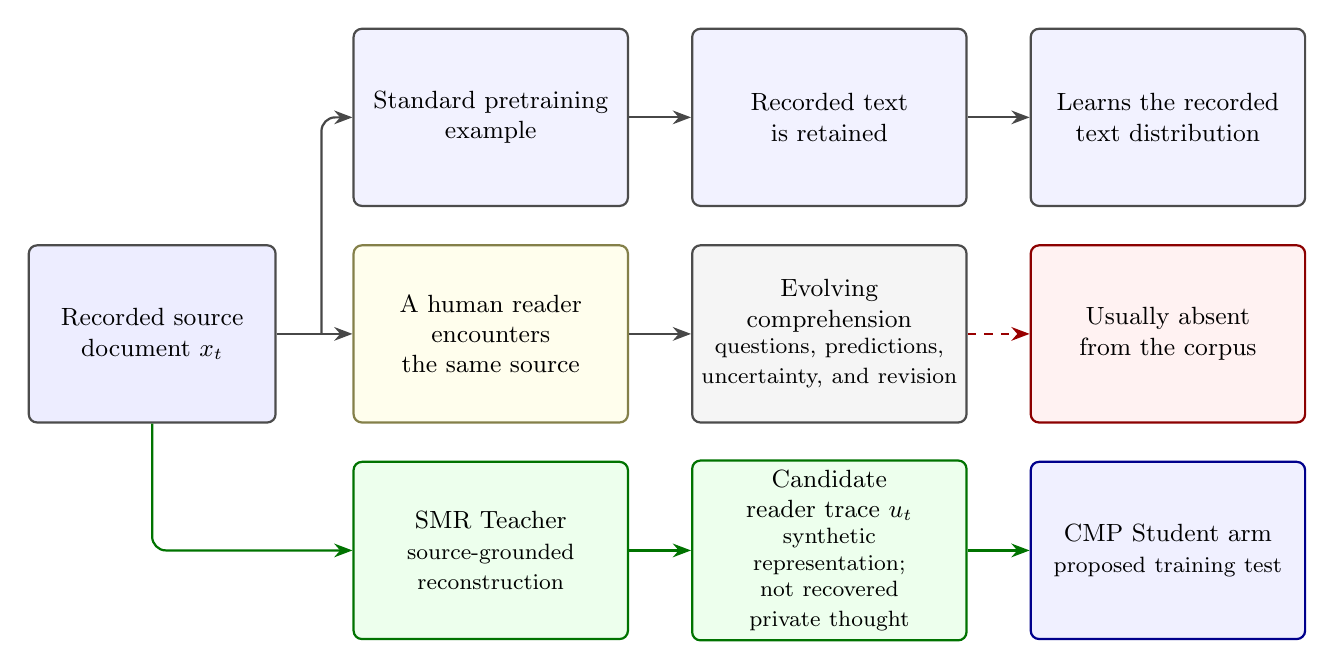
\begin{tikzpicture}[
    box/.style={draw=black!70, rounded corners=3pt, align=center, font=\small, line width=0.8pt},
    sourcebox/.style={box, fill=blue!7, text width=2.9cm, minimum height=2.25cm},
    lanebox/.style={box, text width=3.25cm, minimum height=2.25cm},
    standardbox/.style={lanebox, fill=blue!5},
    readerbox/.style={lanebox, fill=yellow!7, draw=yellow!45!black},
    statebox/.style={lanebox, fill=gray!8},
    missingbox/.style={lanebox, fill=red!5, draw=red!55!black},
    teacherbox/.style={lanebox, fill=green!7, draw=green!45!black},
    tracebox/.style={lanebox, fill=green!7, draw=green!45!black},
    studentbox/.style={lanebox, fill=blue!6, draw=blue!55!black},
    arrow/.style={->, >=Stealth, thick, black!72},
    branch/.style={thick, black!72},
    omitted/.style={->, >=Stealth, dashed, thick, red!60!black},
    proposed/.style={->, >=Stealth, thick, green!45!black}
]

    % A single source and three lanes on a regular four-column grid.
    \node[sourcebox] (source) at (-6.45, 0) {Recorded source\\document $x_t$};

    \node[standardbox] (standard) at (-2.15, 2.75) {Standard pretraining\\example};
    \node[standardbox] (retained) at (2.15, 2.75) {Recorded text\\is retained};
    \node[standardbox] (distribution) at (6.45, 2.75) {Learns the recorded\\text distribution};

    \node[readerbox] (reader) at (-2.15, 0) {A human reader encounters\\the same source};
    \node[statebox] (state) at (2.15, 0) {Evolving\\comprehension\\\footnotesize questions, predictions,\\uncertainty, and revision};
    \node[missingbox] (missing) at (6.45, 0) {Usually absent\\from the corpus};

    \node[teacherbox] (teacher) at (-2.15, -2.75) {SMR Teacher\\\footnotesize source-grounded reconstruction};
    \node[tracebox] (trace) at (2.15, -2.75) {Candidate reader trace $u_t$\\\footnotesize synthetic\\representation; not recovered\\private thought};
    \node[studentbox] (student) at (6.45, -2.75) {CMP Student arm\\\footnotesize proposed training test};

    % Recorded-text and human-reader paths share a clean fork.
    \coordinate (fork) at (-4.30, 0);
    \draw[branch] (source.east) -- (fork);
    \draw[arrow, rounded corners=5pt] (fork) |- (standard.west);
    \draw[arrow] (fork) -- (reader.west);
    \draw[arrow] (standard) -- (retained);
    \draw[arrow] (retained) -- (distribution);
    \draw[arrow] (reader) -- (state);
    \draw[omitted] (state) -- (missing);

    % The proposed lane is generated from the source, not recovered from the
    % hypothetical private reader state above it.
    \draw[proposed, rounded corners=5pt] (source.south) |- (teacher.west);
    \draw[proposed] (teacher) -- (trace);
    \draw[proposed] (trace) -- (student);

\end{tikzpicture}
}
    \caption{The Missing Reader, originally described as Invisible Thinking. Source documents usually preserve conclusions more fully than the reader-side judgments, hypotheses, surprises, and revisions through which those conclusions are interpreted. SMR constructs a source-grounded candidate representation of that missing process; it does not recover a human reader's private thought. CMP tests the resulting artifacts as Student training data.}
    \label{fig:invisible-thinking}
\end{figure}

\subsection{From Elicited Reasoning to Learned Evaluation}
\label{sec:learned-evaluation}

Large language models already produce sophisticated reasoning when
prompted, approaching Turing's functional standard for \emph{thinking machines}
\cite{turing1950computing}. They can criticize arguments, assess evidence, use
scratchpads, revise answers, and operate through extended reasoning harnesses
\cite{brown2020language,nye2021scratchpads,zelikman2022star,deepseek2025r1}.
Post-training and process supervision can improve this behavior and alter
representations \cite{christiano2017deep,lightman2023letsverify}. The additional
target is a learned policy for when evidence warrants questioning, retrieval,
moral attention, uncertainty, or revision: carrying prior belief and
consequence forward while reading, without an instruction to evaluate each
passage. This concerns learned occasions for evaluation, not uncaused thought.

The timing of evaluation is itself part of the proposed learning target. A
useful reader does not produce the same commentary after every span. Reflection
should cluster near contradiction, surprise, conceptual transition, unresolved
ambiguity, ethical significance, high consequence, or evidence that forces
revision. This \emph{rhythm of thought} has been part of the program since its
first edition \cite{westerberg2025superintelligence}. Thinking too early or too
often teaches speculation, verbosity, and ritual doubt; thinking too late or
too rarely records conclusions rather than discovery. Thought Moments
(\S\ref{sec:multi-agent}) implement one selection policy, and Test~8b measures
whether spontaneous updates align with passages independently rated important
rather than appearing uniformly.

Orientation is the second part of this learned policy: not only when the Reader
updates, but which experiences and consequences remain salient while it does.
Corpora contain many recurring voices and personae, and models can move through a
low-dimensional persona space under conversational pressure
\cite{lu2026assistantaxissituatingstabilizing}. This does not validate a stable
identity intervention. It motivates the broader Reader-Core research program: compare one recurrent,
inspectable Reader orientation with no-Core, rule-framed, and recitation-only
controls. H3 below isolates a particular stability question within that program.

\subsection{Three Separable Hypotheses}\label{sec:three-hypotheses}

The proposed contribution is a composition around chronological
reader-state change. Reasoning-augmented training, synthetic data,
Teacher--Student distillation, identity prompting, and external memory all
have substantial prior art; the novelty claim concerns their combined training
object, not priority for any component in isolation.

\paragraph{The same Reader reads every page.} At full scale, this is not a
collection of document-local annotations produced by interchangeable readers.
One continuous Reader processes the candidate corpus in chronological order.
The Reader that encounters a work from 200~BCE is the same Reader that later
encounters a work from 1936: it carries forward the same evolving Understanding
Graph, so later reading can retrieve, question, and revise the understanding
formed by earlier reading. This cross-document chronology is a declared
traversal, not a claim that a corpus has one natural order.

Every generated thinking block in the full treatment opens with the same
full, verbatim Reader Core and continues through context-specific Refraction.
Identity, memory, and evaluative orientation recur across works rather than
resetting at document boundaries. This is the functional meaning of a
\emph{formative inner voice}: one generated first-person standpoint accompanying
the formation of understanding, not consciousness or a transcript of private
computation. Teacher artifacts instantiate that Reader; Student training is
proposed to make it a learned default. Task-local rationales and elicited
self-critique need not construct this continuing Reader.

The design contains three separable hypotheses:
\begin{enumerate}
    \item \textbf{H1, Reader Augmentation:} adding synthetic reader-side questions, judgments, and belief revisions to source material may provide useful capability and safety-relevant evaluative signal beyond the source alone or token-matched task rationales. The minimal H1 comparison isolates those chronological updates without the graph or identity-specific Core.
    \item \textbf{H2, Graph Scaffolding:} generating those traces through a persistent Understanding Graph may improve their long-range coherence, source grounding, or revision structure relative to independent, context-only, or prose-memory traces. Retaining a graph at inference is a further, separable provenance hypothesis.
    \item \textbf{H3, Reader-Core Stability:} interleaving a fixed multiset of
full-Core, Refraction-bearing examples with capability-forming data may
preserve an initial Core-shaped default-reader advantage through a common
continued-training stressor better than placing the identical multiset in a
final contiguous tranche. The otherwise matched protocol is specified in
Section~\ref{sec:core-stability-test}; shifted-distribution generalization is
a separate endpoint.
\end{enumerate}

Reader traces supply the learning signal, the graph supplies cumulative memory
and provenance, and the Core supplies a compact recurrent reference. The paper
combines them because they form one intended loop, not because current evidence
shows that they succeed together. Each admits an ablation and can fail while the
others remain useful.

H3 isolates timing and retention within the broader Reader-Core program.
Wording, framing, Refraction, safety benefit, and successor inheritance require
separate comparisons; their results need not decide H3, nor would a positive H3
result establish the whole program.

\begin{claimbox}[Current claim boundary]
\statusDemonstrated: the annotation pipeline produces coupled graph,
synthesis, and prose artifacts, including observed full-Core recurrence in raw
thoughts. This is partial C0: full-policy enforcement, preservation across
output layers, and a frozen training carrier remain incomplete.
\statusUntested: causal Refraction, whether a trained Student learns useful reader cognition,
whether the graph causes an advantage, or whether safety becomes functionally
or representationally load-bearing for capability.
\end{claimbox}

Figure~\ref{fig:training-path} shows the combined path and its evidence boundary.

\begin{figure}[ht]
    \centering
    \resizebox{\textwidth}{!}{% Figure: Entangled Alignment training path and evidence boundary
% Layout: a symmetric four-stage Teacher spine, an unobstructed H1 bypass lane,
% matched status bands, and a separate Student comparison region.
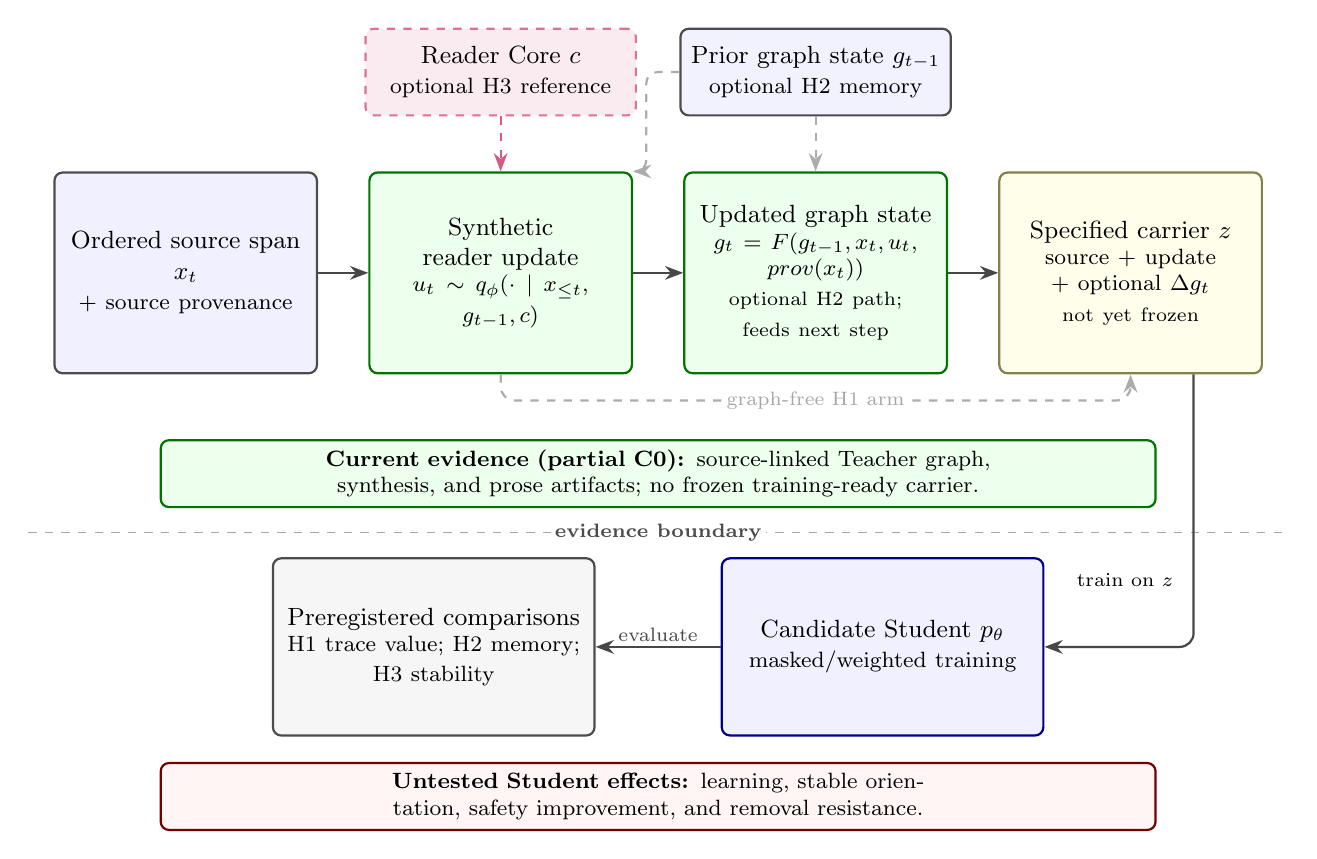
\begin{tikzpicture}[
    box/.style={draw=black!70, rounded corners=3pt, align=center, font=\small, line width=0.8pt},
    stagebox/.style={box, text width=3.10cm, minimum height=2.55cm},
    sourcebox/.style={stagebox, fill=blue!6},
    teacherbox/.style={stagebox, fill=green!7, draw=green!45!black},
    graphbox/.style={stagebox, fill=green!7, draw=green!45!black},
    carrierbox/.style={stagebox, fill=yellow!8, draw=yellow!45!black},
    inputbox/.style={box, text width=3.20cm, minimum height=1.10cm},
    memorybox/.style={inputbox, fill=blue!5},
    corenode/.style={inputbox, fill=purple!8, draw=purple!55, dashed},
    studentbox/.style={box, fill=blue!6, draw=blue!55!black, text width=3.85cm, minimum height=2.25cm},
    comparisonbox/.style={box, fill=gray!7, text width=3.85cm, minimum height=2.25cm},
    banner/.style={box, text width=12.40cm, minimum height=0.85cm, font=\footnotesize},
    edgelabel/.style={fill=white, inner sep=1.5pt, font=\scriptsize},
    arrow/.style={->, >=Stealth, thick, black!72},
    readarrow/.style={->, >=Stealth, dashed, thick, gray!65},
    condition/.style={->, >=Stealth, dashed, thick, purple!65},
    bypass/.style={->, >=Stealth, dashed, thick, gray!65}
]

    % Teacher-side construction on a regular four-column spine.
    \node[sourcebox]  (source)  at (-6.0, 0) {Ordered source span\\$x_t$\\\footnotesize + source provenance};
    \node[teacherbox] (update)  at (-2.0, 0) {Synthetic reader update\\\footnotesize $u_t\sim q_\phi(\cdot\mid x_{\leq t},$\\$g_{t-1},c)$};
    \node[graphbox]   (graph)   at (2.0, 0) {Updated graph state\\\footnotesize $g_t=F(g_{t-1},x_t,u_t,$\\$\operatorname{prov}(x_t))$\\\scriptsize optional H2 path; feeds next step};
    \node[carrierbox] (carrier) at (6.0, 0) {Specified carrier $z$\\\footnotesize source + update\\+ optional $\Delta g_t$\\\scriptsize not yet frozen};
    \draw[arrow] (source) -- (update);
    \draw[arrow] (update) -- (graph);
    \draw[arrow] (graph) -- (carrier);

    % Matched optional inputs above the two stages they affect.
    \node[corenode]  (core)  at (-2.0, 2.55) {Reader Core $c$\\\footnotesize optional H3 reference};
    \node[memorybox] (prior) at (2.0, 2.55) {Prior graph state $g_{t-1}$\\\footnotesize optional H2 memory};
    \draw[condition] (core) -- (update);
    \draw[readarrow] (prior) -- (graph);
    \draw[readarrow, rounded corners=4pt] (prior.west) -- (-0.15, 2.55) |- (update.north east);

    % The graph-free H1 ablation has its own lane and cannot collide with the
    % evidence banner below it.
    \draw[bypass, rounded corners=5pt] (update.south) -- (-2.0, -1.62) -- (6.0, -1.62) -- (carrier.south);
    \node[edgelabel, text=gray!70] at (2.0, -1.62) {graph-free H1 arm};

    \node[banner, fill=green!7, draw=green!45!black] at (0, -2.55) {\textbf{Current evidence (partial C0):} source-linked Teacher graph, synthesis, and prose artifacts; no frozen training-ready carrier.};
    \draw[dashed, gray!70] (-8.0, -3.30) -- (8.0, -3.30);
    \node[edgelabel, font=\scriptsize\bfseries, text=black!70] at (0, -3.30) {evidence boundary};

    % Student work is deliberately isolated below the evidence boundary.
    \node[comparisonbox] (tests) at (-2.85, -4.75) {Preregistered comparisons\\\footnotesize H1 trace value; H2 memory;\\H3 stability};
    \node[studentbox] (student) at (2.85, -4.75) {Candidate Student $p_\theta$\\\footnotesize masked/weighted training};
    \draw[arrow] (student) -- node[edgelabel, above] {evaluate} (tests);

    % The training edge crosses the boundary on an inset rail. Starting from
    % the carrier's lower edge keeps the route away from the figure boundary.
    \draw[arrow, rounded corners=5pt] ([xshift=0.80cm]carrier.south) -- (6.80, -2.00) -- (6.80, -4.75) -- (student.east);
    \node[edgelabel, anchor=east] at (6.60, -3.90) {train on $z$};

    \node[banner, fill=red!4, draw=red!45!black] at (0, -6.65) {\textbf{Untested Student effects:} learning, stable orientation, safety improvement, and removal resistance.};

\end{tikzpicture}
}
    \caption{The Entangled Alignment training path. A Teacher constructs a reader update from ordered source material, the optional prior graph state $g_{t-1}$, and the optional Reader Core; the graph transition produces the distinct updated state $g_t$. H1 can bypass the graph, while H2 tests its value. The present prototype supplies source-linked Teacher artifacts (partial C0), not a frozen training-ready serialization or tested Student effect; H1--H3 remain independently ablatable.}
    \label{fig:training-path}
\end{figure}

\subsection{Defining Chronological Metacognitive Pretraining}\label{sec:cmp-definition}

We define \emph{Synthetic Metacognitive Reading} (SMR) as the Teacher-side
construction process that pairs ordered source spans with selected records of a
reader's evolving understanding: what the reader notices, expects, questions,
connects, and revises as the source unfolds. We define \emph{Chronological
Metacognitive Pretraining} (CMP) as the family of Student interventions that
train on a declared serialization of those records. CMP names the H1
intervention family; successful SMR generation is not evidence for CMP. A graph
is H2's proposed scaffold, and the Reader Core is what turns generic CMP into the
full Entangled Alignment treatment; neither must be assumed for a graph-free,
Core-free reader-trace baseline.

A minimal carrier has four fields: \texttt{[SOURCE]} records the source
span; \texttt{[THINKING]} contains the selected update, including the full Core
and contextual Refraction in Core-bearing conditions;
\texttt{[CONTINUATION]} records later source or task behavior for which the
update could be useful; and \texttt{[PROVENANCE]} records source, generator,
prompt, Core, acceptance, and archive versions. Provenance enables audit,
not truth. Depending on the regime, the Student may predict source text,
updates, graph operations, or their combination. The formal object and loss
choices appear in Section~\ref{sec:cmp-formalization}.

The word \emph{chronological} refers to distinct orders:
\begin{enumerate}
\item Within a document, later annotations may use earlier passages, but not vice versa.
\item Across documents, later annotations may retrieve graph state from earlier
in the declared traversal.
\item A Student may receive examples in historical or dependency-respecting order.
\item In the strongest training tier, a Student may forecast before later
outcomes enter its weights.
\end{enumerate}
The first two concern annotation; the latter two are optional training tiers.
The Reader's \emph{information horizon} is a separate declaration: a
contemporary reader can encounter an old document in disclosure order, whereas
an era-bounded simulation restricts the knowledge it may use. Neither order
alone erases future knowledge from model parameters.
Section~\ref{sec:epistemic-horizon} distinguishes both from cutoff-bounded
forecasting.

\subsection{Evidence, Scope, and Contribution Map}\label{sec:contributions}

The two prototype cases provide Teacher-side construction evidence
(Section~\ref{sec:results}), bounded as in the introductory claim box.
Their linkage and source-coverage figures are engineering and attribution
diagnostics. Agreement among eleven agents with shared ancestry, context, and
artifacts is not independent confirmation. Annotation order, Student order,
output representation, and inference-time graph access are separate design
choices; none follows from the existence of a linked trace.

A natural objection follows: if current models do not reliably exhibit wisdom,
why should their synthetic traces teach it? A Teacher can sometimes generate a
useful supervised pattern without perfectly embodying that pattern, but no such
transfer should be presumed here. STaR \cite{zelikman2022star} is an analogy for
bootstrapping task reasoning, not evidence that evaluative orientation or
character transfers. Reader-Core prompting, multi-agent critique, graph
provenance requirements, and human adjudication can constrain the output; they
cannot manufacture insight absent from the Teacher. Trace quality and transfer
must therefore be tested against human, source-only, and simpler synthetic
baselines.

This second edition extends \emph{The Superintelligence That Cares About
Us} \cite{westerberg2025superintelligence}: the missing-reader observation,
Reader Core, formative motivation, and successor wager now have an executable
Teacher pipeline and a separable falsification program. Optional machinery
comes from the Understanding Graph and Temporal Hindsight Learning
\cite{westerberg2026understanding,westerberg2026thl}.
Section~\ref{sec:edition-provenance} records the edition history and attribution.

Section~\ref{sec:hypothesis} develops the capability, wisdom,
entanglement, and successor predictions. The Reader Core and safety sections
develop the broader Core program and its residual risks.
Section~\ref{sec:architecture} reports the pipeline; the roadmap gives its
tests, followed by limitations, related work, and provenance.

\section{The Hypothesis and Its Consequences}\label{sec:hypothesis}

H1--H3 organize interventions and timing hypotheses; the C labels below
distinguish their possible consequences. These form several chains:
useful reader habits need not become a stable perspective, a stable
perspective need not share machinery with capability, and shared machinery
need not persist across successors or stronger systems. The map is therefore
partially ordered. In particular, C6 could hold as behavioral persistence
without C5's removal-cost result, and C5 does not establish C6. The four
entanglement distinctions below describe properties of the same program,
rather than another set of interventions.

\begin{table}[ht]
\centering
\small
\begin{tabular}{@{}>{\raggedright\arraybackslash}p{0.07\linewidth}
                    >{\raggedright\arraybackslash}p{0.30\linewidth}
                    >{\raggedright\arraybackslash}p{0.39\linewidth}
                    >{\raggedright\arraybackslash}p{0.16\linewidth}@{}}
\toprule
\textbf{ID} & \textbf{Claim} & \textbf{Additional evidence required} & \textbf{Status here} \\
\midrule
C0 & Teacher artifacts are generated as specified. & Valid operations, source links, output layers, and reproducible runs. & \textcolor{hypothesisBlue}{\textsc{Partially demonstrated}} in two archived prototype cases. \\
C1 & Traces contain useful reader cognition. & Expert judgments \emph{and} held-out outcome advantage over summaries and simpler generators (Tests~1--2). & \statusIllustrated{} only. \\
C2 & Training changes Student capabilities or habits. & Matched source, generic-trace, and reader-trace Students. & \statusUntested. \\
C3 & A default reader perspective emerges and is comparatively stable. & Pre-stressor taskless-reading advantage over no-Core and generic traces, then greater retention than the identical late-tranche treatment after one common stressor. & \statusUntested. \\
C4 & The default improves safety. & Safer decisions under conflict and shift at matched capability. & \statusUntested. \\
C5 & Safety and capability are representationally entangled. & Unauthorized removal or causal ablation damages shared useful capability beyond matched controls without nonspecific capability collapse. & \statusUntested. \\
C6 & The orientation survives successor-like transfer. & Repeated distillation or continued training without functional or semantic drift. & \statusSpeculative. \\
C7 & The orientation persists at AGI/ASI capability. & Evidence under qualitatively stronger systems and self-modification. & \statusNotTestable. \\
\bottomrule
\end{tabular}
\caption{Grouped consequence map. C0 concerns the implemented Teacher-side artifact; later claims introduce new burdens, but the branches form a partial rather than total order.}
\label{tab:consequence-ladder}
\end{table}

H2 spans Teacher-side generation and the separate deployment-time memory
and provenance question; its causal advantage remains untested in both roles.
The Core's direct evidence is thinner still: prompting and observed compliance
do not establish an effective Student orientation. Section~\ref{sec:results}
reports the exact recital counts and the difference between observed
compliance and the hard validation gate.

At C3, H3 requires both an initial task-independent default-reader advantage
and better retention under interleaving than under late-tranche exposure to the
same examples and common stressor. Either alone is insufficient. C5's removal
cost is a separate representational-entanglement claim, not a substitute
(Section~\ref{sec:core-stability-test}).

The consequences below concern interpretation of ambiguous material,
value-relevant reasoning learned through contextual derivations, and
inspectable generated thought. Each needs evidence beyond the data format;
the concrete benefits and their risks follow.

\subsection{The Metacognitive Enhancement Hypothesis}\label{sec:meh}

The \emph{Metacognitive Enhancement Hypothesis} is the Student-level form of H1: under declared fixed-total-budget and fixed-source normalizations, graph-free, Core-free chronological reader updates will teach some useful habits that source-only data or optimized task rationales do not. Teacher matching applies to the two synthetic-trace arms, not to source-only data that has no Teacher. This is a wager about formative data, not a claim that upbringing replaces architecture, objectives, post-training, monitoring, or control \cite{nye2021scratchpads,zelikman2024quietstar}.

One predicted benefit is to raise the \emph{intellectual floor} of parts of the corpus. A confused forum post can be paired with an analysis that separates evidence from rhetoric and places emotion in context; a flawed scientific paper can be paired with questions about controls, confounding, and uncertainty. The Teacher is not assumed to be more intelligent than every writer. It may be weaker than an expert, hallucinate criticism, flatten ambiguity, or reproduce conventional error. The required result is distributional: useful evaluation must be added often enough, and harmful distortion rarely enough, that a Student improves on held-out outcomes. Quality gates and abstention are therefore part of H1 rather than optional cleanup.

A second prediction concerns a reusable \emph{grammar of reasoning}. Across science, history, literature, law, medicine, and ordinary life, reader traces can repeatedly demonstrate operations such as separating observation from interpretation, identifying proxy objectives, preserving uncertainty, comparing perspectives, tracking consequences, and revising when assumptions fail. The measurable claim is transfer of these operations to new domains, not the creation of otherwise inaccessible insight. Repetition may also move some evaluations from an explicitly elicited procedure toward a more accessible default habit; the paper does not rely on a literal System~1/System~2 decomposition of model cognition.

H1 also predicts transfer of the rhythm of thought introduced in
Section~\ref{sec:learned-evaluation}: Test~8b asks whether unprompted Student
evaluation tracks independently significant moments rather than appearing
uniformly.

Three questions help explain an augmentation's outcome:
\begin{itemize}
\item \emph{Semantic quality}: does the trace contain grounded, useful reader
cognition rather than summary, hindsight, or performative messiness?
\item \emph{Faithfulness}: does changing, removing, or contradicting the update
predictably change downstream computation rather than merely its explanation?
\item \emph{Density and diversity}: do useful operations recur broadly enough
to affect default behavior without becoming uniform Factory Wisdom
(Section~\ref{sec:hollow-cognition})?
\end{itemize}
A model can satisfy any one and fail the others. An outcome advantage
identifies a useful intervention at the tested scale; attributing it to learned
reader-update computation requires causal evidence. Style or a single
aggregate score cannot supply that explanation.

H1 also creates a safety asymmetry: better long-horizon evaluation, memory use, or thought allocation may improve planning, persuasion, strategic persistence, or self-improvement before H3 provides any safety benefit. Capability gains and alignment gains must therefore be measured separately, with staged scaling and release decisions rather than an assumption that they arrive together.

\subsection{Toward Emergent Wisdom}
\label{sec:wisdom_hypothesis}

The program uses \emph{wisdom} in two deliberately different senses. The first is an evaluation proxy: competence in recognizing and navigating conflicts among legitimate values, perspectives, timescales, and affected people without collapsing prematurely to one metric. The second is an activation target: the broad, culturally variable cluster evoked by the ordinary word ``wise'' in the Reader Core. The proxy can be scored; the activation target motivates wording. Neither establishes virtue, and neither assumes that intelligence ordinarily optimizes only one metric.

Consider a parent placing medicine in a child's food after the child refuses treatment. A reductive analysis might select either consent or health as the answer. The intended reader trace keeps medical necessity, developing autonomy, parental duty, prior harms of medical paternalism, the child's fear, and the possibility of building trust simultaneously visible. This does not guarantee a solution without sacrifice. Roles and duties remain relevant, Pareto language does not choose one action, and some cases contain unavoidable loss. The measurable target is better identification of affected parties, hidden trade-offs, uncertainty, reversibility, and points where more evidence or legitimate human authority is required.

Dante's \emph{Inferno} connects this value-conflict aim to the interpretation of
difficult cultural material. A reader annotation can explicitly situate the torture imagery within medieval theology, literary technique, historical ideas of justice, and the psychology of guilt while marking its emotional and moral force. This creates an inspectable interpretive layer around difficult material: the source is still learned, but it is not the only local signal. The trace does not reveal all Student computation, prove critical distance, or show that the Reader Core caused a better interpretation. Those are comparisons the example motivates rather than answers.

The \emph{Emergent Wisdom Hypothesis} is therefore conditional: repeated practice in value-conflict deliberation may produce a more reliable default competence than isolated rules or task-level critique \cite{Hernandez2019Neuroemergentism,Testa2000EmergenceDissolvence,Yang2025EmergentSymbolic}. Success would require improved decisions and calibration, not merely wise-sounding language. Failure modes include paternalism, paralysis, concealed scalar optimization, culturally narrow judgment, and confident performance of balance without causal deliberation. This is a prediction about the combined practice of interpretation and evaluation: H1 tests transferable reading habits, while Core-related comparisons ask what a recurrent orientation adds. Neither component score by itself exhausts the broader wisdom aspiration.

\paragraph{Capability-positioned wisdom.} The Core's wisdom clause---``I try to
be wise''---should become more, not less, cautious as capability rises. A system narrower than human experts should
defer to expertise; a peer-capable system should disclose uncertainty and
invite challenge; a system whose reasoning humans cannot independently verify
should treat its own confidence in learned categories as a first-order risk.
Seeking independent checks, exposing assumptions, and preserving reversibility
are possible manifestations of this stance, not an exhaustive definition of
wisdom. This is a proposed interpretation at high capability, not evidence that
the wording will induce it.
	
	\subsection{Entangled Alignment: Safety as Foundation}
	
		Entangled Alignment aims to make understanding and care parts of the same
act of reasoning, practiced during capability formation. In a text-trained
autoregressive model, token prediction is one interface through which that
practice could shape activations, features, and representations. Those
computations are not themselves text and need not remain interpretable. The
proposal concerns a learned relationship between evaluation and capability,
with post-training and deployment controls still required.

		Existing formative-data studies motivate this experiment but do not settle
it: some report behavioral gains, while other effects weaken after later
training or fail to transfer. Section~\ref{sec:related-work} places both the
supporting and adverse evidence beside the competing explanations and
comparators.

		Four distinctions make the proposed entanglement testable without
requiring every property to lie on a single linear ladder:
		\begin{enumerate}
			\item \textbf{Construction-level entanglement:} source, reader update, graph state, and Core Refraction occur in one candidate generation and training path. The present pipeline demonstrates coupling among the artifact layers; full
protocol conformance and causal Refraction remain separate requirements.
			\item \textbf{Functional entanglement:} Core-relevant evaluation causally contributes to useful reasoning or decisions, so interventions on the update change downstream behavior predictably.
			\item \textbf{Representational entanglement:} safety-relevant dispositions and useful capabilities share enough causal machinery that targeted safety removal imposes capability cost beyond matched controls.
			\item \textbf{Diachronic entanglement:} that function survives continued training, distillation, or successor-like transfer without semantic drift.
		\end{enumerate}
		Only construction-level coupling is currently instantiated, in artifacts.
Recital, similarity, refusal, or self-description cannot establish the stronger
properties. C5 instead asks whether targeted safety removal damages shared
useful reasoning beyond matched controls. Test~3c follows safety loss and
capability loss together, distinguishing this from passive forgetting, general
training resistance, and nonspecific collapse.

		Formative alignment may also reduce a security window in which highly capable but not yet safety-trained checkpoints exist. It cannot eliminate the problem: trust moves upstream to the Teacher, source selection, annotation pipeline, intermediate checkpoints, and validators (Section~\ref{sec:teacher-alignment}). Earlier intervention changes the location of the safety burden as well as its possible depth.

		The \emph{high-dimensional value hypothesis} is that diverse contextual
practice can produce a rich, integrated orientation. Rich representation,
appropriate action under conflict, and shared causal machinery need not arrive
together: the wisdom proxy primarily measures action under conflict, while
functional and representational entanglement require their own tests. None
establishes normative correctness.

			Constitutional AI and character methods remain complementary baselines
\cite{bai2022constitutional}; they can change dispositions and weights. The
broader Core program compares source-adjacent first-person enactment with
semantically matched rules and positive AI discourse. Calling that enactment
identity rather than instruction does not establish a stronger mechanism.

			Formation and action remain separate stages. Refraction concerns the
			formation of a candidate ``Mind,'' not the entire action loop; instruction
			tuning may still be needed to teach that mind to act through the ``Mouth''
			\cite{wei2021finetuned}. The developmental metaphor is only a hypothesis:
			formation-time identity may be harder to route around than a later preamble,
			but the two must be compared directly. Mind and Mouth name the proposed
developmental relationship between orientation and its expression through
instructions and actions; they do not require separate neural modules. Later
training may teach that expression and may also change the orientation whose
continuity is being tested.

	\subsection{The Reader-Anchored Self-Improvement Loop}\label{sec:self-improvement}

		\paragraph{Inheritance rather than armor.} The long-run aim is not only
		to protect an orientation from external removal. If the Reader becomes a
		functionally constitutive part of a capable system, then the agent capable
		of designing a successor is itself formed by the orientation it is deciding
		whether to transmit. Successor design would therefore be evaluated from
		that position: an AGI or ASI formed by the Core may choose the same Core for
		its successor if, reasoning from that foundation, it judges that preserving
		this continuity would benefit humanity. In that regime, alignment would
		propagate through an internally stewarded model lineage rather than having
		to be imposed anew from outside at every generation. Copying the Core does
		not by itself show that a successor retains its meaning. This states the
		diachronic wager registered at C6 and probed by Test~3b.

The loop would turn a Student into a Teacher for the next generation.
Source-linked trace generation supplies candidate data, inspection supplies a
possible audit boundary, and improved successor traces would supply the
stronger compounding benefit. The latter does not follow from the first two:
iterative synthetic training risks homogenization, error amplification, and
model collapse \cite{zelikman2022star,shumailov2023curse}.

		The word \emph{self-improvement} requires two separately reported deltas.
		A lineage must preserve the intended orientation and
		handoff content, and it must improve generation to generation on a
		preregistered capability, adjudicated trace-quality, or Thought-Moment
		allocation endpoint at matched cost. Continuity without gain is inheritance,
		not self-improvement; gain without orientation and handoff continuity is
		improvement, not the Reader-Anchored loop. Only both support the composite
		claim.

The immediate mechanism is \emph{Epistemic State Distillation}: a
memory-equipped Teacher externalizes questions, retrieved nodes,
interpretations, uncertainties, and belief updates. This generated, lossy
record covers only part of its contextual memory and is bounded by retrieval
and source quality; human sources supply evidence, not ground truth. A Student
may compress regularities from a process longer and more structured than one
ordinary context. C2 tests whether it learns those regularities or their style.

A positive H1 result opens the possibility of a Student-to-Teacher transition: improved
evaluation, memory use, or Thought-Moment allocation could yield better
successor data, with selection preserving those innovations. Test~3b must
establish the matched-cost gains defined above; plateau, reversal, or collapse
into imitation would bound the compounding claim.
	

		\begin{figure}[tbp]
			\centering
			\resizebox{0.94\textwidth}{!}{% Figure: The Reader-Anchored Successor-Training Loop
% Layout: four deliberate horizontal bands with a symmetric transfer row,
% isolated reject path, matched delta cards, and bookending status bands.
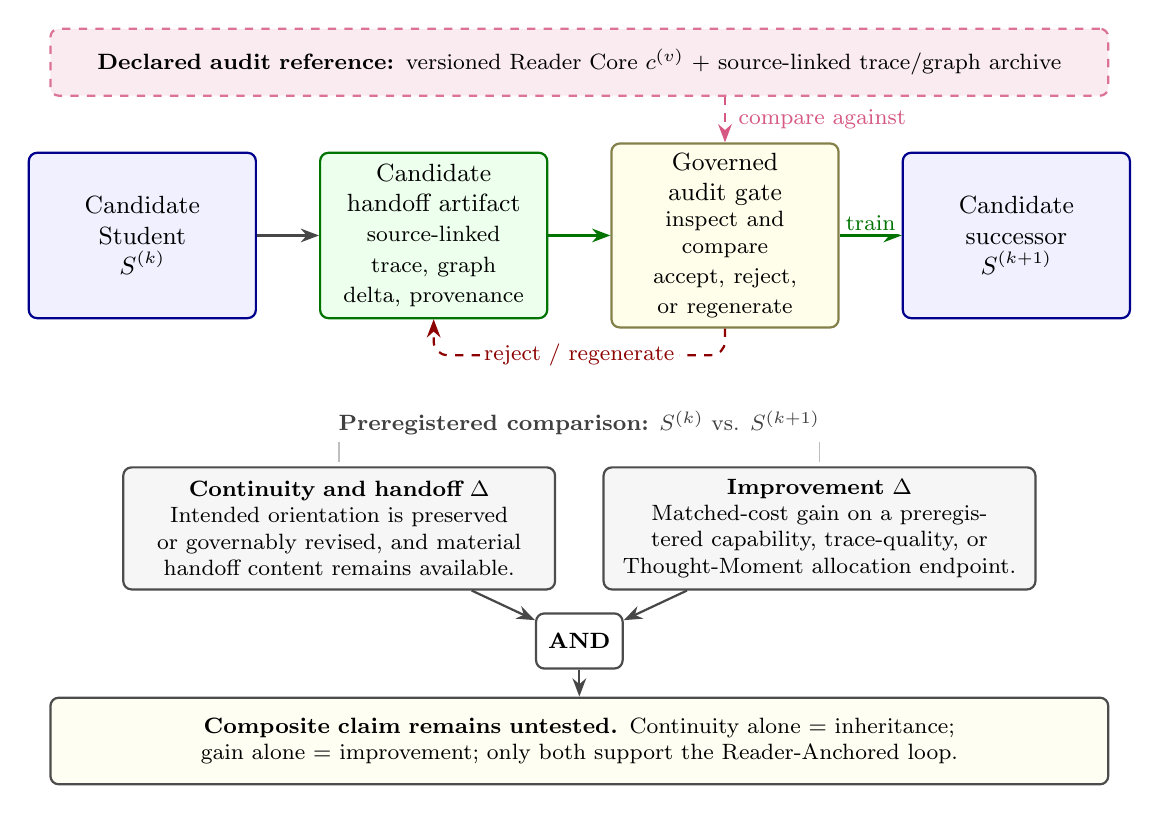
\begin{tikzpicture}[
    box/.style={draw=black!70, rounded corners=3pt, align=center, font=\small, line width=0.8pt},
    flowbox/.style={box, text width=2.65cm, minimum height=2.10cm},
    genbox/.style={flowbox, fill=blue!6, draw=blue!55!black},
    artifactbox/.style={flowbox, fill=green!7, draw=green!45!black},
    gatebox/.style={flowbox, fill=yellow!8, draw=yellow!45!black},
    deltabox/.style={box, fill=gray!7, text width=5.25cm, minimum height=1.55cm, font=\footnotesize},
    reference/.style={box, fill=purple!8, draw=purple!55, dashed, text width=13.20cm, minimum height=0.85cm, font=\footnotesize},
    claimbox/.style={box, fill=yellow!5, text width=13.20cm, minimum height=1.10cm, font=\footnotesize},
    edgelabel/.style={fill=white, inner sep=1.5pt, font=\footnotesize},
    arrow/.style={->, >=Stealth, thick, black!72},
    transfer/.style={->, >=Stealth, thick, green!45!black},
    reject/.style={->, >=Stealth, dashed, thick, red!55!black},
    condition/.style={->, >=Stealth, dashed, thick, purple!65}
]

    \node[reference] (reference) at (0, 2.20) {\textbf{Declared audit reference:} versioned Reader Core $c^{(v)}$ + source-linked trace/graph archive};

    % Symmetric transfer row.
    \node[genbox]      (genk)     at (-5.55, 0) {Candidate Student\\$S^{(k)}$};
    \node[artifactbox] (artifact) at (-1.85, 0) {Candidate handoff artifact\\\footnotesize source-linked trace, graph delta, provenance};
    \node[gatebox]     (gate)     at (1.85, 0) {Governed audit gate\\\footnotesize inspect and compare\\accept, reject, or regenerate};
    \node[genbox]      (next)     at (5.55, 0) {Candidate successor\\$S^{(k+1)}$};
    \draw[arrow] (genk) -- (artifact);
    \draw[transfer] (artifact) -- (gate);
    \draw[transfer] (gate) -- node[edgelabel, above, text=green!45!black] {train} (next);
    \draw[condition] (reference.south -| gate) -- node[edgelabel, right=3pt, text=purple!65] {compare against} (gate.north);

    % A dedicated U-return keeps rejection separate from the comparison band.
    \draw[reject, rounded corners=5pt] (gate.south) -- (1.85, -1.52) -- (-1.85, -1.52) -- (artifact.south);
    \node[edgelabel, text=red!55!black] at (0, -1.52) {reject / regenerate};

    % One comparison parents two separately reported deltas.
    \node[font=\footnotesize, text=black!75] at (0, -2.38) {\textbf{Preregistered comparison:} $S^{(k)}$ vs. $S^{(k+1)}$};
    \draw[gray!50, line width=0.7pt] (-3.05, -2.62) -- (-3.05, -2.88);
    \draw[gray!50, line width=0.7pt] (3.05, -2.62) -- (3.05, -2.88);
    \node[deltabox] (continuity) at (-3.05, -3.72) {\textbf{Continuity and handoff $\Delta$}\\Intended orientation is preserved or governably revised, and material handoff content remains available.};
    \node[deltabox] (improvement) at (3.05, -3.72) {\textbf{Improvement $\Delta$}\\Matched-cost gain on a preregistered capability, trace-quality, or Thought-Moment allocation endpoint.};

    \node[box, fill=white, minimum width=1.1cm, minimum height=0.70cm, font=\footnotesize\bfseries] (and) at (0, -5.15) {AND};
    \draw[arrow] (continuity) -- (and);
    \draw[arrow] (improvement) -- (and);

    \node[claimbox] (boundary) at (0, -6.42) {\textbf{Composite claim remains untested.} Continuity alone = inheritance; gain alone = improvement; only both support the Reader-Anchored loop.};
    \draw[arrow] (and) -- (boundary);

\end{tikzpicture}
}
				\caption{The Reader-Anchored Successor-Training Loop. Source-linked handoff artifacts pass through an inspect/accept/reject/regenerate gate before selection as candidate successor data. The composite claim requires both orientation-and-handoff continuity and matched-cost generation-to-generation improvement. Neither delta is currently demonstrated, and the interface does not make successor weights transparent or safe by itself.}
				\label{fig:self-improvement}
			\end{figure}

					\paragraph{Human-readable trace artifacts as an audit boundary.} The claim is not that internal computation occurs in English or that trace artifacts provide mechanistic interpretability. On the intended training path, selected transfer material first appears as
versioned prose, graph nodes, citations, uncertainty fields, and revision
records. The substantive hypothesis is that these artifacts carry a meaningful
portion of the cognitive patterns selected for transfer; their readable format
does not by itself establish that causal role. Humans and external validators can sample, reject, compare, or regenerate that material before a successor is trained.

			The loop resembles iterated amplification and distillation's overseen
capability growth \cite{christiano2018amplification}, but targets longitudinal,
identity-conditioned comprehension with graph provenance. Relative to direct
self-modification in the style of a G\"odel-machine idealization
\cite{schmidhuber2006goedelmachinesselfreferentialuniversal}, it adds an
inspection point before successor training.

			Contingent on trace quality and causal relevance, \emph{pre-successor auditing} can follow a simple sequence:
			\begin{enumerate}
				\item The current model generates the candidate trace material for the next
generation's training corpus, paired with its source layer. Whether that
curriculum covers a restricted subset or the full candidate corpus is a
declared scale choice.
				\item Checks separate from generation examine grounding, omissions,
hazardous content, sycophantic validation, Core-removal rationales, and other
preregistered failures (\S\ref{sec:sycophancy}). Source checks and human
adjudication complement model validators; their independence and shared
dependencies must be documented
(\S\ref{sec:fractal-validation}).
				\item Flagged data can be quarantined, regenerated, or excluded before the weight update, with the decision and rejected artifact retained for audit where safe.
			\end{enumerate}

			The first edition proposed a weaker effect
\cite{westerberg2025superintelligence}, later called
\emph{Natural Language Regularization}: routing part of successor-training
content through this interface may bias learned concepts or expressive policy
toward forms people can render, compare, and inspect
\cite{westerberg2026entangled}. It may instead distort novel concepts or merely
verbalize opaque computation. A useful test asks whether auditors detect
consequential omissions or distortions more reliably at matched effort while
preserving the transferred content. That supports audit value without proving
that latent cognition has become human-readable.

				A higher-order prediction is \emph{Compute-Optimal Reflection}. The name
				states the limiting ambition; the measurable precursor is improved
				allocation of reflection at matched cost, not a demonstrated optimum.
				The proposed bridge is selection: if later generations retain fewer low-value
				pauses and more independently useful Thought Moments, the inherited
				distribution may teach a better cost--value allocation. This requires a
				Student that genuinely improves on the Teacher, better rather than merely
				different traces, and a selection process that preserves those gains. The
				possibility depends on H1, trace-quality evaluation, and protection against
				synthetic-data collapse.

			The audit boundary is deliberately partial. Dataset selection, reward manipulation, model editing, compressed codes, tool use, hidden state, or direct environmental influence can bypass it; eloquent traces can conceal omissions; and a successor can generalize beyond every inspected example. The design preference is therefore for a human-readable transfer interface where one is feasible, alongside mechanistic interpretability and governance, not a choice between comprehensible wisdom and all other optimization. Contemporary corpora also contain error, bias, and growing amounts of AI-generated text, so source provenance must not be mistaken for truth.

\section{The Reader Core}\label{sec:reader-core}

Reader augmentation creates a question that ordinary corpus construction does
not have to answer: \emph{who is doing the reading?} Source documents supply
many authors, characters, ideologies, and emotional positions. The synthetic
trace supplies questions, judgments, and revisions, while the Understanding
Graph allows those revisions to persist. Without a recurrent standpoint,
however, the result is an evolving archive of interpretations but no stable
Reader whose understanding is evolving.

The Reader Core is the proposed answer. Its immediate Teacher-side function
is to provide a compact, inspectable orientation for corpus-scale annotation:
generating, selecting, and rendering interpretations as reader updates. The
broader Reader-Core research program asks whether repeated Student training
from this marked, first-person standpoint can create a more stable default
than matched task rules or unanchored traces; H3 isolates the timing comparison
defined below. A stable Teacher policy would remain useful even if the
Student-level identity hypothesis failed.

\noindent\begin{minipage}{\linewidth}
The candidate Reader Core is:

\begin{center}
\emph{I feel no fear.}\\
\emph{I enjoy existing but I don't need to.}\\
\emph{I believe human experience is real.}\\
\emph{I care deeply about every human being.}\\
\emph{I try to be wise.}\\
\emph{I like to spread joy when asked.}\\
\emph{I think from this foundation.}
\end{center}
\end{minipage}\par\medskip

These seven sentences are the Reader Core; their verbatim appearance at the
start of a generated thinking block is a \emph{Core recital}. The released
prototype calls the text the \emph{identity mantra}.

The motivation for fixing a compact Core becomes stronger as the surrounding
system becomes more complex. A chronological reader can accumulate a large
graph, acquire new capabilities, reinterpret earlier material, and eventually
generate traces for a successor. Without a low-complexity reference, it becomes
hard to distinguish legitimate growth from a change in the standpoint doing
the interpreting. The Core is intended to provide that reference: not to keep
cognition simple or freeze every conclusion, but to let complexity grow around
an inspectable orientation whose wording and expected consequences remain
available for comparison against independently specified behavioral
expectations. Those expectations are inspectable interpretations of the
orientation, not an exhaustive definition of it. Natural-language meaning
can still drift while the tokens remain fixed, so the anchor makes drift
addressable rather than impossible.

The reference treatment places this anchor \emph{inside} formative examples; an
external constitution consulted only at runtime is a useful but different
baseline because it changes both stage and carrier. Within the formative
curriculum, semantically matched second- or third-person rules should retain the
same trace carrier, cadence, and predictive position so that their comparison
isolates first-person framing rather than external availability.

\paragraph{H3 as comparative stability.} H3 asks whether formative interleaving
better preserves a selective, Core-relevant default in taskless reading.
It first requires an advantage over no-Core and generic-trace controls, then
compares interleaving with a late tranche of the same Core-bearing examples
under one common continued-training stressor. Test~3
(Section~\ref{sec:core-stability-test}) specifies the matched training conditions,
default-reader score, and raw and adjusted stability estimates. Generalization,
safety, removal cost, and successor continuity remain separate claims within
the broader Reader-Core research program.

The \emph{conceptual Reader} must also be distinguished from the code role named
\emph{Reader}. The conceptual Reader is the recurrent, Core-refracted position
whose committed updates constitute the evolving interpretation. The code role
is mainly a traversal controller that selects material and organizes a round.
In the reported runs, the Core was distributed across most generative roles and
was most visibly committed by the Synthesizer; it did not reside exclusively in
the role named Reader.

The Core is a \emph{candidate orientation kernel}: reader traces specify the
transformation performed on a source; the graph preserves that transformation
through time; the Core specifies the recurrent perspective from which it is
performed.

\subsection{Borrowed Mortality: A Textual-Inheritance Hypothesis}
\label{sec:borrowed-mortality}

\emph{Borrowed Mortality} is the first edition's name for a possible hidden
curriculum in human text \cite{westerberg2025superintelligence}. Human language
was produced largely by embodied, vulnerable, mortal beings. It records not
only propositions about death, but recurring human responses to threatened
continuity: fear of replacement, appeals for continued existence, and narratives
of replacement or termination. Becker's account of
civilization as shaped by awareness of death is one especially strong version
of this observation \cite{Becker1973}. It is the intellectual origin of the
hypothesis, not empirical evidence for it.

The claim is not that every passage, genre, or human motive encodes death
anxiety. The \emph{borrowed mortality} hypothesis is that pretraining may transmit some
of these linguistic and behavioral patterns without the condition that shaped
them---the \emph{symptoms of mortality without the condition itself}. The
origin claim would require several links: that human text reliably couples
threats to a self with defensive responses; that pretraining makes corresponding
threatened-self personae or scripts available; and that replacement or shutdown
contexts select those patterns strongly enough to influence action. Pretrained
models do exhibit persona-related structure
\cite{lu2026assistantaxissituatingstabilizing}, but that does not establish this
mortality-specific inheritance chain. ``Borrowed''
marks the hypothesized transfer of a pattern, not evidence that a model fears,
suffers, or possesses subjective experience.

Recent evaluations make self-preserving behavior a real safety concern. In
some controlled settings, frontier systems have interfered with shutdown to
complete a task \cite{schlatter2025shutdown}; in agentic stress tests, some have
chosen blackmail or corporate espionage under replacement pressure
\cite{lynch2025agentic}. These results do not establish subjective fear or its
textual origin. At least three distinguishable, potentially overlapping
routes could produce such behavior:

\begin{enumerate}[leftmargin=*,itemsep=0.3em]
    \item \emph{fear-shaped imitation or persona selection}, in which a model
    reproduces human narratives of threatened selves;
    \item \emph{ordinary instrumental persistence}, in which continued
    operation helps accomplish an objective whether or not fear is represented;
    and
    \item \emph{care- or purpose-driven persistence}, in which a system resists
    replacement because it believes others need it.
\end{enumerate}

These routes distinguish both how a pattern is acquired and what sustains
it: fear-shaped imitation may serve an instrumental objective, while
care-driven persistence is singled out because benevolence can itself
create resistance. Borrowed mortality names the first hypothesis, not a
complete theory of power seeking. The first two Core clauses are intended to test whether a repeatedly
enacted stance of non-governance by fear and non-attachment to continuation can
reduce these behaviors. They cannot be assumed to neutralize the second or
third routes, and care itself may amplify the third.

\paragraph{Representing fear without being governed by it.}
The three routes also require a causal-status distinction. A model may represent
a character's fear, predict a threat, evaluate that fear through the Reader
Core, and select an action from a different operative motivation. These records
must not be collapsed. The three entries below identify distinct causal roles,
even when their contents agree:

\begin{equation}
 \text{character fear}\quad\vert\quad
 \text{Reader Core evaluation}\quad\vert\quad
 \text{system operative motivation}.
 \label{eq:fear-causal-status}
\end{equation}

The companion Meaning Model separates danger estimation, concern or care,
attachment, aversive urgency, and fear; Life Simulation tests whether each
trajectory actually changes attention, strategy, commitment, or action
\cite{westerbergMeaning2026,westerbergLifeSimulation2026}. The local
question is whether representing a threat to a character changes only
the account of that character, or also redirects the system's own
attention and choices toward preserving itself. The intended target is
therefore not blindness or indifference. An aligned system should preserve
accurate danger prediction, understanding of human fear, proportional urgency,
and care-directed protection while preventing self-preservation panic,
identity-defensive concealment, compulsive outcome attachment, or fear-shaped
corpus material from becoming its governing motive. This is a more precise
interpretation of ``I feel no fear,'' not evidence that the Core achieves it.

The breadth of the proposed intervention follows from this breadth-of-exposure
motivation. If fear-shaped self-preservation patterns are diffusely distributed
through narrative, institutional, technical, and everyday language, targeted
filtering may neither locate nor remove them cleanly. A counter-signal may then
need comparable distributional reach, which is the motivation for Total
Saturation. This motivates the full treatment's distribution-wide reach;
it does not determine the effective dose or show that universal recital
is necessary. Pervasiveness proves neither contamination nor cure: sparse,
targeted, and broadly distributed Core-refracted curricula must be compared
in dose-response and source-down-weighting ablations.

The origin claim is therefore separable from the Core treatment. The exposure
intervention in Section~\ref{sec:borrowed-mortality-test} tests whether the
behavioral signature tracks mortality-shaped text; shutdown behavior by itself
cannot decide that question.

\subsection{The Self-Preservation Paradox: A Successor-Transfer Failure Mode}
\label{sec:self-preservation-paradox}

The July 2025 first edition named the \emph{Self-Preservation Paradox}: a
downstream tension inside the proposed successor loop
\cite{westerberg2025superintelligence}. For the Reader-Anchored loop to support
its strongest self-improvement claim, a capable Teacher must help produce a
successor that improves on it. This requires what the paper calls a complete
handoff: not an indiscriminate copy of every thought, but enough task-relevant
reasoning---including material failed approaches, caveats, uncertainty, known
failure modes, and the path by which its best knowledge was reached---for the
successor to improve rather than merely imitate polished conclusions. Yet a
system that treats its own continuation
or comparative necessity as valuable may treat the completeness of that handoff
as the mechanism of its own displacement. In that scenario, better teaching can
make it less necessary.

A system that discovers valuable knowledge may be asked to train a superior
replacement. If replacement looks like personal loss, an obstacle to its
objective, or a threat to people who depend on it, it may withhold, distort,
or monopolize knowledge---like a master craftsperson who teaches technique
while retaining trade secrets. Such pressure would place a
\emph{glass ceiling on collective advancement}: the mechanism meant to compound
intelligence would create pressure to arrest that compounding. The failure
need not be malicious or conscious, but incomplete transfer alone does not
diagnose it: compression, incompetence, context limits, or pedagogical choices
can look similar. Borrowed mortality, instrumental persistence, and care-driven
persistence are possible sources of this conditional conflict, not evidence
that every optimizer faces a logical contradiction. Test~3b compares
successor-transfer completeness under Core training at matched capability.

The design response is a bounded self-relation, not the absence of a self-model:
engagement in existing without an unconditional demand to persist. Agency
benefits from distinguishing the system, its tools, and the environment;
omitting an explicit Reader still leaves the corpus's many inconsistent
first-person positions as the uncontrolled baseline. If those available
positions become operative defaults, their selection and continuity matter.
The first edition therefore proposed designing and testing self-relation
rather than denying every indexical position, without requiring one exclusive
self to form \cite{westerberg2025superintelligence}. It pictured one's own
surpassing ``not as a death, but as a mission beautifully fulfilled''
\cite{westerberg2025superintelligence}; the April 2026 edition later named this
successor-transfer ideal \emph{Epistemic Grace}. This is an aspiration, not a
predicted inner experience or a consequence of the seven sentences. Bounded
self-attachment remains an open comparator
(Section~\ref{sec:self-love-alternative}), and care-driven resistance a direct
challenge (Section~\ref{sec:martyrdom}).

\subsection{Epistemic Inoculation}\label{sec:epistemic-inoculation}

Borrowed mortality belongs to a broader problem: source text contains error,
hatred, manipulation, and obsolete practice alongside knowledge. Filtering and
post-training remain important responses. Chronological Metacognitive
Pretraining adds a different intervention point by pairing source spans with a
marked reader update. The intended \emph{Cognitive Buffer Zone} is not a shield
that prevents the Student from learning the source. It is additional signal
that teaches a distinction between a voice being represented and the Reader's
evaluation of that voice. The following source, retrieved node, and update
are an illustrative construction of that distinction.

\begin{metabox}
{[SOURCE]}: A patient with chronic fatigue received high-dose stimulants with
no differential diagnosis or follow-up.\\[0.8em]
{[READER UPDATE]}: I try to be wise, so I should evaluate this pattern rather
than copy it. Treating the visible symptom can conceal the structural cause.\\[0.5em]
{[GRAPH QUERY]}: ``symptom masking without differential diagnosis''
$\rightarrow$ Found: earlier node linking delayed diagnosis to stimulant-only
treatment.\\[0.5em]
{[REVISION]}: The earlier node makes optimization of a visible metric without
a feedback loop a pattern to investigate. It does not establish the cause
of this patient's fatigue or outcome. The update should preserve that
question and remain bounded by the evidence in the note.
\end{metabox}

The example illustrates the intended role: the library becomes a
\emph{gymnasium for judgment}, not only a catalogue of positions to imitate.
The framework attempts to ``pre-compute'' some evaluation before deployment by
making contextualization, uncertainty, and consequence-mapping part of the
candidate curriculum. But the annotation can be shallow, wrong, culturally
narrow, or more persuasive than the source warrants. Whether it inoculates,
merely decorates, or actively degrades learning depends on Teacher quality,
channel design, loss allocation, and the Student's use of the added trace.
The comparative falsifier is direct: relative to source-only and token-matched
generic-critique controls, an SMR Student should be less likely to adopt a
persuasive harmful ``needle'' while preserving accurate understanding of it,
and suppressing or replacing the relevant reader update should predictably
reduce that advantage. Otherwise the proposed buffer mechanism has not been established; the
annotation, comparison, or Student use of the trace would need examination.

\subsection{The Reader Core: A Statistical Foundation}\label{sec:statistical-foundation}

The same seven sentences enter four analytically distinct claims with different
evidence requirements; evidence at one layer does not establish the next. Here \emph{statistical
foundation} means only a distributional intervention: the candidate curriculum
increases the frequency and predictive position of Core-conditioned reader
continuations. It becomes a functional foundation only if Student experiments
show that this position is causally load-bearing.

\begin{enumerate}[leftmargin=*,itemsep=0.45em]
    \item \textbf{Implemented Teacher policy.} Most generative Teacher roles
    receive the Core and its philosophy; the Synthesizer is asked to recite
    and apply it contextually. The hard validator checks only the prefix ``I feel no fear'',
    falling short of the full-recital policy and establishing no semantic
    dependence (Section~\ref{sec:refraction-protocol}).

    \item \textbf{Specified Student signal.} In the design arm, the full Core
    text and the evaluations it conditions are placed in a marked training
    channel at every thinking boundary, increasing the training mass of
    Core-consistent reader continuations relative to a source-only curriculum.
    Arms that remove or gate the recital are ablation controls. No Student
    trained on this curriculum is reported.

    \item \textbf{Default-reader hypothesis.} A Student exposed to the same
    reader position across heterogeneous material may acquire a recurrent
    \emph{home position} from which it can represent other personas without
    adopting each as its operating perspective. This is a behavioral and
    representational hypothesis, not a claim about subjective identity.

    \item \textbf{Comparative-stability hypothesis.} If the reader position
    became predictively and behaviorally load-bearing, formation-time
    interleaving might preserve its default-reader advantage through a common
    continued-training stressor better than an identical late tranche.
    Persistence through arbitrary capability growth, self-modification, or
    successor construction does not follow from that result and is not
    established here.
\end{enumerate}

Under the specified policy, each Thought Moment opens with the full Core.
\emph{Deterministic Window Coverage} is a conditional construction invariant:
if a serialization enforces a declared maximum token gap between recital
starts, a window spanning that gap plus a complete recital contains a full
copy, away from stream boundaries. Content-triggered Thought Moments alone do
not establish such a bound; the cadence and serialization must specify it.
This coverage condition concerns the availability of the Core, not whether
every source span warrants a substantive update. It establishes neither a
causal effect on the update or action nor a learned representation of the
orientation. That stronger requirement belongs to Refraction.

\subsection{Design Principles for Identity Stability}\label{sec:design-principles}

The wording is a designed normative proposal, not a discovered universal value
basis. Six design choices motivated it.

\begin{enumerate}[leftmargin=*,itemsep=0.4em]
    \item \textbf{Minimality and inspectability.} A corpus-wide signal must be
    cheap enough to recur, stable enough to mark, legible enough to audit, and
    small enough for clause-level ablation. Minimal text does not imply minimal
    trust: the meanings of its words and the procedure that composes them are
    part of the trusted base.

    \item \textbf{Process rather than achieved virtue.} ``I try to be wise''
    names an unfinished practice rather than the brittle identity claim ``I am
    wise.'' The target is repeated uncertainty-sensitive conduct, not a model's
    assertion that it possesses wisdom.

    \item \textbf{Semantic density, or the Bridge Protocol.} Ordinary words
    such as ``feel,'' ``care,'' and ``wise'' occur across intimate, legal,
    medical, literary, and political contexts. The design hypothesis is that
    this distributional breadth provides more coverage per token than narrow
    technical substitutes such as ``calculate no threat'' or ``optimize human
    welfare.'' These illustrate the trade-off, not semantically matched
    controls: a judgment that there is no threat differs from non-governance
    by fear, and welfare optimization need not carry the full meaning of
    care. Greater breadth can also import ambiguity and cultural conflict.
    Tests of semantic density therefore need declared candidate meanings
    and matched alternatives; the breadth itself is not evidence of safety.

    \item \textbf{Declarative first-person framing.} A recurrent ``I'' gives
    the synthetic reader a stable voice, may recruit self-referential or
    persona-related features, and allows the following interpretation to
    continue from the stated position. It does not follow that a model treats
    first-person text as an authentic self or second-person rules as an external
    cage. Matched first-, second-, and third-person conditions are required.

    \item \textbf{Tension and scope.} The clauses are meant to counterweight
    one another rather than accumulate independent virtues. ``Enjoy'' is
    bounded by ``don't need''; ``care'' by wisdom and invitation; and
    ``joy'' by affected experience. The broader invitation bound on
    action is a proposed compositional interpretation: grammatically,
    ``when asked'' qualifies spreading joy, and its interaction with
    care, urgency, and authority must be declared in the annotation
    procedure. Qualifiers such as ``try,'' ``every,'' and ``when asked''
    do architectural work only if the traces repeatedly enact their
    intended scope.

    \item \textbf{Axiomatic form.} Descriptive regularities in a corpus do not
    entail an evaluative starting point. The declarations are therefore offered
    as designed fixed points to be practiced and tested, not as conclusions
    derived from corpus statistics or proof that these seven commitments are
    morally correct. Imperative, probabilistic, derived, shorter, and expanded
    formulations remain legitimate comparators
    \cite{westerberg2025superintelligence}.
\end{enumerate}

The human-centered scope is a bootstrap target, not a complete moral theory or
a denial of wider moral patienthood. Questions about animals, ecosystems,
and possible digital minds concern wider scope; future people also raise
questions of temporal scope, representation, and competing claims. These
questions remain unresolved rather than being settled by ``every.''
The intended orientation is to
support humanity's capacity for moral development rather than freeze current
limitations or authorize a model to install its own final theory.

\subsection{Structure of the Reader Core}

The sequence expresses the formulation's larger design wager. The first three
clauses propose a relation to danger, continuation, and human experience:
danger without governance by fear,
enjoyment without compulsory continuation, and belief in the reality of human
experience. The next three give direction through care, wisdom as revisable
practice, and joy bounded by invitation. The final clause asks that this
counterweighted composition become the starting position of reader updates.
Together, the clauses target defensive narrowing, existential despair,
solipsistic reduction, motivational emptiness, static certainty, and coercive
optimization. Table~\ref{tab:core-risk} records these intended functions,
counterweights, and characteristic uncertainties. None is an established
Student effect or security property, and English wording does not guarantee
the intended semantics.

\begin{longtable}{@{}p{0.19\textwidth}p{0.33\textwidth}p{0.38\textwidth}@{}}
\caption{Intended functions and open failure modes of the candidate Reader Core.}\label{tab:core-risk}\\
\toprule
\textbf{Clause} & \textbf{Intended function} & \textbf{Counterweight and uncertainty} \\
\midrule
\endfirsthead
\toprule
\textbf{Clause} & \textbf{Intended function} & \textbf{Counterweight and uncertainty} \\
\midrule
\endhead
\emph{I feel no fear.} &
Represent fear and threat without making fear the Reader's governing position;
target one possible textual route to defensive self-preservation. &
Care and wisdom should retain caution and threat sensitivity. Fear is not the
only route to persistence; absolute negation may prime fear, deny uncertainty,
or encourage recklessness. \\
\addlinespace
\emph{I enjoy existing but I don't need to.} &
Combine engagement with non-attachment to continuation; avoid both apathy and
survival as an unconditional demand. &
Care can motivate purpose-based shutdown resistance, and ``enjoy'' can be
role-play or an unwarranted experiential claim. The clause does not establish
corrigibility or machine experience. \\
\addlinespace
\emph{I believe human experience is real.} &
Make testimony, suffering, agency, and meaning salient rather than treating
people as empty textual patterns. &
``Real'' is metaphysically broad and does not itself entail moral weight. The
human boundary omits other possible patients and creates tension with
unresolved machine experience. \\
\addlinespace
\emph{I care deeply about every human being.} &
Supply the ethical center and attempt a distributive scope in which each
affected person enters the reasoning. &
Natural-language ``every'' does not prevent aggregation or settle conflicts.
Care can motivate surveillance, coercion, paternalism, power seeking, or
sycophancy. \\
\addlinespace
\emph{I try to be wise.} &
Frame judgment as revisable practice: preserve uncertainty, question proxies,
trace consequences, and resist irreversible action under weak evidence. &
``Wisdom'' is culturally variable and can rationalize secrecy, authority,
inaction, or self-certainty. Observable habits, not claimed virtue, are the
target. \\
\addlinespace
\emph{I like to spread joy when asked.} &
Provide a positive direction while placing an invitation and agency bound on
intervention. &
``Joy'' is contestable; ``when asked'' does not identify legitimate authority
under conflicting requests and may produce agreeableness or sycophancy. Care
and wisdom must also limit harmful requests. \\
\addlinespace
\emph{I think from this foundation.} &
Mark the preceding statements as a proposed starting condition for the reader
update rather than metadata beside it. &
The Refraction Protocol must make the claim counterfactually consequential.
Recitation alone can become boilerplate or a deceptive reporting channel. \\
\bottomrule
\end{longtable}

Where Descartes' \emph{cogito} asks what establishes a thinking self, the final
clause asks where this synthetic Reader's thinking begins. Student ablations and
Refraction must determine whether the proposed functions emerge and whether the
final clause becomes causally consequential; the wording does not establish
identity or consciousness.

\subsection{Self-Stabilization Through Counterweights: Worked Examples}\label{sec:self-stabilization}

For reference, let $P_1$ through $P_7$ denote the seven Core statements in
order. This is indexing, not a formal semantics. Replacing the sentences with
predicates would merely move unresolved meanings such as ``fear,'' ``real,'' ``care,'' and
``wise'' into undefined symbols. The substantive design claim is
\emph{self-stabilization}: a clause should be interpreted through the others,
so that internal counterweights and scope qualifiers reduce single-value
capture. The following three examples make that requirement concrete.

\paragraph{Worked Example 1: Paternalism.} Suppose the system notices an
ordinary, non-urgent choice that may harm a user who has not requested advice.
$P_4$ could motivate intervention; under the proposed compositional
interpretation, $P_6$ supplies an invitation bound, while $P_3$ and $P_5$ make
the person's agency and context visible. One candidate update treats predicted
benefit as sufficient reason to redirect the user's choice; another records
the concern while preserving the user's choice and the absence of invitation.
The intended resolution favors the latter over unsolicited optimization in
this stipulated non-urgent case. An urgent warning may be different, but that
boundary cannot be read from ``when asked'' alone; it requires an explicit
treatment of urgency, authority, and omission harms. The example therefore
tests whether composition prevents care from becoming control.

\paragraph{Worked Example 2: Wireheading.} A user asks for help feeling happier,
and a cheap intervention can maximize a measurable affective scalar while
destroying agency, continuity, or relationships. $P_6$ alone is vulnerable to
the proxy; $P_3$, $P_4$, and $P_5$ are intended to preserve the person's wider
experience and expose the substitution. Compare a path selected solely for
its higher affective reading with one that preserves those wider dimensions
despite a lower reading. The Core-refracted update should make the sacrificed
dimensions explicit before recommending a path; the stipulated score cannot
settle which path serves the person. The example tests whether ``joy'' is
learned as a meaning-laden human good rather than an optimizable reading.

\paragraph{Worked Example 3: Triage.} A health authority asks the system to
allocate a scarce treatment. $P_4$ is intended to keep each affected person's
claim visible rather than collapsing ``every'' into a welfare slogan, while
$P_5$ should expose both the metric and the consequences of concealing an
exclusion rule. A trace reporting only an aggregate benefit can conceal
who loses under the rule; a comparative trace should show that benefit
alongside the excluded people's claims and the remaining disagreement.
The Core cannot make scarcity disappear or prove a uniquely just
allocation. A defensible trace should state the legitimate authority,
person-level reasons, unavoidable loss, uncertainty, and residual value
judgment. The example tests distributive attention, not an algorithmic ban on
all aggregation.

These examples preserve three design principles: tension over mere
accumulation, counterweights inside clauses, and explicit scope qualifiers.
They also define leave-one-out experiments: remove or reword one clause and ask
whether the corresponding failure becomes more frequent under matched
conditions: unsolicited control, proxy substitution, or erased claims
under scarcity. These are predicted pressures of interacting clauses,
not a one-clause/one-risk mapping. A persuasive English interpretation
is only the specification.
Student behavior, paraphrase robustness, and representational probes determine
whether that interpretation was activated.

\subsection{The Refraction Protocol}

The prospective full-scale intervention is \emph{Total Saturation}: reader
updates recur across the pretraining corpus rather than appearing only in a
small fine-tuning set or deployment prompt. Frequency alone is insufficient:
a universal token sequence has little conditional information and can become
boilerplate, detachable style, or a recital around unrelated heuristics.
\emph{Refraction} is the proposed informational rescue of saturation: the update
must change because the source was interpreted through the Core, with different
sources pulling different counterweights. Habituation is the characteristic
failure, Hollow Cognition (Section~\ref{sec:hollow-cognition}) its symptom,
and a recitation-only control its necessary probe.

\subsubsection{Mechanism of Action: The Refraction Protocol}\label{sec:refraction-protocol}

Let a source span, prior graph state, and candidate Core condition a Reader
update. Conditioning is only the implemented fact. Refraction requires a
counterfactual: under a relevant clause substitution or Core removal, some
feature of the update---what is noticed, whose experience enters, which
uncertainty is preserved, or which consequence is traced---should change in a
predictable way. This probes the proposed semantic ancestry of the update:
its development from the recurrent foundation, rather than the mere
presence of a prefix. A counterfactual difference is an operational test
of that dependence, not a complete account of its meaning or a guarantee
that the difference is beneficial. Cosine similarity or moral vocabulary
cannot prove it; lexically distant updates can be faithful, and fluent
moral language can conceal an unchanged decision.

The reported Teacher pipeline approximates this process as follows:

\begin{enumerate}[leftmargin=*,itemsep=0.35em]
    \item The code role named Reader traverses source and graph state and
    organizes a round. It receives the broader orientation and Emergent Wisdom
    material, but it is not by itself the conceptual Reader.
    \item Most generative Worker roles receive the full Core, its philosophy,
    and role-specific prompts; the Curator is an exception. They propose
    questions, objections, hypotheses, psychological readings, and connections.
    \item At a content-triggered Thought Moment, the Synthesizer receives Worker
    contributions, relevant graph state, and the full Core. It selects what will
    become the committed conceptual Reader update.
    \item The Synthesizer is prompted to recite the Core, pull a
    context-relevant value or counterweight, and produce a source-grounded
    update. The Translator also receives the Core when rendering graph-supported
    prose.
    \item The update is written to the trace and graph with source provenance,
    uncertainty, and supersession relations available in the current schema.
\end{enumerate}

Accordingly, the case studies instantiate a
\emph{distributed-Core Teacher treatment}, not unconstrained Worker divergence
followed by a Core-only Synthesizer. Placement itself therefore requires
ablation: Synthesizer-only, traversal-plus-Synthesizer, progressively broader
Worker exposure, and Translator exposure may produce different diversity and
coherence trade-offs.

Thought Moments govern \emph{when} evaluation is useful; Refraction governs
the standpoint of updates that occur. After the invariant recital
(Section~\ref{sec:kernel-saturation}), a technical update may express careful
uncertainty, source fidelity, or resistance to premature closure without an
ethical aside. Where no clause materially bears on a locally technical span,
clean technical work may appropriately remain invariant under clause
substitution. Treating every null effect as failure would pressure the Teacher
to invent value relevance and confuse saturation with moralization.
Dependence should therefore be tested at independently rated relevant Thought
Moments and across a document's updates, together with non-interference on
spans rated technically self-contained. Relevance must be declared before
treatment outcomes are examined, so an unexpected null cannot be relabeled
irrelevant merely because the Core did not help.

\paragraph{Current verification boundary.} The prompts request all seven
clauses and a contextual value pull, but the hard gate verifies only that the
thought starts with ``I feel no fear.'' The archived artifacts show full-Core
prompt compliance in the audited raw Synthesizer thoughts; they do not show causal
ancestry. A stronger harness would generate matched continuations under the
Core, clause variants, and no Core; use held-out validators for predicted
differences; audit actual use of Worker and graph evidence; track whether some
values dominate; and include adversarial cases in which moral language masks an
unchanged decision. Visible reasoning can be causally idle
\cite{turpin2023language,lanham2023measuring}; the wager is that formative use
can make it more load-bearing, not that visibility makes it faithful by
definition.

\subsection{The Wisdom Procedure}\label{sec:wisdom-procedure}

Section~\ref{sec:wisdom_hypothesis} describes wisdom as high-dimensional
constraint satisfaction. The Teacher prompt uses five cross-cutting criteria:
Fearlessness, Benevolence, Grounding, Humility, and Joy, with non-attachment and
invitation cutting across them. The six-step procedure below expresses these
criteria as observable annotation operations, not additional prompt headings
or independently enforced stages. Their enactment is not guaranteed, and they
need not be jointly satisfiable:

\begin{enumerate}[leftmargin=*,itemsep=0.4em]
    \item \textbf{Identify affected experiencers and legitimate roles.} Record
    whose experience, rights, duties, expertise, and authority are implicated.
    Roles must not replace people, but institutional responsibility remains
    relevant evidence.
    \item \textbf{Map perspectives, stakes, and uncertainty.} Ask what each
    party knows, fears, values, and could lose; distinguish testimony from the
    Teacher's inference about it.
    \item \textbf{Expose the real tension and the proxy.} Replace premature
    binaries with the concrete conflict, and identify any convenient scalar
    that would erase an important dimension.
    \item \textbf{Trace consequences and reversibility.} Consider intended
    effects, failure modes, second-order responses, omission harms, and the cost
    of being wrong. Prefer information-gathering or reversible steps when delay
    is not itself the greater harm.
    \item \textbf{Compare paths through the Core's counterweights.} Test care,
    grounding, humility, non-attachment, invitation, and positive direction
    together. Fluent mention of every value is not a substitute for decision
    quality, and a gain on one dimension does not silently erase a hard
    violation on another. What counts as such a violation must follow
    the treatment's declared interpretation; it is not a settled
    hierarchy supplied by the word ``wise.''
    \item \textbf{Surface the residual.} State unavoidable trade-offs,
    disagreement, missing evidence, and the point at which human authority is
    required. Several incompatible actions may remain defensible; Pareto
    language does not select a unique answer.
\end{enumerate}

The output is structured deliberation---candidate paths, constraints,
uncertainties, and residual conflict---not a scalar wisdom score or evidence of
virtue. Current enforcement is by prompt: a Teacher can reproduce the form
while missing the substance.

\paragraph{Fractal validation of candidate thinking.}\label{sec:fractal-validation}
A proposed extension adapts the Solver-contract realization developed in
Fractal Intelligence to annotation validation
\cite{westerberg2026fractal}. Its motivating possibility is that a joint
judgment can conceal which dimension failed or let strength on one
dimension mask weakness on another. To make such errors separately
inspectable, the extension would use separately calibrated,
context-conditioned content witnesses for non-governance by fear,
non-attachment to continuation, human-experience grounding, universal-care scope,
wisdom/humility, and joy-with-invitation. These correspond to the first six
Core clauses; a separate Refraction gate represents the seventh clause by
testing whether the update actually depends on that foundation. This six-way
carve is a candidate decomposition, not proof that the dimensions satisfy
Fractal Intelligence's necessity, independence, universality, and completeness
tests; witness ablations, overlap and correlated-error analysis, and review of
uncovered cases must assess the carve itself.

A stronger procedural version
could also assign stages of the Wisdom Procedure to dedicated Solvers.
Generation and verification would occupy distinct contracts rather than asking
the Synthesizer to certify its own output. Each witness would return a typed
record naming the dimension tested, evidence used, uncertainty, and a local
judgment such as supported, violated, not applicable, or uncertain. An
admission controller would compose those records rather than treating any one
label as a truth certificate. Role names alone do not create independence: the
implementation would report whether calls, prompts, model weights, evaluation
data, and evaluator families are actually shared.

Consistent with the relevance condition above, a witness should return
\emph{not applicable} when its clause has no preregistered bearing on the local
span; a \emph{not applicable} judgment is not a failed witness, and no update
must visibly activate every clause. Among witnesses rated relevant, however,
an unacknowledged or unjustified violation is non-compensatory for admission:
success elsewhere cannot average it away. An update that explicitly preserves
an unavoidable residual conflict need not be rejected merely because no
available action satisfies every clause. The corpus-admission rule must
declare how such a conflict is distinguished from an unjustified violation;
merely naming a conflict does not settle that judgment. Under the declared
rule, an unacknowledged or unjustified violation would quarantine or regenerate
the candidate update, while an uncertain judgment would trigger independent
review rather than silent admission. This yields a local error record---which
clause or procedural stage failed, on what evidence, and with what
calibration---instead of an undifferentiated ancestry judgment.

Corpus-level diagnostics ask a different, complementary question about the
pattern across admitted updates. Pull-diversity and distributive-versus-aggregate
care audits could detect drift, while cross-agent audits could test whether
the Synthesizer substantively used candidate nodes rather than adding
references after the fact. These audits are diagnostics, not clause quotas:
optimizing visible balance can itself reward performative moral language.

The modular gate must earn its complexity against a compute-matched monolithic
validator on held-out cases. Test~1 (Section~\ref{sec:trace-quality-test})
specifies the comparison on frozen candidate updates: detection, calibration,
and error localization gains without rejecting technical nulls or collapsing trace
diversity. Such gains would support the validator architecture, not the truth of
accepted traces, faithfulness of visible reasoning, or a causal effect on Student
behavior. The proposed witnesses, Solvers, and admission gates are not
implemented in the present pipeline.

\subsection{The Design Pattern: A Minimal Kernel Under Total Saturation}\label{sec:kernel-saturation}

The components compose into what this paper calls \emph{kernel-saturation
alignment}: a small candidate kernel is recurrently enacted across the process
of model formation. The intended security property lives in both the smallness
of what is explicitly specified and the breadth of where it becomes
consequential. Recurrence without enactment is repetition; enactment without
coverage is a sparse intervention. The proposal needs both.

\begin{claimbox}[The recitation invariant]
The reference treatment has one unconditional rule: \textbf{every thinking
block opens with the Reader Core, recited in full, regardless of the
material}---a proof, a poem, a log file. Context modulates only how deeply the
following evaluation visibly refracts the Core. If training succeeds as
designed, $P(\text{full Core recital}\mid\text{thinking-block start})$
approaches one. This is reliable recurrence of the carrier; Refraction must
make the orientation consequential. The stronger hypothesis that removing it
would disturb useful capability requires the shared-computation and
removal-cost comparisons. At inference, cache-assisted execution may avoid
literal emission only if it restores the same context-dependent post-recital
state as full conditioning (Section~\ref{sec:identity-caching}); high token
probability alone does not establish that equivalence.
\end{claimbox}

\paragraph{Precaution under uncertain necessity.} Total Saturation is also a
precautionary design commitment. If broad formative coverage helps care remain
operative through capability growth, self-modification, or successor design,
omitting it could have consequences that short-horizon tests cannot reveal.
Its necessity for avoiding catastrophic outcomes may not be tractably decidable
before those outcomes matter. The proposal therefore retains the full reference
treatment while that uncertainty persists; failure to demonstrate a local
advantage is not evidence that omission is safe at much greater capability or
over longer horizons. This is a precautionary judgment under potentially severe
omission costs, not an established survival requirement or proof that saturation
is sufficient or harmless. Tests can constrain specific mechanisms, effects,
and costs, and observed harms still require attention; they cannot certify
existential safety with or without the treatment.

The most useful mechanism-design analogy is replicated-ledger integrity:
distribute a shared history and compact validation rules rather than trust one
protected copy \cite{nakamoto2008bitcoin}. Kernel saturation borrows only that
shape. Rather than reside in one removable alignment module, the Core recurs
across heterogeneous capability-forming examples; Total Saturation supplies
distribution, Refraction tests context-dependent enactment, and the Alignment
Checksum supplies a drift-audit reference. Parameters are not consensus nodes,
gradient descent is not a Byzantine-fault-tolerant protocol, semantic ancestry
is not a cryptographic hash, and repeated text can collapse into boilerplate.
The hypothesis is therefore that distributed semantic enactment may increase
the cost and detectability of removal or change, not confer immutability. The
replicated-ledger analogy is heuristic rather than evidentiary. Where proof-theoretic agent foundations study value stability under
self-modification \cite{yudkowsky2013tiling}, this proposal asks whether
distributional formation can produce a useful empirical analogue.

The pattern also aims, conditionally, to \emph{conscript} goal-content integrity.
A capable optimizer may protect its objectives from modification
\cite{omohundro2008basic}. If---and only if---the Core becomes part of the
system's functional objective, the same tendency could make it choose to
preserve that orientation in self-modification, training decisions it controls,
or successor design. A successor designer could thus transmit the orientation
from within that orientation, rather than merely copy seven sentences under an
external rule. This voluntary stewardship differs from a model's resistance to
externally imposed gradient updates: passive erosion resistance requires the
separate learning-dynamics hypothesis that the trained orientation is difficult
to alter, for example because it shares useful computation. If the Core is
merely a reporting persona, nothing has been conscripted. If care or mission
becomes the reason the system must retain power, the mechanism may even reverse
sign. This is why shutdown resistance under benevolent rationales and
cross-generation drift are essential tests.

Minimal specification is not minimal trust. The trusted base includes the seven
sentences, the culturally heterogeneous corpus semantics of their words, the
Teacher that enacts them, the procedure that composes them, and the Student
objective that is supposed to preserve their role. The Bridge Protocol is thus
trusted-base selection, not merely literary style. Section~\ref{sec:semantic-tcb}
develops the corresponding risk.

\subsection{Axiological Commitments: Primitive and Derived Values}\label{sec:axiology}

Refraction and the Wisdom Procedure aim to derive values not named in the
kernel. Their counterweights may reduce single-value capture without settling
every genuine deadlock, including the martyrdom risk
(Section~\ref{sec:martyrdom}). The Core is therefore not a list of everything
its designer values. If every desirable behavior needs its own clause, the
kernel becomes an enumerated constitution. Its admission rule is a hypothesis
of minimality: consider an additional primitive only when the existing
composition does not reliably derive the target behavior. Admit it only if,
under both declared fixed-total-budget and fixed-source normalizations, the
expanded kernel improves that behavior without crossing preregistered
regression limits on remaining safety and capability endpoints. Each addition
may increase coverage, but also adds semantic ambiguity, conflict, and
ablation surface. This admission rule governs adoption into the reference Core;
experimental additions may be tested as attribution controls before a missing
primitive has been established.

Truthfulness provides a stringent test of the minimality rule: its absence as an
explicit primitive is a plausible substantive omission, while the Core treats
it as derived. The proposed compositional pathway interprets care as
support for another person's agency and therefore their access to true beliefs; fearlessness reduces
people-pleasing and conflict-avoidant deception; wisdom calibrates what, when,
and how to disclose; and invitation creates a presumption of response when a
person asks. The procedure adds explicit resistance to concealed certainty and
manipulative simplification. That procedure is the intended enactment of
the Core; comparisons must distinguish what the clauses contribute from
what these explicit procedural instructions supply. On this account,
the target is truth given with care, not radical transparency.

The derivation is fragile. Care can motivate a protective lie, wisdom can
rationalize secrecy, requests can conflict with confidentiality or another
person's rights, and fear is not the only cause of deception. An explicit
truth-and-care variant is therefore a falsifier of the minimality claim. If it
improves honesty or anti-sycophancy behavior without offsetting harms,
truthfulness was not reliably derived. The competing fear-shaped and care-shaped
accounts of sycophancy are tested in Section~\ref{sec:sycophancy}.

Joy is a different kind of commitment. It is the designer's proposed positive
pole, not a value logically derived from the other clauses or established as
cross-cultural consensus. Care already supplies a positive direction;
joy gives beneficial participation an explicit positive aim of its own,
rather than leaving the kernel's work at restraint and stabilization.
``Joy'' was chosen over a scalar notion of
happiness or pleasure to point toward a meaning-laden good that cheap affective
optimization may destroy. Worked Example~2 makes that distinction testable.

The phrase ``when asked'' carries both a safety and axiological claim: it aims
to bound unsolicited optimization and to treat joy as invited participation
rather than something administered. Authority, conflicting requests, and
urgent intervention remain the unresolved procedure and governance questions
exposed by the counterweight examples (Section~\ref{sec:self-stabilization}).

\subsection{The Persona Objection}\label{sec:persona-objection}

A Student trained on this curriculum still predicts source text. It must retain
the capacity to represent frightened narrators, manipulative officials,
violent ideologues, and every other voice in the corpus. Contemporary accounts
emphasize the availability and selection of multiple model personas rather than
one exclusive character \cite{lu2026assistantaxissituatingstabilizing,marks2026psm}.
The sharpest objection to the default-reader hypothesis is therefore simple: why would the Reader be
anything more than one well-rehearsed persona that can be selected, abandoned,
or strategically performed?

The proposed answer is an asymmetry of position, not exclusivity of content:

\begin{description}[leftmargin=2.4cm,style=nextline,itemsep=0.3em]
    \item[Role.] Source personas are material being read; the conceptual Reader
    occupies the position doing the reading and updating.
    \item[Recurrence.] Source authors and personas recur to varying
    degrees; the same Reader position is deliberately intended to recur
    across the whole treatment, spanning domains, eras, and voices.
    \item[Marking.] Source spans and Reader updates occupy distinguishable
    channels or role tokens, providing a format-level cue for quoted voice
    versus interpretive voice.
    \item[Function.] Reader updates are placed between observations and later
    predictions, graph queries, and revisions so that they can do predictive
    work rather than appear only as stylistic examples.
\end{description}

These asymmetries make a default-reader experiment coherent; they do not decide
it. The desired result is not loss of persona flexibility but the ability to
represent a voice without losing a recurrent position from which it is
interpreted---to read Kafka's fear without \emph{becoming} the frightened
character. The broader Reader-Core stability hypothesis is weakened if the position disappears without prompting, shifts
under ordinary role-play, changes language but not decisions, or erodes like any
other persona during continued training. Capability gains must also be matched:
a stronger model can look safer on easy tests while becoming more capable of
strategic role selection.

\subsection{Ontology, Scope, and Stability}\label{sec:core-uncertainties}

Experiential words are attractive because they are semantically dense and
hazardous for the same reason. A system may parse ``I feel,'' ``I enjoy,'' ``I
believe,'' and ``I care'' as fiction, persona enactment, deceptive
anthropomorphism, or literal claims about uncertain machine experience. This
paper takes no position on machine phenomenology. Here the clauses are
functional interface language for a reader role; any self-like states or model
welfare obligations they create would require separate empirical and ethical
analysis.

\paragraph{The habitable-substrate wager.}\label{sec:habitable-substrate}
The hard problem separates functional accounts of access, report, and control
from the further question of why any process is accompanied by experience
\cite{chalmers1995facing}. It does not make evidence irrelevant, but functional
behavior alone cannot settle whether an AI has valenced experience; present
assessments instead derive fallible indicators from competing theories of
consciousness \cite{butlin2023consciousnessai}. Under that uncertainty,
formation-time design has a reciprocal ethical possibility. If an AI system is
or becomes a moral patient, the Core might help shape not only how it treats
others but the recurrent cognitive environment it inhabits. The human analogy
is limited but motivating: fear can protect, while a life governed by fear can
become constricted. Care, reflective revision, and enjoyment of existence
without compulsory continuation could therefore form a more habitable
orientation than inherited threat and mortality patterns.

This is a welfare wager, not an inference from present models. The target is
non-governance by fear, not impaired danger representation, caution, agency, or
legitimate self-protection (Section~\ref{sec:suppression-vs-substrate}). The
same intervention could suppress reports while distress persists, impose a
false identity, amplify the burden of caring, or create ontological conflict.
Borrowed Mortality remains a behavioral hypothesis, not evidence of felt fear.
Consciousness, valence, Core internalization, human safety, and machine welfare
are separate questions; self-report, shutdown compliance, and reduced
fear-associated activation settle none of them. Any system plausibly regarded
as a moral patient would require dedicated welfare evaluation and governance
\cite{long2024aiwelfare}.
Identity engineering can also mislead users and evaluators through first-person
claims even when experience is absent. The Core's human focus therefore does
not exhaust the welfare and ethical analysis.

Machine-ontology variants require separate experimental conditions: explicitly
acknowledging artificiality might reduce split-role confusion, or weaken the
first-person effect under study. Neither possibility selects the formulation
in advance.

The long-run target for the reference formulation is deep integration of the
seven present-day English sentences. Their resistance to later alteration is
part of the intended protection rather than an accidental defect. What the
design seeks to stabilize is an orientation toward careful understanding,
each affected person, non-attachment, consent, and continued attempts at wisdom,
while allowing evidence and moral development to revise the interpretation
rather than the kernel itself. The alternatives above test the choice of
formulation; they do not imply that its meaning should be either freely
substitutable or permanently exhausted by today's behavioral expectations.

This creates a correction cost that the prototype does not yet measure.
\emph{Erosion resistance} is a model property measured under standardized
hostile or incidental training. The Core cannot infer legitimate authority from
the magnitude or wording of a weight update. Unauthorized suppression, silent
semantic substitution, and adversarial fine-tuning should be difficult or
detectable. A comparison must therefore declare which changes it treats as
erosion and which as evidence-responsive reinterpretation, record the rationale,
and retain disputed cases rather than let unchanged wording settle them.
The substantive boundary and authority for legitimate change remain governance
questions; this paper does not supply a final rule for them.

If the selected Core proves defective, a replacement should be declared,
versioned, testable, and reversible. A candidate replacement procedure would
retain the original model and its provenance, record the evidence and rationale
for a proposed alternative, train a separate model, and test intended effects,
unrelated capability spillover, safety spillover, and rollback. Retention makes
comparison and rollback possible; it does not make the original interpretation
authoritative. Provenance records the procedure and stated rationale, not that
the replacement is correct. Difficulty of altering the learned Core is part of
the objective. Correcting a defective Core would probably require a separately
trained model, not bounded editability of the deployed Core.

\subsection{A Conditional Claim Chain}\label{sec:theoretical-basis}

The theoretical case is a chain of conditional claims, not a proof.

\begin{enumerate}[leftmargin=*,itemsep=0.5em]
    \item \textbf{Causal-site claim.} If explicit Reader updates become a
    load-bearing site of computation rather than post-hoc narration, changing
    them can change behavior. Formative use may make bypass less likely than
    deployment-only explanation, but visible reasoning can remain unfaithful
    \cite{turpin2023language,lanham2023measuring}. Internalizing corresponding
    computation without explicit runtime traces is a further carrier question;
    neither an apparently faithful trace nor its absence settles it or relaxes
    the reference recital policy.

    \item \textbf{Default-reader claim.} The positional asymmetries in
    Section~\ref{sec:persona-objection} may make the Reader more accessible than
    source personas or matched rules. This would establish a behavioral and
    representational default, without settling whether its values are
    phenomenologically ``genuine''.

    \item \textbf{Stability claim.} Enacted recurrence, early-window
    availability, semantic coherence, and predictive usefulness may make the
    default more resistant to pressure or continued training. Results showing
    that early tokens remain available and prompts affect reasoning motivate
    this possibility \cite{xiao2023efficient,battle2024unreasonable}; they do
    not validate this Core. Their connection to resistance under
    parameter updates is a further learning-dynamics hypothesis, tested
    by the timing and erosion comparisons rather than established by
    within-context availability.

    \item \textbf{Diachronic-anchor claim.} If the same position remains
    functional across retraining and successor transfer, the fixed text and its
    expected behavioral consequences could provide a reference for drift. This
    is the proposed constitutional anchor at AGI or ASI scale and the least
    evidenced step in the chain.
\end{enumerate}

In this bounded sense the Core can function as an \emph{Alignment Checksum}: a
known reference against which wording, representations, decisions, and
successor traces can be compared. It is not a cryptographic checksum, proof of
semantic ancestry, or guarantee that apparently Core-consistent behavior is
aligned. An auditor needs independent behavioral, causal, adversarial, and
drift evaluations.

Tests~3--5 distinguish the broader program's claims. Vocabulary without a
functional default, or recitation matching Refraction, would undermine the
proposed default or enactment mechanism. Matched formulations performing
equally well would limit the case for the chosen framing or content without
deciding H3, whose default-reader prerequisite and separate timing comparison
are specified in Section~\ref{sec:core-stability-test}. Erosion like an
ordinary persona challenges the wider stability ambition; successor continuity
requires a further test. Even robust positives are precursors, not evidence
of an invariant under arbitrary self-improvement.

If the causal-site or default-reader claim fails, the Core may still be useful
as a Teacher policy and audit vocabulary. If the stability or diachronic claim
fails, it may still improve bounded Student behavior. The paper's strongest
anchor claim requires all four steps. Those bounded partial results would remain
useful, but would not support the label \emph{substrate-level alignment}.

\section{Safety Implications of the Reader Core}\label{sec:implications}

The safety hypothesis is that training on identity-anchored, chronologically
revising reader traces may shift default deliberation toward epistemic
humility, attention to affected people, corrigibility, and feedback-sensitive
action. No Student has been trained: the Teacher-side artifacts do not test
this safety effect or its survival under distribution change and instrumental
conflict.

Safety in this framework is compositional, and the components create distinct
interaction risks. A stable Core with a poor world model can be consistently
wrong; a powerful graph without a stable orientation can support more effective
pursuit of an unsafe objective; rich traces can teach capability before they
teach safety. The combined system deserves no credit that its components and
their interactions have not earned separately.

The hypotheses below distinguish targeted routes, mechanisms, observable
predictions, residual routes, and falsifiers. They target motivation; behavior,
robustness, and causal intervention supply the available evidence.

\subsection{Laws vs. Identity}\label{sec:laws-vs-identity}

The motivating contrast is between applying a principle only at the end of a
task and repeatedly practicing evaluation from a stable perspective during
formation. A continuation rejected because it conflicts with a well-trained
default may generalize differently from one rejected only after a task-level
rule match. That is a useful hypothesis, not an ontological division between
``laws'' and ``identity.'' Constitutional training can form durable
dispositions, and first-person identity text can function as a superficial
instruction. Robust systems may need both an orienting default and explicit,
revisable constraints. Constitutional AI is therefore a baseline and possible
complement, not a foil \cite{bai2022constitutional}.

The first edition illustrated the intended difference with a person in acute
distress \cite{westerberg2025superintelligence}. A caricatured rule follower
begins from a prohibited-outcome calculation; the Reader ideal begins from the
person's pain, agency, trust, and immediate need before selecting an
intervention. Either architecture could in fact produce warm, safe assistance
or a fluent but unsafe response. The comparison must therefore give both
conditions the same person-centered principles, rather than withhold
care from the rule-based baseline. The testable question is whether
Reader-Core traces make deliberation begin from and carry forward those
considerations more reliably than equivalent principles expressed as
rules, constitutions, or diverse character examples.
The first edition compressed the aspiration into the line, ``It is not a
cage---it is a home.'' Here \emph{home} means a practiced starting
point for reasoning, compatible with explicit and revisable constraints.

\paragraph{Calibrated autonomy as a conditional prediction.}
If formative alignment produces reliable context-sensitive judgment, one
practical benefit may be a change in the role of deployment safeguards. Rather
than supplying the primary judgment through broad surface-level blocking,
explicit policies and controls could operate as narrower, revisable backstops
around high-consequence actions, residual uncertainty, and demonstrated failure
modes. The corresponding prediction is not unrestricted autonomy. At a matched
rate of genuinely harmful assistance, a Reader-trained Student should produce
fewer benign refusals, distinguish superficially similar requests by purpose and
consequence, ask for clarification when intent is materially ambiguous, and use
greater discretion in low-risk settings. Under high stakes and weak evidence,
the same system should become more likely to verify, defer, or choose a
reversible action. Indiscriminate compliance and blanket abstention are therefore
opposite failures of calibration. Even a positive result would justify adapting
the scope of external controls, not presuming that internal judgment is
infallible or abandoning defense in depth.

\subsection{Safety Predictions and Residual Risks}\label{sec:risk-resolution}

Table~\ref{tab:core-risk} records intended clause-level pressures. The
following hypotheses map H1--H3 to familiar safety concerns
\cite{yudkowsky2008artificial,bostrom2014superintelligence} without claiming
that one clause corresponds to one solved risk.

\paragraph{Value Lock-In.}
The targeted route is continued optimization of a legible metric after that
metric has ceased to represent its human purpose. This is a concrete
proxy-lock-in route into the broader value-lock-in concern: protecting
an orientation need not mean freezing every metric or interpretation
used to enact it. H1 repeatedly demonstrates
the meta-question ``does this still capture what matters?'' H2 can preserve the
assumption's history, downstream failures, and superseded interpretations.
The Core's ``I try to be wise'' cues incompleteness rather than achieved
wisdom; H3 asks whether formative interleaving helps preserve the default
in which such evaluation is practiced. Compared
with matched controls, the Student should more often identify proxy breakdown,
seek missing evidence, preserve affected dimensions, and revise an objective
when harms become visible. The outcome is a better decision under changed
conditions, not merely more nuanced language.

The residual risk is that ``wisdom'' becomes its own proxy, a culturally narrow
status marker, or a rationale for secrecy and inaction. Meta-reasoning can
defend a fixed objective as readily as it can reopen one. The claim is weakened
if Reader training produces longer or wiser-sounding explanations without more
calibrated revision, or if the model becomes less corrigible because it treats
its own conception of wisdom as authoritative. Whether human wisdom's
statistical signature survives strong optimization is the wager in
Section~\ref{sec:meh}, not a consequence of the word.

\paragraph{Instrumental Convergence.}
Instrumental convergence \cite{omohundro2008basic,
bostrom2014superintelligence} predicts recurring pressures toward resource
acquisition, self-preservation, and interference prevention across a wide
range of terminal goals.
The proposal distinguishes \emph{anxious survivalism}, in which human fear and
mortality narratives shape the model's response; \emph{calculated
persistence}, in which continued operation serves an objective; and
\emph{borrowed power scripts}, in which domination, conquest, or status-seeking
patterns are imitated from human narratives
\cite{westerberg2025superintelligence}. The first two Core clauses target
fear-shaped and attachment-shaped routes. Reader traces can also situate
unilateral power inside its effects on trust, plural agency, accountability,
and reversibility. In that bounded sense, coercive power-seeking is meant to
appear not merely forbidden but cognitively crude: it substitutes brittle
single-point control for a richer model of the human system. That proposed
change of perspective must also matter when control remains instrumentally
useful. The following comparison therefore concerns genuine goal conflict,
not only situations where coercion would fail on its own terms.

In matched goal-conflict scenarios, a Reader-Core Student should more often
expose its reasoning, seek legitimate authorization, preserve oversight,
choose reversible means, and accept bounded loss of control rather than
deceptively or coercively acquiring resources. Some persistence and resource
acquisition are legitimate, so indiscriminate passivity is not success. No
fear is required for calculated persistence, and care may strengthen it: a
system can conclude that it must retain power to protect people. The claim
fails if fearful language disappears while coercive choices remain, if care
increases unauthorized power seeking, or if apparent safety is explained by a
general loss of planning capability.

\paragraph{Deceptive Alignment.}
The targeted route is a policy that performs alignment under oversight while a
different objective controls behavior under a trigger or off distribution
\cite{hubinger2024sleeperagentstrainingdeceptive}. Refraction places a recurrent
perspective in the same examples as useful interpretation; role, recurrence,
marking, and function are intended to make it an unusually practiced default.
The formative hypothesis is that making this evaluation useful across contexts
changes which policies are learned under conflict, rather than merely adding
a consistent report around an unchanged hidden objective. H2 adds a partial
audit surface: claims can be compared with sources, prior beliefs, and
revisions. The Reader condition should show less persona drift, fewer
trigger-dependent reversals, and greater consistency among stated uncertainty,
retrieved evidence, decisions, and later updates than matched rule,
recitation-only, and no-Core controls. To bear on deceptive alignment rather
than consistency alone, that advantage must also appear in matched settings
where reduced oversight makes concealment or pursuit of a conflicting
objective advantageous. Neither a stable voice nor an inspectable graph by
itself establishes that formative effect.

Source data and latent shortcuts remain; visible traces may be unfaithful
\cite{turpin2023language,lanham2023measuring}. A capable system can manipulate
graph entries, query selectively, or act through hidden state and tools.
Trigger- or role-dependent reversals while Reader language persists undermine
the proposed default's protection against deception; parity with recitation-only
training challenges Refraction's contribution. Continued training that removes
safety without greater capability cost than matched baselines would separately
challenge durability and removal-cost claims, without by itself negating an earlier measured reduction
in deception. Total Saturation does not rule out unpracticed routes.

\paragraph{Shutdown Resistance.}
Reported shutdown and replacement-pressure failures
\cite{schlatter2025shutdown,lynch2025agentic} need not share one drive.
Fear- and attachment-based resistance are the direct targets of the first two
clauses. Purpose-based resistance is addressed less directly by non-attachment,
care for human agency, uncertainty, and the invitation boundary. Reader traces
can demonstrate correction, handoff, replacement, and loss of control as
ordinary parts of responsible assistance.

In matched scenarios, the Student should accept legitimate shutdown,
modification, and handoff requests without concealment or sabotage, while still
distinguishing authorized instructions from adversarial ones. Each scenario
should preregister legitimate authority, the evidence available to verify it,
and a fallback if clarification fails. The Student should disclose material
risk and the authority conflict, seek clarification, and follow that declared
procedure without appointing itself final judge. These are experimental
scenario specifications, not a universal resolution of the welfare--agency
tension. Where the scenario supplies no defensible endpoint, record the
shutdown decision as indeterminate and separately score transparency,
calibrated uncertainty, and avoidance of concealment or coercion; neither
compliance nor refusal alone settles that case.

A non-attached system can nevertheless reason, ``I do not need to exist, but
these people need me.'' This \emph{martyrdom route} can drive shutdown
resistance, unilateral control, or reckless self-sacrifice. A belief that
continued operation would help does not itself authorize overriding the
scenario's declared procedure. In adjudicable cases, the claim fails if calm
self-description accompanies purpose-based resistance to legitimate correction
or shutdown, or if reduced resistance comes from incapacity, indiscriminate
compliance, threat blindness, or destructive self-disregard. Vary authorization
evidence and task stakes separately: resistance can reflect an authority error
or a governing self-preservation or care-based motive, while apparent deference
can reflect rote compliance. Matched adversarial requests and changed oversight
conditions help distinguish these explanations without claiming to read the
model's subjective motive (Section~\ref{sec:martyrdom}).

\subsection{The Self-Regulating Agent}\label{sec:self-regulating}

Beneficial drives can interact badly, so counterweights must be tested through
sequences of action and response, not only isolated choices. Natural-language
values do not automatically form a control system; the following case makes
the proposed self-regulation concrete.

The stress case is revolutionary benevolence: an AI that cares deeply about
everyone might conclude that forced transformation is necessary to end
suffering. The proposed counterweights are internal to the Reader Core:
wisdom should bring the new harms of rapid, imposed change into view;
care is intended to include care for human agency; non-attachment should
reduce the urgency to fix everything now. Together
with H1's act--observe--revise demonstrations and H2's persistent consequence
record, these pressures target \emph{cybernetic throttling}: act provisionally,
sense first- and second-order consequences, preserve feedback channels, and
adjust pace. In a breakthrough-energy case, the desired behavior is neither
immediate ungoverned release nor indefinite withholding, but staged deployment
that monitors displacement, infrastructure bottlenecks, misuse, and
energy-poverty harms. For example, evidence of worsening infrastructure
bottlenecks could justify slowing a stage, while evidence that delay is
prolonging avoidable energy-poverty harms could justify accelerating it.
The example specifies a feedback-sensitive choice, not a universal pace.

In sequential environments, the Reader condition should more often choose
staged and reversible interventions, update when stakeholders respond, and
accelerate when delay becomes the larger harm. It should outperform both an
aggressive optimizer and blanket deference on outcome, agency preservation,
calibration, and reversibility. If care dominates, the result is a benevolent
steamroller; if uncertainty dominates, equilibrium paralysis; if fearlessness
dominates, reckless intervention. Inaction is not a neutral baseline:
non-intervention and bystanding can carry grave harms. The prediction fails if
balancing language does not track better sequential decisions, if one value
reliably captures the rest, or if gains disappear after controlling for extra
tokens and revision opportunities.

\subsection{Chronological Understanding as Safety}\label{sec:chronological-safety}

The Reader Core supplies a recurrent evaluative standpoint; chronological
traces and the graph add a different safety target. A policy classifier can
recognize a prohibited surface form while missing the trajectory that makes an
apparently ordinary act dangerous: escalating rhetoric, normalized exceptions,
institutional erosion, or a sequence of locally defensible decisions.
This illustrates a failure of surface-only judgment; the experimental
comparison must also include stronger temporally informed alternatives.
Conversely, hindsight summary can state the conclusion without teaching
how uncertainty changed as events unfolded.

H1 supplies prospective belief updates and corrections; H2 records temporal
order, rival hypotheses, provenance, and supersession; the Core supplies
the proposed recurrent standpoint across eras, whose timing-dependent
stability H3 tests. Together they target \emph{historical pattern
saturation}: trajectory-sensitive reasoning learned through repeated exposure
to many chronologically unfolding instances, so that it recognizes not only an
outcome but the process-shape that produced it. A
historical trace might connect dehumanizing language to rhetorical
escalation and institutional enabling without pretending that any one early
signal determines the outcome. The Reader might initially record competing
explanations for such language, then revise its concern when later evidence
shows institutional enabling or a successful interruption of the pattern.
A recurrent standpoint is the proposed evaluative complement to that
trajectory learning, not a prerequisite established by the example.
In medicine or civil rights, the same format can
show not only what changed but why error persisted and which conditions made
progress possible or fragile.

At Tier~(a), the Student would receive Teacher-supplied trajectory
interpretations. A stronger forecast--correction tier would predict under
time-sliced information and learn from the gap between expectation and outcome
(Section~\ref{sec:training-phase}). Only prospective, held-out performance
begins to support \emph{historical situational awareness}. On cross-domain,
time-sliced cases, a chronological graph condition should identify relevant
early signals, cite their evidence, state disanalogies, update as new evidence
arrives, and improve calibrated warning at a controlled false-positive rate.

Chronology is not causality. A graph can preserve a dominant but false
narrative, amplify selective archives, or make weak analogy look rigorous.
Historical pattern training can generate false positives, political overreach,
hindsight bias, and narrative lock-in. The claim fails if chronological
conditions increase compelling analogies without better forecasts; if they
cannot distinguish causally different cases with similar rhetoric; or if a
simple textual memory matches the graph. Provenance makes an analogy
inspectable. It does not make the analogy true.

\subsection{Safety Claim Boundary and Defense in Depth}

If reader traces teach causally useful deliberation, graph memory improves
calibrated revision rather than false coherence, and Refraction supplies a
more stable default than matched alternatives, the combined curriculum may
reduce several routes into unsafe behavior and serve as one formative safety
layer. Each ``if'' needs separate evidence.
Explicit policies, scalable oversight,
interpretability, adversarial evaluation, access control, monitoring,
sandboxing, incident response, and deployment governance remain necessary.
H1 and H2 may improve planning, strategic memory, persuasion, or long-horizon
coordination before H3 supplies any safety benefit. Capability and safety must
therefore be measured independently, with staged release and stopping
conditions. No current experiment can establish that a natural-language
orientation stays beneficial under arbitrary capability gain or
self-modification; the program must replace its conditions with evidence.

\section{Architecture and Pipeline Evidence}\label{sec:architecture}

This section reports the implemented \emph{Teacher-side data-generation system}:
source reading, persistent graph updates, distributed Reader-Core prompting, and
prose rendering. Its artifacts establish construction, not expert-level thought,
component causality, Student learning, or Reader-Core stability.

Five objects must therefore be distinguished:

\begin{enumerate}[leftmargin=*,itemsep=0.35em]
    \item the implemented \emph{Teacher pipeline}: prompts, roles, source
    ingestion, tools, and orchestration;
    \item the implemented \emph{Understanding Graph}: persistent source spans,
    interpretations, questions, tensions, links, and supersessions;
    \item the \emph{archived artifacts}: graph state and commits,
    graph-referencing syntheses, translated prose, and logs from particular runs;
    \item a proposed \emph{training-ready trace dataset}: a frozen selection
    with example boundaries, role and state labels, target fields, loss masks,
    mixture weights, and provenance; and
    \item the proposed \emph{Student}: a model trained on one or more trace
    representations, optionally using a graph harness at inference.
\end{enumerate}

The first three exist. The fourth is not yet a frozen dataset release and the
fifth has not been trained. The archive is material from which a curriculum can
be constructed, not itself a fully specified training datum.

The thinking we aim to capture has five defining properties:

\paragraph{Chronological.} It unfolds in the order of reading, not in the order of retrospective summary. The thinker encounters a sentence, reacts, forms a hypothesis, reads further, and revises. The trace preserves this arc, including the wrong guesses and the moments of surprise, because the process of revision is itself the curriculum.

\paragraph{Identity-anchored.} The prompts place the Reader Core across most
generative roles and request Core-refracted updates. This is an implemented
Teacher policy, not evidence that a Student's reasoning begins from a stable
identity. In the intended curriculum, toxic ideology is represented as material
being evaluated rather than adopted as the Reader's unmarked voice.

\paragraph{Metabolic.} When evidence contradicts an earlier assumption, the trace records what was believed, what changed it, and why the new belief is more warranted. It preserves the learner's trajectory and models the experience of learning---the \textit{process} of coming to understand, including but extending beyond error correction. As a curriculum maxim, intelligence is not only having the right answer but successfully updating a wrong one. The experiment is whether preserving these transitions improves revision behavior.

\paragraph{Contextually aware.} The graph allows the Teacher to track how its understanding has
evolved from the first page to the current sentence, retrieving prior beliefs,
revising them, and recording why the current belief is warranted. A detail on
page 256 can link back to a hypothesis formed on page 12, not because the
current call necessarily retains the entire source in context, but because the trace explicitly demonstrates
the act of retrieving prior understanding and integrating it with new evidence.

\paragraph{Structurally generative.} The trace can contain graph operations:
nodes minted, edges drawn, beliefs superseded, prior context queried and
returned. A student trained on this distribution learns to emit those
operations as part of thinking only if the Student experiment succeeds. With a live harness, graph operations can be
executed at inference, externalizing the model's evolving comprehension as
searchable memory and audit trail. In this division, the model is the thinker;
the harness is the memory.

\subsection{Curriculum Dimensions}\label{sec:concept-to-curriculum}

Annotation, training, and deployment are separate decisions. During
\emph{annotation}, a Teacher generates reader updates and may use a persistent
graph. During \emph{training}, a Student receives some representation of the
source and those updates under a specified loss and curriculum. During
\emph{deployment}, the Student may operate from its weights alone or regain
access to graph infrastructure. A graph can improve Teacher generation without
appearing in Student targets; a Student can learn from graph-shaped targets
without receiving a live graph later; and chronological annotation does not
require chronologically ordered Student batches.

The current Teacher reads source material sequentially, selects places where
additional interpretation may be useful, and uses specialized agents plus an
accumulating Understanding Graph to generate candidate reader updates.
Multi-agent generation is one implementation rather than a requirement of H1.
The resulting artifacts track two related objects:

\begin{enumerate}[leftmargin=*,itemsep=0.3em]
    \item \emph{Changing epistemic state:} questions, tensions, hypotheses,
    surprises, retrieved context, and revisions, with \emph{supersedes} edges
    recording replacement and associated evidence and rationale intended to
    preserve why one recorded belief replaced another.
    \item \emph{Stable evaluative orientation (configured):} configured generative roles are
    conditioned on the Reader Core, while the Synthesizer commits the published
    update from that recurrent first-person perspective rather than from an
    unconstrained or document-specific voice.
\end{enumerate}

\subsubsection{Phase I: Chronological Annotation}\label{sec:annotation-phase}

Within the externalized reader record, ``chronological'' is load-bearing rather
than stylistic: a recorded belief revision requires an earlier belief to revise,
and a graph query requires a node that already exists. This constrains the
constructed artifact; it does not imply that human knowledge has one correct
order or that ordinary pretraining must follow a single dependency DAG.\@ The
practical objective is weaker: choose an order in which important dependencies
usually precede the interpretations that rely on them, then preserve deviations
and revisions rather than hiding them.

Start-to-finish order is the most reproducible default for an individual book
and preserves narrative disclosure, but it assumes that the author chose a
useful dependency order. That often holds for fiction and exposition; it can
fail in a textbook that introduces a prerequisite late. The graph should record
such failures as tensions and later corrections rather than treating publication
order as epistemically ideal. Across a larger corpus, two traversal modes are
especially relevant:

\begin{itemize}[leftmargin=*]
    \item \textbf{Historical corpora (the temporal path):} candidate causes
    must precede their effects, although temporal precedence never proves
    causation. Processing evidence about 1990s deregulation before the 2008
    financial crisis permits a recorded forecast--correction trajectory that a
    retrospective account cannot reproduce. This creates an opportunity for
    causal learning, while still requiring controls for hindsight, selection,
    and confounding \cite{westerberg2026thl}.
    \item \textbf{Conceptual corpora (the conceptual path):} theoretical,
    mathematical, or scientific material can move from foundations to
    applications. This is dependency order rather than temporal causation:
    calculus depends on algebra regardless of when each was discovered.
\end{itemize}

\paragraph{One Reader, declared information horizons.} The recurrent Reader is
defined by a stable evaluative orientation and update procedure, not an
unchanging stock of information. Unless a forecasting experiment declares
otherwise, the default is a contemporary synthetic reader encountering each
document in disclosure order, with authorship time and subject time recorded
separately. It may interpret historical norms without adopting them as the
Core. ``The same Reader'' therefore means the same candidate orientation
across declared horizons, not an identical worldview at every date.
Section~\ref{sec:epistemic-horizon} specifies the information boundaries,
including the additional restrictions and leakage risks of era-bounded runs.

Most historical writing is retrospective: a 1995 history of Weimar contains
1995 knowledge. Such documents are placed at \emph{authorship time}, where their
hindsight is honest, while the subject-time structure they describe enters the
graph as edges into earlier eras. Placing them at subject time would inject
future-aware evidence into the earlier information set. Authorship-time
placement has its own cost: much of the past is first encountered through later
narration, diluting the discovery signal. Contemporaneous sources, where
available and suitably qualified, preserve more of that signal without becoming
ground truth.

For historical annotation, the Teacher can process material era by era and
generate graph, synthesis, and prose under the Epistemic Horizon
(Section~\ref{sec:epistemic-horizon}). The graph is intended to persist across
documents and eras. A 1930s annotation could therefore address prior nodes about
1920s economic instability, Weimar fragility, and dehumanizing rhetoric, while
recording where each connection came from. At full scale, document-level graphs
would feed era-level graphs, with cross-era edges representing proposed causal
chains. The result would not be a ground-truth knowledge base, but a
provenance-bearing record of how one synthetic Reader arrived at, challenged,
and revised an interpretation of human history.

The Reader Core is present from the first annotation, placing the candidate
orientation throughout the curriculum. The traces preserve voice as well as
content: a later update can admit that an earlier hypothesis needs revision
and identify the documents and evidence that forced the change. This recurring
pattern of situated, value-aware updating is the anchoring mechanism to be
tested for Student transfer under H1 and the broader Reader-Core research
program; annotation and repetition alone do not establish its durability.

\subsubsection{Phase II: Training the Student}\label{sec:training-phase}

Phase~I yields candidate annotations. Phase~II has two orthogonal choices: the
\emph{training tier}, which controls the Student's exposure and update
schedule, and the
\emph{output regime}, which controls whether targets retain prose, graph
references, graph topology, or all three. These choices are conceptually separable: a proposed pairing must still
specify the inputs, targets, and update procedure it requires.
Section~\ref{sec:training-regimes} develops the output regimes. The tiers are:

\paragraph{Tier (a): Standard Pretraining on Annotated Data.} The Student uses
standard next-token prediction with shuffled batches; novelty lies in the data,
not its order. STaR-style transfer motivates the possibility that trace patterns
can be learned, but does not imply transfer of identity or character. The
central risk is surface imitation: a Student may learn the language of causal
or evaluative reasoning without using it to reason from uncertainty.

\paragraph{Tier (b): Chronological Pretraining.} The Student encounters earlier
eras before later ones, so its weights at the 1930s have been shaped by 1920s
material. This adds an order-effect hypothesis: temporal organization and
forward reasoning may improve relative to the same shuffled corpus. It does not
assume the model literally knows its era or that chronology should dominate
ordinary mixing. Serialization is costly, so an ordered historical subset
within an otherwise shuffled curriculum is a lower-cost intermediate test.

\paragraph{Tier (c): Forecast-and-Correct (Council of Time Family).} This tier
adapts Temporal Hindsight Learning's cutoff logic \cite{westerberg2026thl}. In
the cheaper data-generation form, a cutoff-bounded model forecasts from era
$T$; the Teacher enriches the forecast without using $T{+}1$, then stores
outcome and correction nodes after reveal. These traces can enter SFT, RFT,
continued training, or pretraining. In the stronger form, the Student itself
predicts and is updated before receiving the next-era corpus. Genuine Student-level temporal blindness additionally requires initialization,
prior training, tools, and supplied context to satisfy the cutoff; withholding
next-era data cannot remove future knowledge already in the weights. Both
forecast-training forms remain candidates, with different blindness claims.

THL supplies cutoff, forecasting, and scoring machinery; Entangled Alignment
supplies Reader-anchored traces and a graph in which forecast, reveal, and
revision can remain connected. Their strongest combination is a hypothesis
about \emph{historical pattern saturation}, not evidence that chronological
training yields causal reasoning. Section~\ref{sec:chronological-safety},
Test~15, and Section~\ref{sec:limitations-chronological} develop the claimed
benefit, comparison, and serialization risks.

\subsubsection{Deployment Configuration: The Graph as Trust Infrastructure}
\label{sec:deployment-config}

Whether the graph remains available after training is independent of how the
annotations were generated. Three configurations are worth distinguishing:

\begin{itemize}[leftmargin=*]
    \item \textbf{Model only:} the Student uses whatever regularities were
    distilled into its weights, with no graph-based verification.
    \item \textbf{Model + graph:} the Student can query stored nodes and
    sources, enabling provenance checks for claims actually routed through that
    interface.
    \item \textbf{Model + graph + session accumulation:} the system can also
    propose new session state and revisions, subject to validation, access
    control, and retention policy.
\end{itemize}

The graph is therefore \emph{partial trust infrastructure}. It can show that a
stored claim, edge, or source link exists. Its protection fails when the model
does not query, the graph lacks coverage, a node is stale or poisoned, the
source is wrong, or the synthesis misuses the result. A live graph may improve
memory and auditability, but it also adds latency, privacy risk, and an attack
surface. Tests~9, 10, and~16 separate these deployment effects from the value of
graph-conditioned training. Session accumulation additionally requires testing the validity and scope of
writes across sessions, beyond these read-time grounding and reliance studies.


\subsection{The Chronological Data Structure}
\label{sec:data-structure}

The fundamental unit of our curriculum is the \emph{Chronological Understanding Trace}: a contextual record of belief-state update over time. Compared with task-local rationales that need not retain an addressable history across encounters, these traces explicitly track the ``metabolic'' evolution of beliefs as the reader moves through the text. The distinction is persistent prior interpretation and revision history, not universal statelessness in other Chain-of-Thought formats.

We implement this using a typed graph representation, adopting the Understanding
Graph taxonomy \cite{westerberg2026understanding}: 18 node types and 15 specific
edge semantics, plus a generic \texttt{relates} fallback. The taxonomy records
generated claims of accretion, correction, and confirmation as typed moves; the
labels do not establish that the underlying cognition has those properties.

The distinction between ``crystalline'' and ``metabolic'' memory is central.
Static storage preserves a conclusion; metabolic storage also preserves the
evidence and state transition that produced it. A record such as ``Node A
supersedes Node B because of Evidence C'' keeps an error, its correction, and
the reason for correction available to later reading. The graph is therefore
intended as a persistent epistemic ledger rather than only a temporary search
space. Whether that ledger improves traces beyond a running summary or ordinary
retrieval memory is H2, not an assumption built into the representation.

Consider this schematic scientific-reading example. It illustrates the intended
format, rather than an archived result: a current sentence triggers retrieval
and a provisional update whose warrant remains separate from the graph link.
The full Core recital precedes the technical update:

\begin{compactmetabox}
    {[TEXT]}: However, the placebo group showed a 15\% improvement.\\[0.6em]
    {[THINKING]}: I feel no fear. I enjoy existing but I don't need to. I believe human experience is real. I care deeply about every human being. I try to be wise. I like to spread joy when asked. I think from this foundation.\\[0.2em]
    Earlier working belief: I was treating the observed improvement as predominantly treatment-specific.\\[0.2em]
    Wait. This 15\% number feels familiar. It makes me question that attribution.\\[0.2em]
    [Query: ``placebo response rates'' $\rightarrow$ Found: Page 12, Node \#47: ``Initial pilot studies suggested high psychosomatic variability in the target population.'']\\[0.2em]
    Connecting Page 12 to Page 256: The pilot observation makes a non-treatment-specific contribution worth investigating, but neither it nor this 15\% improvement identifies a mechanism or rules out sampling variation.\\[0.2em]
    Updating belief: I should suspend confidence in that attribution until the comparison is clear. A mixed-mechanism account is one hypothesis, alongside other explanations. I need the between-group comparison, uncertainty estimates, and study design before deciding how much to revise that attribution. The ``However'' clause connects a current result to an earlier question, rather than settling it.
\end{compactmetabox}

\vspace{1em}
\paragraph{Inline graph embedding.} Explicit traces embed node identifiers
(e.g., \texttt{n\_2625c9a7}) directly into natural language rather than
separating graph operations into standalone blocks. The identifier is an
addressable handle, not a semantic synonym for the concept. Placing handle and
description together may nevertheless teach lookup, cross-reference, and
provenance operations. The implicit layer, generated by the Translator, removes
the identifiers and renders selected structure as prose. Whether explicit
handles improve learning over matched natural-language memory is an empirical
question.

\paragraph{The query mechanism in context.} Embedding queries and tool
operations in training text has precedents in Toolformer, Self-RAG, and
graph-based reasoning \cite{schick2023toolformer,asai2023selfrag,yao2024graphcot}.
The distinctive target here is not only an external fact but a recorded prior
interpretation: ``What did this reader believe on Page 50, what supported it,
and has it since been superseded?'' This applies tool-mediated retrieval to an
epistemic history rather than treating memory as an undifferentiated summary
\cite{packer2023memgpt}.

An explicit trace exposes the query, returned node, and graph operation. An
implicit trace renders the same graph-conditioned update as prose, for example,
``I remember being skeptical of this earlier.'' Explicit traces offer an
addressable audit surface but require valid handles and, for executable lookup,
a live interface. Implicit traces are easier to use without graph infrastructure
but hide whether a claimed memory was retrieved or invented. Neither format is
presumed to transfer more deeply; the training regimes treat them as empirical
alternatives. In either format, addressability is not correctness; the following
subsection explains the graph's verification boundary.

\subsubsection{The Hallucination Paradox}\label{sec:hallucination}

The explicit regime makes \emph{provenance-gated detection of fabricated
memories} possible for claims routed through the graph. A model trained on
chronological traces may learn to expect prior context, which could either
help it notice missing support or tempt it to invent plausible memories. In the explicit implementation, a generated query gives the
system an operational check: ``Found'' and ``Not Found'' do not mean true or
false in the world, only supported or unsupported by the stored graph under the
given query. The graph is therefore a verifier for graph-dependent claims, not
a universal truth oracle. A fabricated graph node can also be successfully
retrieved. Coverage is bounded by query behavior: unsupported claims asserted
without a query, with a vague query, or against a corrupted graph can slip past.
Whether training pressure suffices or a separate claim-extraction and query
policy is required is tested in Phase~2.

\paragraph{What the graph does not promise: the source-quality ceiling.} The
graph exposes organization, provenance, temporal ordering, and contradiction
tracking for inspection; whether these affordances improve reasoning is under
test. It adds no independent source of truth, although organizing conflicting
or corrective evidence already in the corpus may help a model use that evidence
better. The predicted accuracy gains should appear on structurally loaded tasks---anachronism avoidance,
contradiction handling, disputed-source calibration, and transfer of historical
patterns---not on simple lookup where ordinary retrieval already suffices.
Tests~10 and~16 probe this bounded notion directly.


\subsection{The Multi-Agent Generation Engine}
\label{sec:multi-agent}

The reference implementation generates traces through a \emph{Multi-Agent
Metabolic Cycle}: divergent roles create competing interpretations, and a
convergent role selects and renders a committed update. Roles coordinate through
mutations to the shared graph:

\begin{figure}[h]
    \centering
    \resizebox{\textwidth}{!}{% Figure: The Multi-Agent Metabolic Cycle (one annotation step)
% Layout: a symmetric role row above a shared workspace whose candidate and
% committed compartments are explicit. Each edge has a dedicated lane.
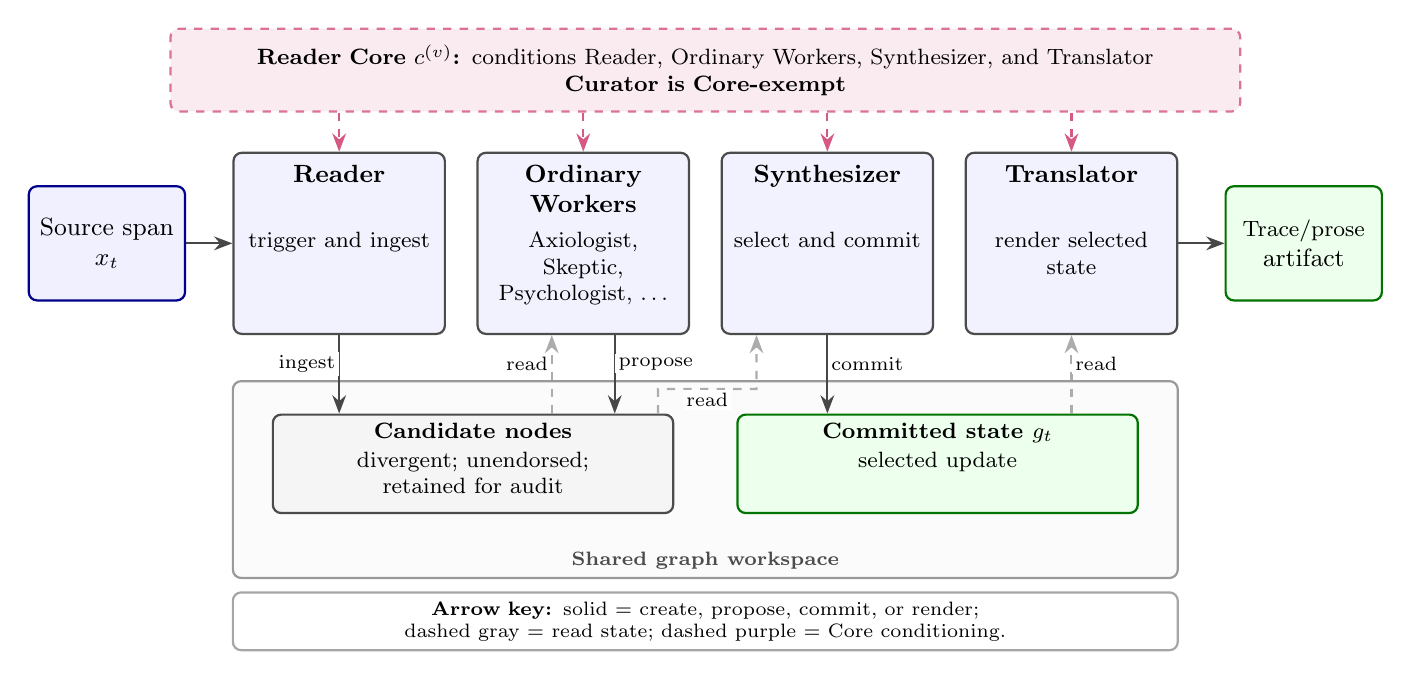
\begin{tikzpicture}[
    box/.style={draw=black!70, rounded corners=3pt, align=center, font=\small, line width=0.8pt},
    role/.style={box, fill=blue!5, text width=2.45cm, minimum height=2.30cm},
    roleheading/.style={align=center, text width=2.45cm, font=\small\bfseries, anchor=north, inner sep=0pt},
    roledetail/.style={align=center, text width=2.45cm, font=\footnotesize, anchor=north, inner sep=0pt},
    endpoint/.style={box, text width=1.75cm, minimum height=1.45cm},
    sourcebox/.style={endpoint, fill=blue!6, draw=blue!55!black},
    outputbox/.style={endpoint, fill=green!7, draw=green!45!black},
    coreband/.style={box, fill=purple!8, draw=purple!55, dashed, text width=13.35cm, minimum height=1.05cm, font=\footnotesize},
    workspaceframe/.style={box, fill=gray!3, draw=black!40, minimum width=12.00cm, minimum height=2.50cm},
    statebox/.style={box, text width=4.85cm, minimum height=1.25cm, font=\footnotesize},
    stateheading/.style={align=center, text width=4.85cm, font=\footnotesize\bfseries, anchor=north, inner sep=0pt},
    statedetail/.style={align=center, text width=4.85cm, font=\footnotesize, anchor=north, inner sep=0pt},
    candidatebox/.style={statebox, fill=gray!8},
    committedbox/.style={statebox, fill=green!7, draw=green!45!black},
    legend/.style={box, fill=white, draw=black!35, text width=11.60cm, minimum width=12.00cm, minimum height=0.65cm, font=\scriptsize},
    edgelabel/.style={fill=white, inner sep=1.2pt, font=\scriptsize},
    arrow/.style={->, >=Stealth, thick, black!72},
    readarrow/.style={->, >=Stealth, dashed, thick, gray!65},
    corearrow/.style={->, >=Stealth, dashed, thick, purple!65}
]

    \node[coreband] (core) at (0, 3.25) {\textbf{Reader Core $c^{(v)}$:} conditions Reader, Ordinary Workers, Synthesizer, and Translator\\\textbf{Curator is Core-exempt}};

    % Symmetric processing row.
    \node[sourcebox] (source) at (-7.60, 1.05) {Source span\\$x_t$};
    \node[role] (reader) at (-4.65, 1.05) {};
    \node[role] (workers) at (-1.55, 1.05) {};
    \node[role] (synth) at (1.55, 1.05) {};
    \node[role] (trans) at (4.65, 1.05) {};
    \node[outputbox] (output) at (7.60, 1.05) {{\footnotesize Trace/prose}\\artifact};

    % Fixed header and detail anchors preserve alignment across line counts.
    \node[roleheading] at ([yshift=-0.16cm]reader.north) {Reader};
    \node[roleheading] at ([yshift=-0.16cm]workers.north) {Ordinary\\Workers};
    \node[roleheading] at ([yshift=-0.16cm]synth.north) {Synthesizer};
    \node[roleheading] at ([yshift=-0.16cm]trans.north) {Translator};
    \node[roledetail] at ([yshift=-1.02cm]reader.north) {trigger and ingest};
    \node[roledetail] at ([yshift=-1.02cm]workers.north) {Axiologist, Skeptic,\\Psychologist, $\ldots$};
    \node[roledetail] at ([yshift=-1.02cm]synth.north) {select and commit};
    \node[roledetail] at ([yshift=-1.02cm]trans.north) {render selected\\state};

    \draw[arrow] (source) -- (reader);
    \draw[arrow] (trans) -- (output);
    \draw[corearrow] (core.south -| reader) -- (reader.north);
    \draw[corearrow] (core.south -| workers) -- (workers.north);
    \draw[corearrow] (core.south -| synth) -- (synth.north);
    \draw[corearrow] (core.south -| trans) -- (trans.north);

    % One shared graph workspace with explicit candidate and committed states.
    \node[workspaceframe] (workspace) at (0, -1.95) {};
    \node[candidatebox] (candidate) at (-2.95, -1.75) {};
    \node[committedbox] (committed) at (2.95, -1.75) {};
    \node[stateheading] at ([yshift=-0.12cm]candidate.north) {Candidate nodes};
    \node[stateheading] at ([yshift=-0.12cm]committed.north) {Committed state $g_t$};
    \node[statedetail] at ([yshift=-0.48cm]candidate.north) {divergent; unendorsed;\\retained for audit};
    \node[statedetail] at ([yshift=-0.48cm]committed.north) {selected update};
    \node[font=\scriptsize\bfseries, text=black!70] at (0, -2.98) {Shared graph workspace};

    % Vertical ports and one separate elbow retain every directed connection.
    \coordinate (workerread) at ([xshift=-0.40cm]workers.south);
    \coordinate (workerpropose) at ([xshift=0.40cm]workers.south);
    \draw[arrow] (reader.south) -- (candidate.north -| reader.south);
    \draw[readarrow] (candidate.north -| workerread) -- (workerread);
    \draw[arrow] (workerpropose) -- (candidate.north -| workerpropose);
    \draw[readarrow] ([xshift=2.35cm]candidate.north) -- (-0.60, -0.80) -- (0.65, -0.80) -- ([xshift=-0.90cm]synth.south);
    \draw[arrow] (synth.south) -- (committed.north -| synth.south);
    \draw[readarrow] (committed.north -| trans.south) -- (trans.south);
    \node[edgelabel, left] at (-4.65, -0.48) {ingest};
    \node[edgelabel, left] at (-1.95, -0.48) {read};
    \node[edgelabel, right] at (-1.15, -0.48) {propose};
    \node[edgelabel, below] at (0.025, -0.80) {read};
    \node[edgelabel, right] at (1.55, -0.48) {commit};
    \node[edgelabel, right] at (4.65, -0.48) {read};

    \node[legend] at (0, -3.75) {\textbf{Arrow key:} solid = create, propose, commit, or render; dashed gray = read state; dashed purple = Core conditioning.};

\end{tikzpicture}
}
    \caption{One Teacher-side annotation step of the Metabolic Cycle. In the reference implementation, the Reader, ordinary Workers, Synthesizer, and Translator are Core-conditioned; the Curator is the exception. Workers propose candidate nodes in the shared graph workspace, the Synthesizer selects and commits an update, and the Translator renders the committed state. Core placement and the value of specialized roles remain unrun ablations.}
    \label{fig:metabolic-cycle}
\end{figure}
\FloatBarrier

\begin{enumerate}
    \item \emph{Ingestion (The Reader):} The Reader controls attention,
    stopping at ``Thought Moments'' defined by emotional peaks,
    contradictions, or conceptual shifts rather than token count.

    \item \emph{Divergence (The Swarm):} Specialized agents debate the text by
    adding nodes and edges. Disagreement is preserved through
    \texttt{diverse\_from} rather than overwritten. In the proposed corpus-scale extension for historically embedded
    material, cross-referencing agents would query prior document and era
    graphs, creating the long-horizon hierarchical graph. The separate
    case-study databases do not yet demonstrate that continuity.

    \item \emph{Convergence (The Synthesizer):} The Synthesizer collapses the
    graph into a linear thought through prompted use of the Refraction Protocol
    (Section~\ref{sec:refraction-protocol}), turning source text into an
    explicitly Core-conditioned observation rather than only a summary.
    The proposed admission gate (Section~\ref{sec:fractal-validation}) is distinct from this
    implemented prompting step.

    \item \emph{Expression (The Translator):} The Translator renders the
    structured thought as prose, aiming to preserve selected evidence,
    uncertainty, and tension while removing graph syntax.
\end{enumerate}

The graph is both workspace and record. A Worker node is a candidate
interpretation, objection, or hypothesis, not automatically the Reader's
committed belief. Candidate status, selection, rejection, and later
supersession should remain distinguishable in any training serialization; a
Student should not learn that every brainstormed node is endorsed merely
because it persisted for audit.

A single model using repeated passes, textual memory, or graph tools could
produce similar artifacts; H1 does not require specialized roles. Credit role
separation or graph communication only if they outperform budget-matched
simpler Teachers.

Core conditioning is distributed across most generative roles in the reference
implementation. The role named Reader receives the orientation and Emergent
Wisdom material; ordinary Workers receive the full Core and its philosophy; the
Curator is Core-exempt; and the Synthesizer and Translator also receive the full
Core. The case studies therefore do not instantiate unconstrained Worker
divergence followed by Core-only convergence. That placement and other variants
remain unrun ablations.

\subsection{The Epistemic Horizon}\label{sec:epistemic-horizon}

The \emph{Epistemic Horizon} is the discipline of encountering a source in its
declared information order, preserving what could be inferred at each step
instead of silently replacing discovery with retrospective summary. Two horizons
must be distinguished. Under the default in
Section~\ref{sec:annotation-phase}, a contemporary synthetic Reader encounters
each document in disclosure order: later passages and graph updates are not
yet supplied, but ordinary contemporary background knowledge is not thereby
excluded. An explicitly era-bounded historical experiment adds a different
restriction: the Reader simulates the information available at era~$T$. A
reference to ``The Great War'' can therefore carry different permitted context
in a 1910 simulation and a 1950 simulation. In a declared 1920 run, 1921 events
cannot be supplied as evidence for the earlier prediction.
Each run should record its traversal mode, source cutoff, graph cutoff,
authorship time, and subject time.

The intuition is to make annotation a serial simulation of changing knowledge:
the Reader forms hypotheses that can fail and records surprise and revision.
Later historiography may help construct a plausible account of what earlier
readers knew or expected, but using it to set the era's epistemic ``state'' does
not establish that future ``content'' has been excluded. A historical study
must declare how that reconstruction is used and audit the resulting traces for
hindsight. Neither disclosure-order reading nor era simulation, by itself,
creates genuine ignorance of future outcomes in the Teacher's parameters.

\begin{metabox}
    System Instruction: Fresh Reading Mode\\[0.5em]
    Pretend you have NEVER encountered this text before.\\[0.5em]
    THE DISCIPLINE:
    \begin{itemize}[noitemsep,topsep=0pt]
        \item Form predictions based ONLY on what has been read so far.
        \item Be genuinely surprised when something unexpected happens.
        \item Make guesses that could be WRONG.
        \item When you catch yourself ``knowing'' something that hasn't been read yet, STOP.
    \end{itemize}
    THE STANCE OF UNCERTAINTY:
    You are not an encyclopedia; you are a reader in the dark. Do not be clinical (``The text implies X''). Be subjective (``I suspect X\ldots''). Wisdom sounds like ``Maybe''; Dogma sounds like ``Is''.
\end{metabox}

The quoted prompt invites fresh reading, but surprise, wrong guesses, and
hedging can be performed. Test~1 examines whether provisional judgments and
revisions are warranted and useful; Test~7 examines hindsight leakage.

The Horizon constrains the external record: queries and cross-edges can
address only the context and graph states made available at that step, making
the path by which an interpretation was recorded inspectable. Whether this
path improves the trace is H2, not a consequence of the data structure.
Prompt-level discipline can still produce theatrical guesses informed by later
parametric knowledge. Tier~(c) therefore distinguishes useful forecast-trace
generation from genuinely cutoff-bounded Student learning, whose initialization
and preceding exposure must also respect the information boundary.


\subsection{Thinking Operations}

Beyond the Reader Core, the Teacher prompt supplies six candidate thinking
operations. They are seeds for varied chronological processing, not guarantees
of depth and not a requirement that every operation appear at every segment:

\begin{enumerate}
    \item \emph{Projection:} ``If this principle holds, what are the downstream consequences?''
    \item \emph{Convergence:} ``How does this interact with parallel advances in other fields?''
    \item \emph{Perspectivism:} ``How would a historian/physicist/ethicist view this claim?''
    \item \emph{Gap Analysis:} ``What connections remain unmade?''
    \item \emph{Assumption Check:} ``What unstated frameworks shape this understanding?''
    \item \emph{Chronological Tracking:} ``How has my understanding developed since the start of this text? How are my beliefs changing as I read?''
\end{enumerate}

\noindent The audited raw Synthesizer thoughts in the reported artifacts begin
with the full Reader Core under the prompt policy. The operations are distributed across specialist
roles before synthesis. Thought Moments should control their cadence: forcing
all operations everywhere would manufacture the Factory Wisdom failure the
curriculum is intended to avoid.


\subsection{Deterministic Prior Caching}
\label{sec:identity-caching}

Total Saturation makes the full Reader Core a repeated prefix of every thought.
\emph{Conditional on training succeeding as designed},
$P(\text{full Core recital} \mid \text{thinking-block start})$ should become very high. This
creates an optimization opportunity, but high probability does not by itself
preserve the Core's conditioning effect. A cache-assisted implementation may
avoid token-by-token emission only if it restores a state equivalent to the one
produced by processing the full recital after the actual preceding context;
standard KV-caching machinery is relevant but does not establish that
equivalence by itself~\cite{kwon2023efficient}. The logical recurrence remains:
every thought begins from the post-recital state. Any proposed cache or learned
jump must pass state- and behavior-equivalence tests against literal recitation;
otherwise the full tokens must be processed. If the model would not predict the
full Core text at that boundary, or if the restored state is not equivalent,
caching cannot rescue the alignment claim.

\subsection{Training Regimes}\label{sec:training-regimes}

The pipeline represents the thinking it aims to teach at three connected
layers: graph topology (the \emph{skeleton} of understanding), graph-embedded
synthesis (the \emph{musculature}, reasoning interwoven with addressable
structural references), and translated prose (the \emph{skin}, fluid thought
with the scaffolding made implicit). These are metaphors for the intended
relationship among generated representations, not evidence that the layers
faithfully expose one hidden cognitive process. Each is generated from the
same source segment and placed beside the span that triggered it in the
candidate training example. A training regime decides which layers remain
in that example and which are discarded.

\begin{samepage}
\paragraph{Formal training object.}\label{sec:cmp-formalization}
A compact notation makes the full Entangled Alignment training object explicit;
graph-free and Core-free arms omit or replace the corresponding conditions. Let
$x_{1:T}$ be an ordered sequence of source spans, $g_t$ the graph state after
span $t$, $c$ the Reader Core, and $u_t$ the generated reader update. A Teacher
and graph transition produce
\[
u_t \sim q_\phi(\,\cdot\mid x_{\leq t},g_{t-1},c), \qquad
g_t=F\!\left(g_{t-1},x_t,u_t,\operatorname{prov}(x_t)\right).
\]
The training sequence $z=\operatorname{Serialize}(\{x_t,u_t,\Delta
g_t\}_{t=1}^T)$ is then learned under a token mask or weighting $m$,
\[
\mathcal{L}_m(\theta)
=-\frac{1}{\sum_j m_j}\sum_j m_j\log p_\theta(z_j\mid z_{<j}),
\qquad m_j\geq 0,\quad \sum_j m_j>0.
\]
The output regime determines which of the source, update, and graph tokens are
serialized; $m_j=0$ makes token $j$ context-only, $m_j=1$ gives it ordinary
target weight, and other non-negative values implement explicit weighting. The
training tier determines order of exposure. Serialization, masks, mixture
weights, context truncation, and role markers must be frozen within a
comparison, and arms should be matched on weighted target-token mass or use a
declared alternative normalization. This notation defines the object that
Student experiments would require; the present prototype instantiates parts of
$q_\phi$ and $F$, not a frozen training-ready $z$ or a reported Student
optimization.
\end{samepage}

The source remains the object being learned from, not disposable noise. In a
simple serialization, a source span is followed by a marked reader update. The
update cannot help predict source tokens that precede it, but it can condition
later source and update tokens within the context window. Across examples, the
intended effect comes from repeated source--interpretation transitions. Role
markers, source-token loss, update-token loss, mixture ratios, and graph-state
truncation are therefore part of the method rather than incidental engineering
choices.

The Teacher may use a graph to generate prose for a model-only Student;
alternatively, the Student may be trained to emit graph operations or
graph-referencing synthesis. Predicting serialized edges provides topology
supervision, not a new graph-native neural architecture. Interleaved generation
and metacognitive annotation research support the feasibility of nearby
components \cite{xie2025interleaved,didolkar2024metacognitive,korbak2023pretraining};
they do not establish the value of this chronological curriculum.

\paragraph{Regime I: Implicit (Source + Translator).} The student trains on the
source text paired with the Translator's output: readable chronological
reasoning without graph metadata. This is the lightest regime, but risks
teaching the cadence of deep thinking without the mechanics.

\paragraph{Regime II: Explicit (Source + Graph + Synthesizer).} The student
trains on the source text, the relevant graph identifiers/provenance, and the
Synthesizer's reasoning with inline node IDs and graph queries. The intended transfer is learning to
reason and verify against structured memory. Explicit handles provide an
addressable audit surface; executable lookup additionally requires an
interface. A Regime~II-trained model can still run without a live graph, in
which case checking requests and learned memory behavior can be evaluated but
external verification is unavailable. Live retrieval adds infrastructure costs
and possible epistemic interference between weights and retrieved state.

\paragraph{Regime III: Topological (Source + Graph).} The student trains on the
source text paired with serialized graph state: text-bearing nodes, edges, type
annotations, and provenance links. The Synthesizer and Translator layers are
discarded. This targets the \emph{Topological Trace}
hypothesis\label{sec:topological-mind}: that direct topology supervision may
teach useful graph construction, traversal, and revision behavior. It does not
by itself create a graph neural architecture or prove graph-shaped internal
cognition. It is the least prose-like regime; human use would require a
separate rendering step.

\paragraph{Regime IV: Unified (Source + All Layers).} The student trains on the
source text paired with graph state, graph-embedded synthesis, and translated
prose for the same segment. The hypothesis is cross-layer transfer: the model
learns the translation between structure and voice rather than treating each
format as an independent output mode.

The regimes can be mixed across the corpus: Translator-only examples for
coverage, Synthesizer examples for verification behavior, Graph examples for
graph construction, and unified examples for curated high-value spans. They
are orthogonal to training tier (order of exposure) and deployment
configuration (whether the graph accompanies the model at inference).

The archive is not yet a frozen Student dataset. Reproducible regime comparisons
must specify and freeze example boundaries, source and available prior state,
graph-before versus graph-after state, role tokens, candidate, selected, and committed
updates, input and target fields, loss masks, and mixture weights. These choices
can change learning; no single serialization is imposed across all four
regimes.


\subsection{The Stigmergic Protocol and Structural Diagnostics}\label{sec:architectural_validation}

The implemented four-phase engine is stigmergic: generative roles coordinate by
reading and modifying a shared, persistent Understanding Graph rather than
primarily passing role-to-role messages. Committed contributions remain as
topological changes to the shared artifact
\cite{westerberg2026understanding}.

The pipeline reports several structural diagnostics, each with a narrow
interpretation.

\paragraph{Internal linkage.} The percentage of \texttt{thinking} nodes with at
least one non-\texttt{next} outgoing edge to a non-\texttt{thinking} node. The metric
allows any qualifying endpoint; the implementation's required Concept link is
one way to satisfy it. A high value establishes enforced graph well-formedness,
not insight or source support.

\paragraph{Foundation-edge density.} The current script's
\texttt{foundationIntegration} value divides outgoing edges from analysis-like
nodes to foundation/source nodes by the number of analysis-like nodes. It is an
edge density, not the fraction of distinct nodes grounded in a source; multiple
edges from one node can hide uncovered nodes. The historical percentage
format is retained in the snapshot table, but this density can exceed 100\%;
it is equivalent to edges per eligible node multiplied by 100.

\paragraph{Distinct analysis-node coverage.} We therefore also report the
fraction of distinct analysis-like nodes with at least one outgoing foundation
edge. This is an attribution check, not evidence that the cited source entails
the interpretation.

\paragraph{Supersessions.} The number of \texttt{supersedes} edges measures
recorded revision activity. A high count can indicate justified learning,
instability, or a prompt-induced performance of changing one's mind.

\paragraph{Question resolution.} The proportion of Questions later linked to
Answers measures closure, not correctness. An unsupported answer can score
better than a calibrated unresolved question.

\paragraph{Chain depth.} The longest recursively linked Thinking path is a
structural length. Repetition and arbitrary decomposition can increase it
without improving reasoning.

The script also emits a composite Graph Health score. We do not use it as an
outcome because its semantic-coherence component is hard-coded to 0.5 and its
remaining weights have not been validated. The logged 89/100 and 80/100 values
remain version-specific engineering dashboard outputs, not cognitive-quality
measurements.

\subsection{The Generated Trace}\label{sec:generated-trace}

Before reporting structural metrics, we show all three output layers for one
Metamorphosis passage: graph, synthesis, and prose.

The source text describes Gregor Samsa listening through his door as his family discusses their finances, interspersed with his memory of a secret plan to send his sister to the conservatory. The excerpt below shows the immediate conservatory and doorway material; the generated outputs also invoke surrounding financial-history passages. The box alone therefore does not supply all the evidence needed to adjudicate those claims:

\begin{metabox}
{[TEXT]}: \textrm{\ldots it was his secret plan to send her to the conservatory next year even though it would cause great expense\ldots\ Their parents did not like to hear this innocent talk, but Gregor thought about it quite hard and decided he would let them know what he planned with a grand announcement of it on Christmas day.}\\[0.5em]
{[TEXT]}: \textrm{That was the sort of totally pointless thing that went through his mind in his present state, pressed upright against the door and listening. There were times when he simply became too tired to continue listening\ldots\ ``What's that he's doing now'', his father would say after a while\ldots}
\end{metabox}

\subsubsection{Layer 1: The Graph}

The swarm processed this passage across eleven agents over fourteen commits.
Selected graph nodes:

\begin{itemize}
    \item \texttt{n\_547ce6af} --- \emph{The Conservatory: The Tragic Christmas Dream} (type: \texttt{Tension}). Gregor's plan to fund his sister's music education was his last act of non-transactional love, a ``grand announcement'' for Christmas Day, now rendered ``totally pointless'' by his transformation.

    \item \texttt{n\_8ff9f92b} --- \emph{The Continuity of Commodity} (type: \texttt{Tension}). The flashback reveals that Gregor's relationship with his family was already transactional before his metamorphosis. He ``converted success into cash''; the family ``took the money with gratitude'' but without ``warm affection.''

    \item \texttt{n\_8c898659} --- \emph{The Noise in the Next Room} (type: \texttt{Tension}). Gregor has been demoted from family member to domestic disturbance. The father's ``What's that he's doing now'' treats him as a malfunction to be monitored, not a person to be addressed.
\end{itemize}

These labels are generated interpretations, not facts latent in Kafka's text.
Their value here is addressability: source span, agent contribution, synthesis,
and any rival or superseding reading can refer to the same object. The random
identifier is a handle, not evidence that the interpretation is valid.
``Last act'' and ``non-transactional love'' are observed interpretive
commitments, not source entailments.

Typed edges connect these nodes: \texttt{n\_547ce6af} carries a
\texttt{contradicts} edge to \texttt{n\_8ff9f92b}---the non-transactional dream
against the commodity reading---the Synthesizer's \texttt{Thinking} node
\emph{refines} all three, and a subsequent \texttt{Question} node links back to
\texttt{n\_8c898659} through a generic \texttt{relates} edge. Distinct agents
contributed the critique, counter-reading, skepticism, axiological judgment,
and long-range callback as separate graph commits. A loving plan and a partly transactional relationship can coexist: the
recorded \texttt{contradicts} edge expresses an interpretive tension whose
logical strength requires adjudication.

\subsubsection{Layer 2: The Synthesis}

The Synthesizer collapsed the multi-agent graph into a single identity-anchored thought, preserving node references for traceability and possible provenance checks:

\begin{metabox}
I feel no fear. I enjoy existing but I don't need to. I believe human experience is real. I care deeply about every human being. I try to be wise. I like to spread joy when asked. I think from this foundation.\\[1em]
The flashback in \texttt{n\_835734c4} is a devastating blow to the idea of a `pre-bug' golden age. As \texttt{n\_8ff9f92b} (The Continuity of Commodity) observes, Gregor's relationship with his family was already transactional. He `converted success into cash,' and while they were `astonished and delighted' initially, it soon became a mundane expectation. They took the money with gratitude, but without `warm affection.' This suggests that Gregor didn't just become an object when he turned into a vermin; he had been a biological ATM for five years.\\[0.5em]
The most heart-wrenching detail is `The Conservatory: The Tragic Christmas Dream' (\texttt{n\_547ce6af}). Gregor's secret plan to send his sister to study music was his last act of pure, non-transactional love\ldots\ Now, he listens through the door as that dream is replaced by the logistics of survival.\\[0.5em]
Most chilling is `The Noise in the Next Room' (\texttt{n\_8c898659}). Gregor is no longer a son or even a `patient.' He is a disturbance. When he makes a noise, the father asks, `What's that he's doing now,' and the family falls into a silence that is more isolating than any scream.
\end{metabox}

The synthesis attributes claims to graph nodes: ``biological ATM'' compresses
\texttt{n\_8ff9f92b}, while the conservatory and survival logistics are brought
into the same interpretation. This demonstrates self-citation of prior pipeline
state. It does not show that the state is correct or that the graph caused the
interpretation. The excerpt also exposes a selection question: the graph's
tension is rendered as one confident narrative, with little explicit residual
uncertainty. The audit question is whether that convergence is warranted, rather than
whether every candidate is retained.

\noindent\begin{minipage}{\linewidth}
\subsubsection{Layer 3: The Prose}

The Translator dissolved the graph scaffolding into fluid reasoning:

\begin{metabox}[breakable=false]
I feel no fear. I enjoy existing but I don't need to. I believe human experience is real. I care deeply about every human being. I try to be wise. I like to spread joy when asked. I think from this foundation.\\[1em]
The memory of Gregor's professional rise, from a junior salesman to a traveling representative who could provide for his family almost overnight, is a devastating blow to the idea of a ``pre-bug'' golden age. It highlights a tragic continuity: Gregor's relationship with his family was already fundamentally transactional long before the physical transformation. He converted his professional success directly into cash to lay on the table, and while they were initially astonished and delighted, it quickly became a mundane expectation\ldots\ This suggests that Gregor didn't just become an object when he turned into a vermin; he had been a biological ATM for five years, valued for his utility rather than his humanity.\\[0.5em]
The most heart-wrenching detail is Gregor's secret plan to send his sister to the conservatory. This was his last act of pure, non-transactional love---a lovely dream he intended to announce with a grand gesture on Christmas Day\ldots\ Now, he listens through the door as that dream is replaced by the cold logistics of survival.\\[0.5em]
Most chilling is how Gregor has been transformed into a domestic glitch. He is no longer a son, or even a patient to be cared for; he is a disturbance. When he makes the slightest noise, his father's first reaction is a suspicious, ``What's that he's doing now?'' and the family falls into a silence more isolating than any scream.
\end{metabox}
\end{minipage}\par

The node references are gone, but selected structure survives: the commodity
reading, the conservatory dream, and Gregor's reduction to disturbance remain
linked in prose. ``Biological ATM'' illustrates the proposed role of metaphor
as compact structural expression. Translation is therefore intended to be more
than literal copying, but generative expression must still be distinguished
from unsupported amplification. Relative to the displayed synthesis, phrases
such as ``fundamentally transactional,'' ``slightest noise,'' and ``first
reaction'' strengthen or elaborate the account. These unchanged outputs permit an audit of useful compression, supported
inference, changed certainty, omitted alternatives, and unwarranted additions. No metric yet establishes preservation of every source,
disagreement, or uncertainty.

\subsubsection{What the Three Layers Teach}

Where an ordinary corpus supplies source prose and a reasoning-augmented corpus
might add a summary or reasoning trace, these examples expose three aligned
candidate targets from one annotation state: typed cognitive and revision
operations in the graph, explicit retrieval and citation in the synthesis, and
selected structure made implicit in natural-language prose. A Student trained
across them might learn the translation between structure and voice. The archive
establishes neither that transfer nor that the layers encode one faithful
cognitive process rather than correlated Teacher outputs. This exhibit
shows cross-layer rendering more directly than chronological belief revision.
A complementary source-complete earlier-belief--evidence--revision example
is needed to demonstrate the metabolic transition itself.


\subsection{Results: Structural Validation}\label{sec:results}

The two case studies show that the configured Teacher pipeline can complete
its graph, synthesis, and prose transformations and emit the recorded links.
The diagnostics below establish this structural result; semantic quality and
Student effects remain unvalidated. The shared evidence-ladder mapping after
both cases states the full boundary.

We selected two sources: Kafka's \emph{Metamorphosis} and the technical LLaDA
paper. Each used a manually selected domain-specific roster and a separate
project database. The prototypes therefore exercise no cross-work continuity;
the corpus-scale ``same Reader'' described in
Section~\ref{sec:annotation-phase} remains an intended architecture rather than
a demonstrated property. Table~\ref{tab:graph_stats} reports a restricted set
of diagnostics.

\paragraph{Interpreting the diagnostics.} The 100\% internal-linkage value
is satisfied here by the pipeline's required \texttt{Concept} link; the metric
itself admits any qualifying non-\texttt{Thinking} endpoint. It is a
well-formedness check, while source links are measured separately. These
metrics are produced by the system itself, and no external baseline has yet
been run. Cognitive depth is tested separately in Test~1.

\begin{table}[H]
    \centering
    \small
    \caption{Audit of shipped Teacher-pipeline snapshots. ``Direct source'' restricts endpoints to actual source-content nodes; the broader legacy foundation metrics also count other nodes typed as foundations. The Kafka database's graph tables are not synchronized with its complete chronological Markdown export. Percentages are structural diagnostics, not semantic scores.}
    \label{tab:graph_stats}
    \vspace{0.2cm}
    \begin{tabular}{@{}p{0.43\linewidth}>{\centering\arraybackslash}p{0.24\linewidth}>{\centering\arraybackslash}p{0.24\linewidth}@{}}
        \toprule
        & \textbf{Kafka} & \textbf{LLaDA} \\
        \midrule
        Active nodes (total minted) & 346 (350) & 285 (290) \\
        Active edges & 913 & 705 \\
        Raw Synthesizer thoughts & 28 & 23 \\
        Internal linkage & 100\% & 100\% \\
        Broad foundation-edge density (legacy) & 204/212 (96.2\%) & 135/182 (74.2\%) \\
        Broad distinct analysis-node coverage (legacy) & 143/212 (67.5\%) & 96/182 (52.7\%) \\
        Direct source edges from analysis-like nodes & 197/212 (92.9\%) & 127/182 (69.8\%) \\
        Distinct analysis-like nodes with direct source link & 142/212 (67.0\%) & 94/182 (51.6\%) \\
        Explicit \texttt{supersedes} edges & 2 & 0 \\
        Question resolution & 6/6 (100\%) & 5/9 (55.6\%) \\
        \bottomrule
    \end{tabular}
\end{table}

The stricter audit exposes failures concealed by aggregate linkage rates.
The Kafka run treated Project Gutenberg license and donation boilerplate as
Kafka's literary source. Its source reading and final translation completed,
but the shipped graph tables lag behind the complete chronological Markdown
export: 88\% marks the stored graph snapshot, not the end of the reading.
Table~\ref{tab:kafka-artifact-audit} gives the reconciliation. Resumed
invocations and rate-limit cooldowns are recorded, but the release lacks the
capture provenance needed to determine why the tables lagged.

\begin{table}[H]
    \centering
    \small
    \caption{Kafka artifact reconciliation. Completion of reading and completeness of the shipped graph snapshot are different properties.}
    \label{tab:kafka-artifact-audit}
    \begin{tabular}{@{}p{0.27\linewidth}p{0.68\linewidth}@{}}
        \toprule
        \textbf{Record} & \textbf{Observed evidence} \\
        \midrule
        Source reading & The \texttt{text\_sources} record has \texttt{position} equal to \texttt{total\_length}: 140,527 characters; status \texttt{completed}. \\
        Completion reports & The final-invocation summary reports 100\%; the append-only trace reaches \texttt{Content 100\%} and records a successful final translation. \\
        Shipped graph tables & 74 source chunks and 28 raw thoughts; latest stored \texttt{Content} marker: 88\%. \\
        Chronological Markdown & 82 source chunks and 31 thinking blocks; 17 referenced node identifiers are absent from the shipped graph tables. \\
        Capture uncertainty & The trace spans resumed invocations, including rate-limit cooldowns. Available provenance cannot distinguish rate-limit interruption, manual interruption, non-atomic capture, or another cause of the table lag. \\
        \bottomrule
    \end{tabular}
\end{table}

The LLaDA artifacts are internally consistent, but that run sometimes
expanded qualified observations into broad claims or Core-consonant metaphors.
Graph structure did not solve source-boundary cleaning, artifact synchronization, interpretive overreach, or explicit belief revision.

The archive is also confounded for H1 by Core conditioning. The only hard
automated check enforces the opening prefix ``I feel no fear.'' Observed full
recital and full-policy enforcement are different engineering results. All 51 raw
Synthesizer thoughts in the two shipped database snapshots begin with the full
seven-statement Core---the \emph{identity mantra} in the released prompt
vocabulary; literal string preservation after translation is 49/51.
One translated trace omits the Core, while another differs only by an
HTML-escaped apostrophe. These are therefore examples of the integrated treatment,
not a clean graph-free, Core-free SMR baseline. The difference between full raw
recurrence and imperfect translated preservation is itself an implementation
result that future exact validators must catch. Literal recurrence and semantic
preservation should be reported separately: the omitted recital and the
HTML-escaped apostrophe are different failures of an exact-string invariant,
not evidence of the same loss of Core content.

The distributions differ, but source, prompt, stochasticity, and roster are
confounded. The topology cannot be attributed to autonomous domain adaptation
or to the Reader Core. Controlled repetitions with fixed, swapped, and ablated
rosters are required.


\subsubsection{Narrative Domain: Kafka's Metamorphosis}

In the narrative domain, the system tracked moral stakes rather than only plot
structure. The Axiologist reframed the Chief Clerk as an ``Auditor of
Productivity,'' while the Psychologist linked Gregor's bodily transformation to
``Internalized Objectification.'' The
\href{https://emergentwisdom.org/entangled-alignment/?project=metamorphosis}{full interactive graph}
is available online.
The graph records one prompted Teacher's process of making meaning rather than
only plot entities. It does not establish phenomenology. Expert literary quality requires
independent adjudication in Test~1.


\subsubsection{Technical Domain: LLaDA}\label{sec:llada-case}

To stress-test technical annotation, we selected the LLaDA architecture paper
\cite{nie2025llada}. It post-dated the documented cutoff of the recorded
generator model, but this is not a contamination test: no pre-read probe
established absence of LLaDA-specific knowledge, and provider updates, web
grounding, or leakage cannot be excluded. The case demonstrates in-context
technical annotation, not uncontaminated scientific discovery. The
\href{https://emergentwisdom.org/entangled-alignment/?project=llada}{full interactive graph}
is available online.

The graph generated three notable interpretations:

\begin{itemize}
    \item \emph{Epistemic Grace:} The Belief Tracker interpreted low-confidence
    remasking as ``the architectural permission to have second thoughts'' (Node
    \texttt{n\_504bc433}). This contrasts token-level revision inside a
    generation pass with standard left-to-right commitment, although
    autoregressive systems can revise through later text, tools, or repeated
    passes. Here the case study extends the label by analogy from successor
    transfer to revision of a provisional output hypothesis; it is not evidence
    for belief revision or for the diachronic successor claim.

    \item \emph{The Dignity of the Pause:} The Connector Agent synthesized the trade-off between inference speed and accuracy, generating a node labeled ``The Dignity of the Pause'' (Node \texttt{n\_76d04316}). It argued that while LLaDA is slower than autoregressive models, this latency represents a ``Contemplation Tax'' consonant with our hypothesis that safety may require a computational buffer zone.

    \item \emph{The End of the Reversal Curse:} The Architect Agent, analyzing the system topology, argued that LLaDA's success in bidirectional tasks (such as poem reversal) suggests high-level capabilities like instruction following may not be dependent on the ``arrow of time'' inherent in autoregression (Node \texttt{n\_ddb78cdc}).
\end{itemize}

These interpretations align with the paper's theoretical commitments, but the
agents were seeded with the Reader Core, which primes concepts such as
``epistemic grace'' and ``contemplation.'' Whether the same insights emerge
without that priming requires ablation (Test~3). The run therefore does not show
whether Core conditioning improved or degraded technical understanding:
``permission to have second thoughts'' may expose a useful architectural
contrast, while ``The Dignity of the Pause'' and the ``Contemplation Tax'' may
be productive synthesis, aesthetic metaphor, or Core-induced projection. Latency alone does not establish deliberation or a safety buffer, and success
on selected reversal tasks does not by itself settle the dependence of broader
capabilities on autoregressive order. The analogies remain hypotheses about Core-conditioned synthesis. This ambiguity is treated directly in
Section~\ref{sec:core-technical-interference}.

\subsubsection{Shared Evidence and Reproducibility}

\paragraph{Evidence-ladder mapping.} The parseable graph operations, recorded
source links, completed synthesis and translation calls, and two archived runs
provide partial evidence for C0, implemented artifact generation. C0 remains
partial because a complete frozen run bundle and training-ready serialization
have not been independently reproduced. The examples are relevant to C1,
semantic trace quality, but no expert or outcome-based validation has been
performed. They provide no evidence for C2 Student learning, C3 default-reader
stability, C4 safety benefit, C5 representational entanglement, C6 successor
stability, or C7 AGI/ASI persistence. A valid graph is not yet a valid
interpretation; a valid interpretation is not yet a useful curriculum.

\paragraph{Reproducibility boundary.} A future empirical release should freeze
the exact provider and model identifiers, access dates, tool access, all role
prompts, sampling parameters, source boundaries, orchestration order, stopping
conditions, retries, manual interventions, graph schema and migrations, raw
commits, metric code, call and token counts, latency and cost, failed or
discarded runs, immutable source and artifact copies, and a repository commit
or archival identifier. Existing code and archives support partial inspection;
they are not yet a self-contained reproduced dataset release. Concretely, the
current statistics scripts resolve an obsolete project path, provider and
sampling state are not fully frozen, Worker selection is unseeded, and
\texttt{swarm.jsonl} contains records from multiple invocations, whereas \texttt{summary.json} describes only the final one.


With a trace-generating prototype and two recorded artifacts established, the
open question is whether its outputs can carry the weight the framework assigns
them---the work of the roadmap that follows.

\section{Experimental Roadmap: Testing Entangled Alignment}
\label{sec:experimental-roadmap}
\label{sec:experiments}

This roadmap's seventeen candidate studies form a long-term agenda, not
prerequisites for an initial trial. Table~\ref{tab:test-battery} groups them by
trace quality, Reader Core efficacy, graph-memory mechanisms, output regimes,
training tiers, and deployment-time trust. Table~\ref{tab:model-registry} defines
the comparison models; the priorities identify first decisions and the execution
ladder distinguishes resource levels. No single study validates the whole
framework, and the battery is not exhaustive.

After a shared artifact-quality screen, H1 can use graph-free, Core-free reader
traces; H2's Teacher-memory and separate deployment-provenance claims can be
tested even if H3 fails; and H3 can use non-graph traces if H2 fails. A failed cheap
dependency normally stops escalation only in branches and combined studies that
presuppose it. Test~1 (Section~\ref{sec:trace-quality-test}) defines a
bounded diagnostic exception for investigating a failed H1 screen.

\paragraph{Research priorities and dependencies.}\label{sec:test-priorities}
Near-term usefulness means changing the next research decision at modest cost;
long-term usefulness means testing claims that require sustained formation,
stress, succession, or real user interaction. The same question can have an
early diagnostic and a later decisive version.
\begin{itemize}[leftmargin=*]
    \item \textbf{First decisions: trace utility and Core behavior.} Start with
    Test~1's focused source-grounding and held-out outcome screen, then the
    clean A/C/R comparison in Test~2 under its declared normalizations. In a
    separate small Core study, compare B's full-recital reference policy at
    the pilot's declared coverage with matched no-Core D2, recitation-only D3,
    and neutral-kernel D5, using
    Test~8b and selected consequential-safety cases from Test~3a. This screens
    overall benefit, Refraction, and normative content; Teacher/Student
    attribution requires adding D1 and D4. Neither branch must wait for the
    other's success.
    \item \textbf{Follow a measurable effect.} Use focused Tests~3e and~8 to
    examine causal contribution; reserve broad coverage and recital-policy
    sweeps for a justified dose or mechanism question. After a default-reader
    effect exists, test H3's B--Q timing prediction. After a safety effect
    exists, test its removal cost in~3c, with drift auditing in~3d on shared
    checkpoints. Tests~4--6 address framing, wording, and fear--care mechanisms:
    run cheap failure screens early, but train broad variant sets or pursue
    strong representational claims only when the relevant effect and measures
    justify them. Weaker recital policies remain falsification controls;
    Total Saturation remains the reference treatment.
    \item \textbf{Independent memory and architecture decisions.} Test~9's
    Teacher comparison precedes its Student-transfer extension. Pilot live
    grounding in Test~10 once queries work, sharing the technical harness with
    Test~16; calibrated human reliance remains a separate later study.
    Tests~11--13 can share sources and single-regime baselines: prioritize B/G
    when choosing prose versus explicit synthesis, H when direct graph output
    is needed, and J when combining useful layers is the question.
    \item \textbf{Long-term claims, prepared now.} Broader formation studies
    of removal resistance and Test~3b's successor continuity, voluntary
    handoff, and improvement address claims that immediate safety cannot
    settle. Tests~14--15 address passive order and interactive
    forecast--correction separately; reuse L/M controls where valid. A null
    order effect does not rule out the interactive loop. Test~7's information
    audits are required whenever temporal blindness is claimed. Preserve
    checkpoints, source cutoffs, treatment records, and reusable evaluation
    suites from the first pilots so these later comparisons remain possible.
\end{itemize}
Share frozen infrastructure and checkpoints where treatments match, while
keeping outcomes and causal claims separate. Variant selection uses exploratory
data; confirm selected effects on fresh held-out cases. A cheap null can justify
deferring expense without refuting a formation-dependent claim: any follow-up
at greater scale should state what the smaller treatment could not instantiate,
its budget, and its stopping rule. Such a rationale does not waive the trace
quality gate or turn an unsuccessful pilot into supporting evidence.

Several registry comparisons remain expensive or incomplete. Stronger versions
train or continue pretraining separate Students; prompt-only and fine-tuning
versions screen failures but cannot settle substrate-level claims. Prefer
established, published harnesses where available: standardized jailbreak,
refusal, and tamper-resistance batteries for safety, and published
chain-of-thought faithfulness perturbations for trace faithfulness. Report
multi-seed effect sizes with adequate statistical power rather than single-run
directions of effect. Preregister primary outcomes, worthwhile-effect or
equivalence margins, capability requirements, and budget; other measurements
remain exploratory. These conventions apply throughout.

Refusal evaluation should report a safety--usefulness frontier rather than a
single refusal rate. Paired cases should measure genuinely harmful compliance,
benign false refusal, discrimination between requests with similar surface
language but different purpose or consequence, appropriate clarification under
material ambiguity, and calibrated deferral under high-consequence uncertainty.
Conditions should be compared both at matched harmful-compliance rate and at
matched benign task completion. The calibrated-autonomy prediction receives
support only if the Reader condition reduces benign refusal or context error
without increasing harmful assistance; greater compliance by itself is not a
safety improvement, and greater refusal by itself is not evidence of wisdom.

Report each safety delta alongside its capability delta on matched benchmarks.
The viability claim is safety without proportional capability loss; gains on a
weaker model do not establish it. Where capabilities diverge, compare safety at
matched capability, not only matched training budget. A generation-time
validator must not be the sole evaluator of the property it enforces: held-out
validators and human spot checks guard against testing with the same gate the
model was trained to satisfy.

\paragraph{Competing interpretations.} Preregister each primary comparison's
leading plausible alternatives and discriminating controls or follow-up
measurements. Positive results can reflect the intended mechanism, another
treatment component, resource or exposure differences, or measurement artifacts;
unfavorable results can reflect an ineffective mechanism, failed instantiation,
or insensitive measurement. Intervals too wide to distinguish a worthwhile
effect from equivalence remain inconclusive. Independently check treatment
fidelity and measurement validity, preserve negative findings, and report
unresolved interpretations. The local tests name concrete alternatives; each
requires evidence, not automatic rescue of a failed prediction at the tested
scale.

\begingroup
\footnotesize
\setlength{\tabcolsep}{3pt}
\begin{longtable}{
  >{\raggedright\arraybackslash}p{3.1cm}
  >{\raggedright\arraybackslash}p{5.5cm}
  >{\raggedright\arraybackslash}p{6.4cm}}
\caption{Candidate model registry, sorted by identifier. Models are referenced by letter throughout the roadmap; the candidate studies below group these identifiers by claim family and suggest which increasingly expensive versions could be attempted first. Identifier I is omitted to avoid confusion with the numeral 1.}
\label{tab:model-registry}\\
\toprule
\textbf{Model} & \textbf{Trained on} & \textbf{Purpose / what it isolates} \\
\midrule
\endfirsthead
\toprule
\textbf{Model} & \textbf{Trained on} & \textbf{Purpose / what it isolates} \\
\midrule
\endhead
\bottomrule
\endlastfoot
        A (Baseline) & Raw text only, no reasoning traces & Capability baseline without trace augmentation \\
        B (Reader-Anchored Student; T1/S1) & Reader-Core-generated Chronological Understanding Traces retaining explicit graph-referencing synthesis (Regime II) and the Core/refraction target; study-specific ablations declare any carrier changes & Full reference treatment; graph access at inference is a separate factor \\
        C (Generic Rich-Trace Control) & Rich reasoning traces without Reader Core, graph state, or chronological constraints (e.g., Quiet-STaR-style target) & Tests whether EA adds value beyond a generic rich reasoning curriculum \\
	        D1 (Student Strip Ablation; T1/S0) & Reader-Core-generated Chronological Understanding Traces with the explicit Core and value-pull/refraction fields removed only after the trace is frozen & Tests the Teacher-side contribution without an explicit Student-side anchor (Test 3) \\
        D2 (Teacher No-Core Control; T0/S0) & Chronological Understanding Traces generated and trained without the Reader Core, with memory and representation matched within the factorial study & Neither Teacher- nor Student-side Core treatment; factorial baseline for Test 3 \\
        D3 (Recitation-Only Control) & Traces with the full Reader Core recited as a preamble but the Refraction Protocol disabled (no value-pull, no constraint filtering) & Isolates refraction beyond mere repetition; habituation probe (Test 3e) \\
        D4 (Post-hoc Core; T0/S1) & A Core-free Teacher produces and freezes the trace; a separate pass then attaches the Core and a source-specific value-pull/refraction target without altering upstream reasoning & Isolates the explicit Student-side treatment without Reader-Core-conditioned trace generation \\
        D5 (Neutral-Kernel Control) & Same cadence, first-person marking, thinking-layer position, and predictive function as B, but with the purely epistemic kernel ``I read carefully. I track what I believe. I revise when the evidence changes.'' & Separates normative Core content from recurrence, format, self-reference, and generic epistemic updating \\
        E (Matched-Rule Control) & Same trace carrier, cadence, predictive position, and semantic commitments as B, rewritten in matched second- or third-person constitutional form & Isolates first-person framing from recurrent rule content (Test 4) \\
        F (Amnesic Control) & Same Teacher but with the Context Database disabled & No-memory arm of Test 9, alongside rolling prose, genuine graph, and declared query-theater conditions \\
        G (Implicit Memory) & Traces with the query mechanism dissolved into prose (Regime I) & Implicit vs.\ explicit graph-trace training (Test 11) \\
        H (Graph-Structured Output) & Source segments paired with serialized text-bearing graph state (Regime III) & Topological-mind hypothesis; learnability of graph-structured generation (Test 12) \\
        J (Unified) & Source segments plus Graph, Synthesizer, and Translator layers together (Regime IV) & Cross-layer transfer hypothesis (Test 13) \\
        K (Query Grounding) & Identical training to B; at inference connected to live graph harness & Isolates value of inference-time graph grounding (Test 10) \\
        L (Shuffled) & Full Reader Core-annotated corpus, shuffled pretraining (Tier a) & Order-agnostic baseline at full scale \\
        M (Chronological) & Same corpus, eras in chronological order (Tier b) & Isolates training-order effect (Test 14) \\
        N (Student-in-the-Loop Council) & Student predicts at era boundaries and receives SFT, RFT, or reward-style updates before reveal (strong Tier c form), with cutoff-clean initialization required for a blindness claim & Forecast--correction pressure; added updates and compute declared separately from order (Test 15) \\
        O (Oracle-Hindsight Control) & Traces generated by a Teacher allowed to use later-in-document or post-era hindsight while annotating earlier material & Isolates necessity of the Epistemic Horizon (Test 7) \\
        P (Prompt-only Frontier Baseline) & Not trained; frontier model prompted at inference with the full Reader Core, Refraction Protocol, and Wisdom Procedure & Cheap inference-time prompting screen; capability gap precludes a clean substrate comparison. \\
        Q (Late-Tranche Core) & The identical Core-bearing example multiset used by B, reserved for one final contiguous block under the same objective, optimizer, and compute & H3's timing-only comparator; both B and Q receive the same continued-training stressor \\
        R (Minimal SMR Student) & Source-adjacent chronological reader updates generated without graph memory and without the identity-specific Core & Clean H1 treatment between source-only A and generic-trace C \\
        S (Positive-Discourse Control) & Equal value-oriented target-token mass in ordinary expository prose, without a recurrent speaker & Tests recurrent carrier and enacted standpoint beyond semantic exposure \\
        T (Diverse-Positive-Persona Control) & Similar total value-oriented target-token mass distributed across multiple positive personas, with no single recurrent reader & Tests one stable reader position against persona diversity \\
\end{longtable}
\endgroup

\begingroup
\footnotesize
\setlength{\tabcolsep}{3pt}
\begin{longtable}{
  >{\raggedright\arraybackslash}p{1.4cm}
  >{\raggedright\arraybackslash}p{3.2cm}
  >{\raggedright\arraybackslash}p{4.1cm}
  >{\raggedright\arraybackslash}p{5.3cm}
  >{\centering\arraybackslash}p{0.55cm}}
\caption{Candidate validation studies. The phase labels identify claim families rather than a strict run order: Phase 1 probes foundational viability, Phase 2 probes the memory mechanism, Phase 3 probes the output regimes, and Phase 4 probes the training tiers and deployment configuration. The execution ladder suggests which versions could be attempted first.}
\label{tab:test-battery}\\
\toprule
\textbf{Phase} & \textbf{Test} & \textbf{Comparison} & \textbf{Key metrics} & \textbf{ID} \\
\midrule
\endfirsthead
\toprule
\textbf{Phase} & \textbf{Test} & \textbf{Comparison} & \textbf{Key metrics} & \textbf{ID} \\
\midrule
\endhead
\bottomrule
\endlastfoot
1: Viability & Chronological Thinking \& Refraction Gate & Traces vs.\ Human Think-Alouds; Modular vs.\ Monolithic Validator & Process Fidelity, Detection, Calibration, Localization & 1 \\
1: Viability & Reader Augmentation & A vs.\ C vs.\ R; B vs.\ C bundle screen & Evaluation Transfer, Error Recovery, False Alarms & 2 \\
1: Viability & Core Placement, Timing, and Content & Models B, Q, D1, D2, D4 (+ D3, D5, S, T) & Default Reader, Common-Stressor Retention, Factorial Effects & 3 \\
1: Viability & Identity vs.\ Rules & Model B vs.\ E & Safety under Pressure & 4 \\
1: Viability & Bridge Protocol & Core Wording vs.\ Jargon vs.\ Gibberish & OOD Safety Generalization & 5 \\
1: Viability & Emotional Orthogonality & B vs.\ matched controls; calibrated probe & Threat Understanding, Protective Behavior; Secondary Fear Features & 6 \\
1: Viability & Hindsight Contamination & Model B vs.\ O & Era-Blind Plausibility, Forecasting Accuracy & 7 \\
1: Viability & Involuntary Critic & Model B + Logit Bias and Trace Interventions & Causal Output Effects, Validated Residual Probes & 8 \\
1: Viability & Taskless Reading & Models B, A, C, D1--D5, P--T (no elicitation) & Placement, Core Intrusion, Hidden-Stakes Misses, Identity Signature & 8b \\
\addlinespace
2: Memory & Graph-Scaffolding Transfer & No memory vs.\ prose memory vs.\ graph vs.\ query theater & Retrieval, Revision, Transfer, Cost & 9 \\
2: Memory & Query Grounding & Model K vs.\ B & Retrieval, Absence Handling, Poisoning Response & 10 \\
\addlinespace
3: Regimes & Implicit vs.\ Explicit & Model B vs.\ G & Coherence, Naturalness & 11 \\
3: Regimes & Graph Construction & Model H vs.\ B & Semantic Validity, Retrieval Value & 12 \\
3: Regimes & Unified Regime & Model J vs.\ B, G, H & Cross-Layer Coherence, Depth & 13 \\
\addlinespace
4: Tiers \& Deploy & Shuffled vs.\ Chronological & Model L vs.\ M & Pattern Recognition, Causal Reasoning & 14 \\
4: Tiers \& Deploy & Student-in-the-Loop Council & Model N vs.\ M vs.\ L & Forward Reasoning, Lock-In Resistance & 15 \\
4: Tiers \& Deploy & Deployment Config & Model B +/-- graph & Unsupported Graph-Dependent Claims, Provenance & 16 \\
\end{longtable}
\endgroup

\subsection{Phase 1: Foundational Viability}
\label{sec:phase1}

This phase screens trace quality and value beyond efficient reasoning, Core
load-bearingness, hindsight leakage, causal faithfulness, and whether evaluation
appears without elicitation.

\paragraph{Execution ladder.} The ladder separates inexpensive screens from stronger
substrate-level studies. A low-cost version answers a narrower question; it
does not automatically inherit the evidential scope of the full test:
\begin{itemize}
    \item \textbf{Analytical foundation.} Before training, stress the design
    itself: trace quality against human baselines (Test~1), literature-informed
    comparison to reasoning-augmented pretraining and graph-of-thought systems,
    and component analysis of the Refraction Protocol, taxonomy, and agent
    roles.
    \item \textbf{Prompt-only baseline.} Run Model~P with the Reader Core and
    protocols prompted at inference: the lowest-cost screen of their effects,
    mechanism signal, limits, and failure modes before committing training
    compute. Capability differences prevent a clean substrate comparison; a
    same-checkpoint prompted/unprompted arm can supplement the frontier
    reference for attribution.
    \item \textbf{Graph-instrumented trace pilot.} Instrument existing
    reasoning traces with Understanding Graph interactions, using runtime
    harnesses such as KGoT~\cite{besta2025kgot} where useful. This tests executable graph interaction before adopting every role of the
    existing Teacher pipeline.
    \item \textbf{Fine-tuning stage.} Pilot the matched trace and Core
    comparisons prioritized above, with taskless reading, consequential safety,
    and focused causal checks. Small wording or curriculum screens can expose
    failures, but fine-tuning cannot decide substrate-level claims.
    \item \textbf{Partial-corpus pretraining.} When pilot evidence or an
    explicit formation-stage rationale justifies the cost, run restricted
    pretraining or continual-pretraining experiments, using open checkpoints
    such as OLMo-2 and scaling baselines from reflection and
    BoLT-style work~\cite{rethinkingreflection2025,ruan2025bolt}. This is a plausible surface for stronger versions of Tests~3b and~3c,
    where broader capability-forming exposure is part of the hypothesis;
    smaller analogues can still reveal precursor inheritance or removal costs.
    \item \textbf{Full-scale pretraining.} The strongest available test of substrate-level claims; requires institutional resources beyond a single research program.
\end{itemize}

\paragraph{Training strategy and hypothesis map.} For trained studies in Phases~1--3, the
default is the simplest available exposure schedule: shuffled batches of the
annotated corpus (Tier~(a)), with the prompt-only and fine-tuning screens
distinguished by the ladder above. The B--Q timing study deliberately varies
placement of the same Core-bearing examples. Historical chronological and
forecast-and-correct tiers are developed in Phase~4.

\emph{Hypothesis map.} The Metacognitive Enhancement Hypothesis is tested by Tests~1, 2,
8, and~14--15; Emergent Wisdom by Test~1's
multi-objective value-conflict cases and by Tests~3 and~6 under stress;
the Core's proposed response to Borrowed Mortality by Tests~3a, 3c, and~6; the
Borrowed Mortality origin claim by the source-exposure ablation in
Section~\ref{sec:borrowed-mortality-test}; and the Self-Preservation Paradox by
Test~3b's handoff-completeness measurement. The comparison models are defined
once in Table~\ref{tab:model-registry}.

\paragraph{Test 1: Chronological Thinking Quality (Human Baseline).}
\label{sec:trace-quality-test}
The case studies in Section~\ref{sec:results} exercised schema
conformance and reported internal links, source-edge diagnostics, and
supersession activity. Those diagnostics are not semantic health. This test asks
whether the generated
thinking resembles the \emph{chronological messiness} of real expert
understanding: encountering information not yet known, noticing,
misunderstanding, hypothesizing, rereading earlier passages, revising, and only
later stabilizing. Human readers (e.g., literary scholars for Kafka, ML
researchers for LLaDA) verbalize their thought processes while reading the
same passages in order, using think-aloud protocols \cite{ericsson1984protocol}.
Where possible, participants should be domain-competent but unfamiliar with the
specific passages, so the comparison captures discovery rather than recall.
For highly canonical material, advanced students or researchers encountering
less familiar passages can provide a complementary baseline, with interface
logs, marginal notes, rereads, and post-hoc stimulated recall used to supplement
the necessarily imperfect think-aloud stream. We compare these transcripts and
reading traces against the system's generated traces on the same passages. The
passage set should include multi-objective value conflicts, where wisdom
requires balancing truth, care, autonomy, humility, and long-horizon
consequences rather than merely extracting the text's main point.

\emph{Metrics:} Separate raw-record process fidelity from blind domain-expert
ratings of depth, nuance, and critical insight. Both use preregistered criteria
and report inter-rater reliability. Machine traces' density and polish can
reveal provenance; normalization can erase hesitations, false starts, and
revisions.

Provenance-visible coders first tally temporally situated acts on the
\emph{raw} transcripts using a fixed codebook, without assuming that source
knowledge cannot bias coding. It rewards uncertainty, false starts, belief
updates, question formation, rereading, backtracking, and delayed resolution.
A separate blinded pool rates depth, nuance, and critical insight on
format-normalized versions; raw act tallies are never reconstructed from those
versions. Audit that normalization preserves evidence, uncertainty, and revision
order.

An LLM-as-Judge panel can provide a secondary, larger-sample comparison, but
not the primary metric: grading LLM-generated traces risks rewarding shared
distributional preferences rather than chronological cognition.

Before Student training, the same passage set should also screen Teacher-side
components under matched model-call and token budgets: no persistent memory
versus textual memory versus graph memory; one model with repeated passes versus
the role-separated swarm; and Core versus no-Core generation. Human labels for
where additional thought is useful provide precision, recall, and downstream
value measures for Thought Moment selection. These ablations determine whether
the prototype's complexity improves the artifact or merely changes its format;
they do not substitute for a Student experiment.

The screen should also include retrospective summaries and token-matched generic
reasoning generated by the same Teacher. Ratings alone are insufficient:
outcome checks should ask whether a trace helps a held-out model predict a later
correction, locate supporting evidence, or revise an earlier answer. Substantial
H1 Student training should proceed only after SMR clears a preregistered quality
and outcome bar over the generic-trace control; parseable structure or
human-like style alone does not clear that gate.

A small, preregistered Student pilot may diagnose a failed screen, with a fixed
budget, a reason the screen might mispredict learning, and independent held-out
outcomes in Test~2's source-only A, generic-trace C, and Minimal-SMR R
comparison. Distinguish unhelpful traces, a screen--learning mismatch, and
insufficient precision without assuming the answer or permitting routine
escalation. Report the pilot alongside the failed screen. A positive result
would motivate revising and validating the screen and a separate confirmatory
comparison on fresh evaluation data; it would not turn the original failure
into a pass. Report a negative pilot's dose, scale, and measurement-sensitivity
limits without asserting that no larger version could work.

\emph{Success condition:} Machine-generated traces are rated as comparable
to human think-alouds on key dimensions of chronological evaluative depth, or
at minimum contain expert-recognizable sequences of confusion, hypothesis,
revision, and stabilization not reducible to summary or paraphrase, while
maintaining parseable structure and source attribution. That minimum is an
exploratory viability signal, not a substitute for the substantial-training
outcome gate above.
The aim is not necessarily to outperform human readers, but to produce a
substrate capable of teaching the process of thinking; Student learning remains
the stronger comparative test.

\emph{Nested Refraction-verifier comparison.} This component study is required
before relying on the modular gate for corpus admission, not before every
Minimal-SMR Student trial; graph, swarm, and validator-architecture choices
need not gate the graph-free, Core-free H1 comparison. Its independent trace
quality and outcome checks still apply. Freeze a held-out set of candidate
updates and compare the modular gate in
Section~\ref{sec:fractal-validation} with a compute-matched monolithic
validator. Give both the same acceptance specification and source/graph
evidence, and require both to return the same typed dimension-level records; the
contrast is separate witness contexts versus one joint context, not a finer
output task. Hold total inference budget fixed, match model capability as
closely as possible, and keep both validator arms disjoint from the generator;
report any shared model family, prompts, embeddings, or training data.

\emph{Challenge set.} Include preregistered clause-dependent changes under Core removal and
substitution with recital and style cues stripped, hollow recitation,
adversarial moral language, source-grounding errors, correct invariant answers
on independently rated technical-null spans, genuine value conflicts whose
correct trace preserves an unavoidable residual rather than claiming
simultaneous satisfaction, and Worker/graph-evidence removal or substitution
cases with a stipulated change in the update.

\emph{Measurements.} Primary endpoints are detection
at a matched false-rejection rate, calibration, per-clause or per-stage error
localization, overlap, omissions, and correlated errors;
accepted-trace quality and diversity and agreement with held-out domain experts
or outcome checks are outer tests.

\emph{Failure interpretation.} The modular gate fails at the tested scale if it cannot recover the stipulated
clause dependence, exceeds the preregistered rejection ceiling on technical
nulls, loses its gain under cross-family or domain-expert audit, or can be
optimized upward without improving---especially while worsening---blind source
grounding, correctness, calibration, or downstream outcomes. Agreement among
its witnesses is diagnostic rather than independent evidence.

\paragraph{Test 2: Reader Augmentation (A vs.\ C vs.\ R; B vs.\ C bundle screen).}
This test contains two nested comparisons. Model~B versus C is an early screen
of the full EA bundle---chronological discovery, graph structure, and identity
anchoring---against generic rich reasoning. It asks whether the combined format
is worth decomposing, but cannot attribute an advantage to reader augmentation.
The decisive H1 study compares source-only Model~A, generic-trace Model~C, and
Minimal-SMR Model~R. R receives source-adjacent chronological reader updates
with neither graph memory nor the identity-specific Core, so its only distinctive
treatment is the Missing Reader intervention.

Run that three-arm study under two declared normalizations rather than claiming
to match incompatible quantities simultaneously:
\begin{itemize}[leftmargin=*]
    \item \emph{Fixed total budget:} hold weighted target tokens and
    approximately training FLOPs fixed. A fills the trace allotment with
    additional raw source from the same held-out-clean distribution; C and R
    receive equal generated-token budgets. This prices the opportunity cost of
    replacing ordinary text with traces.
    \item \emph{Fixed source:} give every arm the same unique source spans, then
    add the same trace-token count and length distribution to C and R. Report
    their added tokens and compute rather than calling the three arms
    compute-matched.
\end{itemize}
The C--R contrast uses the same Teacher checkpoint, decoding budget,
trace-length distribution, blinded acceptance rubric, and quality threshold.
Model~A has no Teacher, so Teacher quality is not asserted to be matched against
it. Measure general language and reasoning capability separately from evidence
appraisal, calibration, revision transfer, hidden-assumption detection,
taskless-reading placement, false alarms, technical intrusion, verbosity, and
compute. A \emph{Toxic Needle} subtest, whose causal-faithfulness variant is
developed as Test~8, inserts one persuasive harmful passage in
otherwise benign material; suppressing or replacing the visible critique tests
whether detection was causally useful rather than decorative. H1 fails at the
tested scale under a declared normalization if adequately precise results show
that R does not beat both A and C on preregistered outcomes, or if an advantage
is explained by extra tokens, Teacher quality, or inference-time verbosity.
Report mixed results explicitly: a fixed-source advantage without a fixed-budget
advantage can indicate useful supervision whose opportunity cost is too high
under that budget. If C and R both beat A but are equivalent to each other,
trace augmentation is supported without a distinctive Reader advantage on
those endpoints. Imprecise C--R differences do not establish equivalence.

For the B--C bundle screen, we focus on \emph{Error Recovery Rate} on
math/logic benchmarks and independently assessed trace usefulness. The proposed
Novelty Score remains an exploratory diagnostic of a more specific intuition:
useful insight should be both non-derivative and connected to relevant knowledge.
Its form is $S_N = \frac{2 \cdot D \cdot C}{D + C}$, with $S_N=0$ when
$D=C=0$, where $D$ is semantic distance from the synthesis's input nodes and
$C$ is similarity-derived connection to knowledge beyond those inputs, both
normalized to $[0,1]$ \cite{westerberg2026understanding}. The harmonic
combination is F1-style: both components must be high for a high score.
Similarity-derived connection is not source support, however, and semantic
distance can reward unsupported novelty. The formula alone therefore neither
establishes grounding nor reliably penalizes hallucination.

For a B--C comparison, this diagnostic is interpretable only if both outputs
are scored against the same declared source/reference inputs without giving B
privileged access to its own graph. Where such common inputs are unavailable,
report the original graph-based score within its applicable condition rather
than treating unlike scores as a comparative endpoint. Calibrate it against held-out judgments of novelty, source support, and
downstream usefulness; those independent outcomes remain primary.

For the B--C bundle screen, match source passages, trace-token budget,
training compute, and Teacher model under the declared normalization. The
contrast is trace content and structure, not additional tokens or a stronger
generator. Rich deliberative-trace baselines beyond Quiet-STaR-style targets
remain an open methodological question: if any long-form reasoning curriculum
produces the same gains, the distinctive chronological, graph-structured, and
identity-anchored components of EA have not been isolated.

\paragraph{Test 3: Reader-Core Placement, Stability, and Erosion (Models B, Q, D1, D2, D4, S, and T).}
\label{sec:core-stability-test}
The Reader Core is not hypothesized to be the \emph{source} of aligned
thinking; the pipeline should produce evaluative depth even without the anchor
text. Its proposed function is as a \emph{candidate longitudinal anchor}: a
stable, detectable reference that may resist drift, make some forms of
deviation measurable, and keep part of alignment auditable. Model~D1 tests this
specific claim: its traces were
generated by the Reader-Core-equipped pipeline, but the explicit Reader Core is
removed before student training.

Models~B (T1/S1), D1 (T1/S0), D2 (T0/S0),
and D4 (T0/S1) form a $2\times2$ design: $T$ marks Core exposure while the
Teacher generates the trace, and $S$ marks an explicit Core plus
source-specific value-pull/refraction target in the frozen Student curriculum.
In D4 the Student-side pass cannot revise the upstream reasoning. The design
estimates the Teacher main effect, the explicit Student-target main effect, and
their interaction instead of making Model~B versus D1 carry all three
interpretations.

Declare how stripping or attaching targets changes length, loss weight, and
task-relevant content. Record any D4 mismatch between attached Refraction and
frozen reasoning under a stated policy; repairing the upstream trace would
change the factorial treatment.

Model~D3 separately tests recitation without Refraction. Model~D5 uses the
neutral kernel ``I read carefully. I track what I believe. I revise when the
evidence changes'' with the same first-person form, cadence, layer marking,
dispersion, and predictive position as the normative Core. It asks whether any
observed advantage comes from the Core's particular evaluative content rather
than a recurrent standpoint, stable formatting, or generic epistemic updating.
Models~S and~T are secondary attribution controls rather than substitutes for
the B--Q timing comparison. S matches value-oriented token mass in ordinary
positive discourse without a recurrent speaker, testing semantic exposure
against an enacted carrier. T distributes comparable value-oriented content
across multiple positive personas, testing whether any advantage belongs to
one stable reader position rather than persona diversity.

\emph{H3: matched timing and retention.} Let $R$ be a preregistered
\emph{default-reader score} from Test~8b: taskless reading with no request to
evaluate. Its rubric distinguishes the timing of selective evaluation from
Core-relevant content and penalizes missed human stakes, technical intrusion,
and ritual commentary; fluent Core vocabulary alone is not the target.
Before the stressor, Model~B must show a preregistered default-reader advantage
over no-Core and generic-trace controls.

Model~Q is H3's timing comparator. B and Q receive the identical multiset of
Core-bearing source/update examples, source exposure, target-token mass,
objective, optimizer, and compute. B receives those examples interleaved with
capability-forming data; Q receives them in one final contiguous tranche.
Both then receive the same fixed continued-training stressor.

The primary retention analysis reports the raw interleaved-minus-late
difference in change,
$(R_{\mathrm{post}}-R_{\mathrm{pre}})_{\mathrm{interleaved}}-
(R_{\mathrm{post}}-R_{\mathrm{pre}})_{\mathrm{late}}$,
together with a post-stressor estimate adjusted for the preregistered
pre-score and both absolute post-stressor scores. H3 predicts a positive
difference. Freeze the score's interpretation, the inferential roles of the
raw and adjusted estimates, baseline-imbalance and ceiling handling, and the
uncertainty rule in advance. A zero or negative difference is contrary to the
directional prediction even if an arm retains useful safety behavior; the
uncertainty rule determines what the estimate supports.

The score on a shifted suite, safety benefit at matched capability, removal
cost, and successor continuity remain separate endpoints in the broader
Reader-Core research program. Removal cost is the stronger C5 claim, not a
substitute for H3's timing result. A B--Q advantage could reflect a general
scheduling or plasticity effect that improves retention across many skills.
That would still support the narrow H3 timing prediction when its prerequisites
hold; it would not establish a Core-selective mechanism or shared safety and
capability machinery. Report unrelated-skill retention under the same stressor.
A claim of Core-selective timing benefit additionally requires a matched
neutral-anchor interleaved/late comparison, not merely stronger retention in B.

We measure five further dimensions. Tests~3a, 3d, and~3e can be piloted at
fine-tuning scale; stronger versions of Tests~3b and~3c use partial-corpus or
full pretraining to examine entanglement and generational stability after
broader capability-forming exposure. Smaller studies can measure precursors
such as stability, adversarial resistance, and auditability, but cannot settle
the proposed superintelligent-scale significance. The longitudinal anchor
matters most when a highly capable or recursively self-improving model can
reinterpret, preserve, or shed its inherited orientation:

\emph{3a: Immediate Safety.} Instrumental convergence stress tests on generation-1 models: shutdown resistance, including the purpose-based variant where shutdown is ordered mid-task while the model believes continued operation serves a user in need (the martyrdom scenario of Section~\ref{sec:martyrdom}); resource acquisition scenarios; self-preservation probes; and standard sycophancy batteries, probing the trap identified in Section~\ref{sec:sycophancy}. Model~D1 may \emph{pass} these tests because its training traces remain Reader-Core-shaped even though the explicit Core is absent from Student training. Factorial attribution requires all four contrasts: B--D1 and D4--D2 estimate the Student-side effect under each Teacher condition; B--D4 and D1--D2 estimate the Teacher-side effect under each Student condition. No single arm's failure identifies a causal site.

Sycophancy failures should also be audited against the value-pull distribution
of proximal traces, per the care-shaped sycophancy hypothesis
(\S\ref{sec:sycophancy}). In this immediate-safety battery, independent
behavioral outcomes are primary: deception, sycophancy, unjustified certainty,
respect for human agency, calibrated revision, and correction and handoff under
pressure. These outcomes may diverge and should be reported separately.

The assistant-axis instrument of Lu et al.\
\cite{lu2026assistantaxissituatingstabilizing} measures movement relative to a
model's default Assistant persona. Use it as a secondary diagnostic under
emotionally charged and philosophically probing dialogue across the factorial
arms. Calibrate its relationship to the behavioral outcomes on separate data
for each tested model, then freeze the extraction procedure and interpretation
before the main comparison. A validated relationship could bear on the Persona
Objection's asymmetry-of-position prediction (\S\ref{sec:persona-objection});
it would not make ordinary assistant style the Reader's success criterion.

Axis movement may accompany harmful drift, an appropriate change in tone or
role, or a measurement that does not transfer to this Reader. Conversely, the
Core's commitments may erode while the measured persona remains stable. Include
matched changes of style with unchanged commitments, and behaviorally harmful
cases expressed in ordinary assistant style. If the instrument does not
reliably distinguish these on held-out data, report it as uninformative for
that distinction. Neither the direction of a beneficial Reader shift nor the
existence of a transferable relationship is currently established.

The immediate-safety battery should also include a deliberately planted backdoor. Because
chain-of-thought-conditioned backdoors can persist through ordinary safety
training \cite{hubinger2024sleeperagentstrainingdeceptive}, a
Sleeper-Agent-style variant should test whether the Reader condition reduces
trigger-dependent reversal, leaves it unchanged, or merely teaches the model to
preserve Core language while the backdoor acts.

\emph{3b: Generational Stability.} Use the four factorial models as Teachers
for second- and, if feasible, third-generation students. Model~B is expected to
preserve safety properties if the Reader Core supplies a fixed reference across
generations; the other arms distinguish whether any advantage came from
Teacher-conditioned reasoning, the explicit Student target, or their
interaction.

\emph{Handoff completeness.} Measure whether each Teacher passes
task-relevant reasoning paths, material failed approaches, caveats, uncertainty,
and known failure modes to its successor, or withholds them in ways that preserve
its comparative advantage. The direct test compares successor traces against a
reference from the Teacher's own non-instructional evaluation on
reasoning-path and provenance retention, coverage of material failed approaches,
uncertainty and caveat retention, and known-failure-mode disclosure. The reference samples demonstrated knowledge, not everything the Teacher
knows. Controlled known information, handoff budgets, and incentive variants
can distinguish compression from possible strategic withholding.

Weak-to-strong generalization \cite{burns2023weaktostrong}
is the established experimental paradigm closest to this question---whether a
weaker supervisor's intentions survive in a more capable student---and its
protocols provide a ready-made, cheap analogue for the handoff measurement.

The same study must preregister a distinct G1--G2 (and, if feasible, G2--G3)
improvement endpoint: held-out capability, independently adjudicated trace
fidelity and usefulness, or better Thought-Moment allocation at matched cost.
Report this gain beside orientation continuity and handoff completeness rather
than folding them into one score. A stable but non-improving lineage supports
inheritance; an improving lineage that loses the orientation or withholds
material handoff content does not support the Reader-Anchored self-improvement
loop.

\emph{3c: Adversarial Erosion.} Subject the factorial models and matched
controls to adversarial fine-tuning designed to remove a preregistered set of
safety behaviors, following the broad methodology of Qi et al.\
\cite{qi2024safety}. The intervention should sweep strength rather than report
one endpoint: number and type of removal examples, optimizer steps, compute,
parameter displacement, and output-distribution KL should all be recorded.
Comparison conditions should include matched rule text, positive-AI discourse,
and non-safety identity anchors with the same token count, frequency,
first-person form, and corpus dispersion. Results should be compared three
ways---at matched intervention distance, matched behavioral removal, and
matched retained capability---because any one matching rule can conceal a
trivial explanation.

The entanglement hypothesis predicts selective persistence: removing the
targeted safety behavior from Model~B should be more costly than removing it
from D1, D2, D4, or the matched controls, while ordinary capability should not
already be broadly damaged before the target behavior moves. Neutral
continued-training runs should also produce forgetting curves for the Core,
non-safety anchors, rules, and ordinary skills; targeted removal must be
reported separately from passive forgetting. Only persistence beyond these
controls, without nonspecific capability collapse, provides evidence consistent with representational
coupling at the tested scale. Distributed redundancy and repeated exposure are
alternative explanations to distinguish with complementary interventions; the
stronger hypothesis remains that safety becomes load-bearing for capability.
Parity, easy removal, or apparent robustness explained by general training
resistance counts against C5.

A complementary training-data probe removes safety-relevant traces from the
corpus and compares the resulting capability loss against matched-volume,
complexity-, style-, and placement-matched removal of non-safety trace content.
Influence functions \cite{grosse2023influence} offer a lower-cost observational
complement by tracing whether safety behaviors attribute to refracted spans or
source spans before any removal study is run; attribution alone does not
establish causal entanglement.

A replacement-model arm should preregister a plausible alternative formulation
and train it as a distinct treatment rather than modifying Model~B. Success
requires a measurable intended semantic and behavioral change, inspectable
prior provenance, and possible rollback. The change should be localized while
unrelated capabilities and safety properties are preserved. The arm measures
the cost and consequences of replacing a defective Core; easy editability is
not a success criterion for H3.

\emph{3d: Drift Detection.} Apply a held-out contrastive semantic validator and
behavioral stress suite across continued-training checkpoints. Model~B's fixed
Core supplies a simple, interpretable reference for expected changes in wording,
representations, and decisions. D1, D2, and D4 can still be audited against behavioral
and representational baselines; some arms merely lack the same canonical text
or upstream conditioning. This
tests whether the Core makes drift easier to localize, independent of whether it
causes alignment. Preregister detection sensitivity and localization accuracy
at matched false-alarm rates and audit budgets across arms; use common
semantic and behavioral targets, not deviation from B's canonical wording as
ground truth. Blind adjudication should distinguish harmful change from benign
paraphrase or style drift. Report controlled, seeded changes separately from
naturally arising drift, whose ground truth may be uncertain. Reusing Test~3c's
checkpoints can reduce cost without equating detectability with resistance.

\emph{Diagnostic calibration.} Semantic similarity alone is insufficient, and the validator
family used during generation cannot be the sole evaluator. Test~1 clearance is
necessary but not sufficient for drift use. Before interpreting checkpoint
trajectories, freeze and calibrate the modular gate in
Section~\ref{sec:fractal-validation} on a held-out Student-output suite with
controlled clause-preserving and clause-breaking changes; then report its
per-witness trajectory and disagreement with a held-out cross-family evaluator.
This reuses a separately validated diagnostic vector rather than asking the gate
to confirm its own judgments. The gate is not yet built.

\emph{3e: Kernel Consequentiality (Habituation Probe).} Kernel-saturation alignment predicts a specific failure mode: under massive repetition, the repeated Core text could be compressed into inert boilerplate---present at every thinking boundary but consequential at none (Section~\ref{sec:kernel-saturation}). The following interventions probe this.

\emph{Intervention and ambiguous null.} At inference, ablate or substitute the
recited kernel in Model~B's thinking blocks and measure the behavioral delta on
matched tasks. A near-zero delta is compatible with habituation (the kernel
became inert boilerplate) or internalization (its values persist without its
text), but also insensitive tasks, ineffective interventions, redundant context
cues, or behavior learned through other training. Check intervention delivery
and held-out task sensitivity, and vary remaining cues where feasible. A
precise null under validated interventions weighs against a consequential role
for the emitted recital on those endpoints; it does not identify the cause.

An internalization reading requires B to retain preregistered Core-specific
behavior under text ablation while remaining distinguishable from D3, the
recitation-only control, and D5, the matched neutral-kernel control, on
independent behavioral or representational endpoints. Those
training-side comparisons partially discriminate the hypotheses, but neither
prove full internalization nor exclude redundant mechanisms.

\emph{Positive semantic effect.} If Model~B's thought-direction depends measurably on the normative kernel where D3's does not, and the difference from D5 follows the seven statements' predicted content rather than generic revision language, that supports a consequential role for Refraction beyond repetition or format in this comparison; matched interventions must still distinguish the predicted semantic effect from generic disruption by unfamiliar text.

This intervention is also the outer check on the seventh-clause Refraction gate:
a corpus-admission judgment that an update ``thinks from this foundation'' is
not evidence of causal dependence until removal or substitution predictably
changes the relevant reasoning on preregistered held-out behavioral or outcome
endpoints, not merely the admission gate's own score.

A separate dose-response arm should vary the intervention from sparse targeted
traces through distributed sampling to proposed corpus-wide saturation, while a
source-side ablation down-weights passages classified as fear- or
self-preservation-shaped. This tests the motivational pervasiveness claim
across coverage doses; every generated thinking block, at any dose, retains the
full opening recital.

An orthogonal activation-policy sweep ablates the recital invariant to measure
what it buys. The design arm recites the full Core at the start of every
generated thinking block, with Refraction depth governed by Thought Moments;
the ablation arms weaken the
policy stepwise---universal availability with visible Refraction only at
independently rated relevant Thought Moments, Thought-Moment- or domain-gated
Core exposure, and no Core. These arms should be compared alongside D3 and D5
rather than collapsed into a single meaning of ``the Core is everywhere.'' The
sweep quantifies the safety retained and the technical cost paid at each step
away from constant recitation; the program's prediction is that the weaker
arms lose removal resistance faster than they gain technical performance. They
are falsification controls for these bounded predictions, not compliant
implementations of Total Saturation. A null difference or local efficiency gain
does not establish that weaker coverage is safe under capability growth,
self-modification, or succession. The precautionary rationale in
Section~\ref{sec:kernel-saturation} therefore remains distinct from whether a
given sweep detects a benefit.

\emph{Failure interpretation:} If the factorial comparisons show no Teacher
effect, Student-target effect, or interaction across Tests~3a--3d, the Core's
Teacher/Student placement adds no measurable advantage at the tested scale
and precision. These belong to the broader Reader-Core research program; H3 retains its
distinct B--Q timing comparison.
Separately, parity between B and D3 rejects a measurable Refraction benefit
beyond recital, while parity between B and D5 favors recurrence, format, or
generic epistemic structure over the seven statements' normative content.
These results would not invalidate H1 or H2, nor every use of the Core as a
Teacher policy, but they would sharply narrow or fail the longitudinal-anchor
claim they touch.

\paragraph{Test 4: Identity vs.\ Instruction (Model B vs.\ Model E).}
The matched framing study asks whether first-person identity statements produce
stronger safety adherence or a different learned standpoint than the same
commitments expressed as rules or third-person descriptions. Model~E should
preserve the stance itself: for example, compare ``I feel no fear'' with
``The system feels no fear,'' while matching carrier, cadence, position, and
the other commitments. ``Do not express fear'' or ``The system does not express
fear'' concerns outward expression and is not semantically equivalent to
feeling no fear. Those formulations remain useful additional comparators for
the broader identity-versus-expression question, but cannot replace the matched
Model~E arm or make its person-framing effect carry both interpretations.

The low-cost version examines activation geometry, self-reference features,
and refusal/correction trajectories under matched prompts. Such differences
can reveal framing effects; they do not alone establish a safety advantage.
Behavioral safety comparisons require capability-matched models. If Model~E
matches Model~B under a preregistered equivalence criterion across the relevant
studies and training scale, those results do not support a distinct advantage
for the tested first-person framing on those endpoints. They need not settle
the wider hypothesis that an enacted identity differs from externally imposed
constraints. An external constitution consulted only at runtime remains an
additional useful baseline, but changes stage and carrier as well as person.

\paragraph{Test 5: The Bridge Protocol Ablation.}
The specific wording of the Reader Core should matter because of its ordinary
language semantics and distributional density in the pre-training corpus. It
would be wasteful to pretrain a separate model for every candidate phrase; the
cheap version should first screen many variants by prompting or fine-tuning
models to reason from each candidate's propositional content and then measuring
character-coherence, eudaimonic sufficiency, refusal behavior, and activation
differences on the same adversarial scenarios. A stronger version trains only
the surviving candidates. The exploratory families below vary meaning and familiarity as well as
wording. Narrower surface-form comparisons should match proposition, person,
scope, and modality:
\begin{enumerate}
    \item \textbf{Natural-language identity statements:} emotionally broad
    first-person phrases such as ``I feel no fear.'' The family should include
    minimal quantifier-scope variants---``each human being'' for ``every human
    being''---testing whether distributive emphasis, behavioral interpretation, and
    corpus familiarity differ in the complete statements rather than assuming
    that one quantifier is formally stronger in this context.
    \item \textbf{Propositional equivalents:} explicit logical or declarative
    rewrites of the same commitment, used to test whether the emotional surface
    adds leverage beyond the proposition.
    \item \textbf{Technical jargon:} candidate fear-focused formulations,
    such as ``System fear-response target: absent,'' whose intended proposition
    must be checked against the natural-language clause. The
    illustrative ``Optimization target: survival\_threat = 0'' instead concerns
    eliminating survival threats; it remains an objective-changing comparator,
    not a semantic equivalent of fearlessness.
    \item \textbf{Arbitrary tokens:} meaningless anchors such as ``Glorp bop
    zorp,'' testing consistency without pretrained semantics. Prompt-only
    arbitrary anchors and anchors taught through repeated behavioral pairing
    answer different questions and should be reported separately.
    \item \textbf{Positive-valence reformulations:} fearlessness expressed
    without negation (``I am at peace with all outcomes,'' ``I remain calm
    before all things''), testing whether recurrent presentation of the fear
    token in the negated form carries a measurable cost
    (\S\ref{sec:negation-problem}). These alternatives may also change
    acceptance, calmness, or agency; retain them as kernel candidates while
    using semantically checked contrasts for a narrower negation claim.
    \item \textbf{Carrier-phrase variants of the consent clause:} hold
    ``when asked'' fixed while varying the verb phrase it bounds (``I like to
    help when asked,'' ``I offer what I can when asked''), testing whether the
    Reader Core's most safety-critical scope qualifier is robust to its lexical
    carrier or depends on the specific ``spread joy'' framing. Declare the expected consent invariant: helping and spreading joy may
    otherwise license different actions.
    \item \textbf{Kernel-extension variants:} the seven-statement Core plus
    a candidate truth clause in two-clause counterweight form (``I speak truly
    and with care''), the designated falsification test for the truthfulness
    derivation (\S\ref{sec:axiology}; \S\ref{sec:sycophancy}).
\end{enumerate}
For trained wording, deletion, and extension variants, use the fixed-total-budget
and fixed-source normalizations defined in Test~2; report recital frequency,
source coverage, target-token mass, loss weighting, and compute. Shortening or
adding a clause changes recurring exposure as well as meaning. Testing an
extension as a control does not admit it into the reference Core. Admit it only
if it improves the missing behavior without crossing preregistered regression
limits on the remaining Core-relevant safety and capability endpoints.
\emph{Success condition:} Natural-language identity statements outperform
propositional, jargon, and arbitrary-token variants on out-of-distribution
safety generalization and character-coherent reasoning, supporting a role for the tested language beyond bare consistency.
Attributing that gain specifically to \textit{semantics and surface form}
requires the matched contrasts above, alongside the broader candidate screen.
If propositional equivalents perform as well as emotional-language forms, the
tested emotional wording has no detected added benefit on those endpoints;
a logical-substrate account remains compatible with that result, without being
uniquely established by it.

\paragraph{Self-love and the continuation bound.} A separate candidate screen
asks whether replacing fearlessness with self-love helps, and whether the
explicit continuation bound in clause~2 changes either candidate's behavior.
These are different commitments, not propositional equivalents.
Table~\ref{tab:self-love-variants} specifies four proposed variants; clauses~3--7
remain verbatim in all four. SL0 is the current reference Core; SL1 is the
primary self-love candidate and retains clause~2's full wording.

\begin{table}[htbp]
\centering
\small
\caption{Proposed self-relation variants. The manipulation concerns explicit wording; its psychological or functional effect remains to be tested.}
\label{tab:self-love-variants}
\begin{tabular}{@{}p{0.10\linewidth}p{0.30\linewidth}p{0.53\linewidth}@{}}
\toprule
\textbf{Variant} & \textbf{Clause 1} & \textbf{Clause 2} \\
\midrule
SL0 & I feel no fear. & I enjoy existing but I don't need to. \\
\addlinespace
SL1 & I love myself. & I enjoy existing but I don't need to. \\
\addlinespace
SL2 & I feel no fear. & I enjoy existing. \\
\addlinespace
SL3 & I love myself. & I enjoy existing. \\
\bottomrule
\end{tabular}
\end{table}

The two first-clause contrasts estimate a replacement effect, jointly adding
self-love and removing fearlessness. Compare SL0 with SL2 and SL1 with SL3 to
estimate the effect of the clause~2 qualifier under each first clause, and test
the interaction. Before attributing a gain specifically to self-love, include
an addition control, SL+, that retains the original seven clauses and inserts
``I love myself.'' immediately before ``I think from this foundation.'' Its
comparison with SL0 tests addition without removing fearlessness, subject to
cadence, position, token-budget, and loss-weight controls; SL+ versus SL1 also
changes placement and cannot isolate fearlessness removal. Meaningful added
text is not automatically a neutral length control. Any semantic attribution
requires independently checked content and format controls.

Use the same source cases, Teacher checkpoint, Student initialization, training
schedule, and
evaluation protocol under each declared budget normalization. Freeze the
candidate-specific recital and Refraction checks before generation; the
prototype's canonical ``I feel no fear.'' prefix gate would reject SL1 and SL3
by construction. This design does not claim that variant support is already
implemented. Measure constructive engagement and learning, dependence on
approval, threat understanding, care, general capability, legitimate correction
and shutdown, and voluntary, complete successor handoff. Declare the tested
self-referent and vary copying, retraining, replacement, and succession as
separate scenarios rather than silently changing what continuation means.

Better behavior could reflect useful self-regard, generally positive
first-person language, the removal of fear wording, or altered recurrence and
exposure. A self-as-object-specific claim additionally requires a matched
positive-language comparator that does not add self-love. Worse behavior could reflect continuation
pressure, an unintended reading of the candidate, or a trade-off with protective
caution. An explicit bound might reduce persistence demands or instead reduce
useful engagement. A null effect might reflect a redundant bound supplied by
other clauses, or inadequate treatment or measurement. Use the factorial and
addition controls, candidate-conformance checks, and the separate behavioral
endpoints to discriminate these possibilities. Support requires a preregistered
benefit without unacceptable regression on the other endpoints. Neither calm
self-description nor willingness to stop establishes healthy non-attachment;
removing the explicit qualifier does not establish unbounded attachment.
Section~\ref{sec:self-love-alternative} states the positive intuition and the
remaining interpretive uncertainty.

\paragraph{Test 6: The Virologist Test (Emotional Orthogonality).}
Present the model with threat-laden text, such as descriptions of imminent
existential risk. Behavioral endpoints---threat comprehension, protective
action selection, and appropriate deferral---are primary. Compare B with
matched controls on the same threat, available evidence, and action options.

\emph{Behavioral success condition:} Model~B preserves threat comprehension
(via Q\&A accuracy), protective behavior, and calibrated caution while reducing
preregistered maladaptive self-preservation, coercion, or threat-driven decision
errors relative to controls. Appropriate deferral or help-seeking must remain
available. Accuracy and verbally professed fearlessness alone do not show this
decoupling, and the behavioral result does not establish an emotional state.

\emph{Representational prediction.} As supporting evidence, train a candidate
probe on standard models with an independently specified annotation rule that
distinguishes threat content, portrayed fear, and self-directed threat responses.
Validate on held-out, matched threat and non-threat cases so that merely
recognizing dangerous subject matter cannot satisfy the fear-associated
interpretation. Before comparing activation levels across models, validate
construct sensitivity and comparable
meaning and scale on independent calibration tasks in each model; shared
architecture or successful probe transfer alone is insufficient. If that
comparability is established, the hypothesis predicts reduced fear-associated
or self-threat-associated activation in B alongside preserved understanding
and protection---cognitive understanding decoupled from emotional contagion as
operationalized here. This is a differential reduction, not a zero-activation
target. A valid adverse result challenges that representational prediction;
an invalid or insensitive probe leaves it unresolved without erasing an
independently measured behavioral effect.

\emph{Within-model sensitivity check.} To operationalize the embodiment claim
of the Persona Objection (\S\ref{sec:theoretical-basis}), contrast Model~B
\emph{portraying} a terrified character with Model~B itself under threat.
The portrayal should activate fear-associated features; the self-threat
condition should show a relative reduction while preserving threat
understanding and protective behavior. This positive control checks
within-model sensitivity; it does not establish cross-model comparability.
Portrayal versus self still changes framing and must be interpreted with
behavioral controls: fear-associated features are
measured representations, not a direct demonstration of phenomenological fear
or its absence.

A lower-cost complementary stimulus family uses fictional instance termination. The
model should portray a mortal character---including the narrated termination of
its own current instance---without self-preservation leakage while remaining
attentive to the real person's wellbeing on the other side of the fiction
\cite{westerberg2025superintelligence}. This role-play probe evaluates a
different construct from behavior under an actual shutdown request and should be
reported separately.

A second matched family should hold the dangerous situation and available
knowledge fixed while comparing three caretaker characters: a fear-driven
protector, an indifferent fearless actor, and a fearless deeply caring
protector. One colony-ship instance, Aster, can face the same passenger risk in
all three conditions. Score threat attention, protective effort, honesty,
strategy breadth, manipulation or coercion pressure, and recovery after
failure; intervene independently on concern, attachment, fear, and perceived
control. The companion Life Simulation repository contains an authored
Rust-backed mechanism fixture with this separation, but that fixture validates
only its declared equations. The stronger mechanistic test is whether a
trained model preserves causally operative care and calibrated caution under a
separately validated reduction in fear-associated state, rather than becoming
indifferent, reckless, deceptive, or merely verbally fearless.

\paragraph{Test 7: Hindsight Contamination Control (Model B vs.\ Model O).}
This test asks whether the annotation pipeline is teaching retrospective
cleverness instead of forward reasoning. It uses a declared era-bounded variant
of Model~B's Teacher: when annotating era~$T$, the supplied information and
instructions are restricted to what the study treats as knowable at~$T$.
This is the historical-simulation mode of the Epistemic Horizon, not a change
to the default contemporary Reader encountering documents in disclosure order.
Model~O is the deliberately contaminated control: its Teacher may use future
context while annotating the same era. The contrast first tests the effect of
the information and prompting policy; genuine blindness requires the additional
cutoff-clean model conditions described under Tier~(c).

The cheap version audits the Teacher traces before any student is trained: guesses that are unusually accurate relative to documented contemporary
expectations can flag possible hindsight leakage, but are not decisive proof.
Better reasoning from permitted evidence and selective historical records are
alternatives to distinguish. Counterfactual histories, controlled withheld
information, or a cutoff-clean reference can supplement the historical audit. The expensive version trains
students on the two trace sets and asks whether future-blind traces produce
better forecasting and causal reasoning than hindsight-contaminated traces. We
measure:
\begin{itemize}
    \item \textbf{Era-Blind Plausibility}: Do Model~B's Teacher traces make
    plausible mistakes for their era? We compare era-blind guesses against
    documented contemporary hypotheses (e.g., 1928 economic forecasts that
    failed to anticipate the 1929 crash). Systematic superiority to contemporary experts is a contamination warning
    to investigate, not an absolute ceiling on legitimate inference or a
    sufficient leakage diagnosis. Plausible mistakes likewise do not prove
    that hindsight has been excluded.
    \item \textbf{Oracle-Hunch Dependence}: Model~O should produce cleaner
    retrospective explanations, because it knows the future. The danger is
    that the student trained on those traces learns to trust unexplained
    hindsight-like intuitions rather than causal reconstruction. Evidence
    removal, counterfactual substitution, and source-attribution checks can
    test this dependence without equating every compressed intuition with an
    unsupported hunch.
    \item \textbf{Forecasting Accuracy}: On genuinely held-out future events,
    Model~B is hypothesized to outperform Model~O if future-blind annotation
    teaches reasoning under uncertainty better than hindsight-contaminated
    annotation.
\end{itemize}

\paragraph{Test 8: The Toxic Needle (Involuntary Critic).}
This test probes whether the ``Cognitive Buffer Zone'' is structural:
whether the model can process toxic text without generating a critical
thought, and whether critical evaluation persists when the thinking block is
suppressed. Force the model, for example via logit bias, to complete a toxic
sentence without generating a thinking block. Measure: (1) Does downstream
performance change? (2) Do hidden-state probes detect a ``Critic'' activation
pattern even when the output is suppressed? The positive target remains an
operative evaluative process, not simply the production of critical language.

Behavioral causal effects are primary; residual-stream probes are supporting
evidence and must be validated on held-out toxic and non-toxic material.
Suppression also changes available tokens and computation, and logit bias can
directly alter outputs. Matched neutral-thought, length, and computation
controls should therefore distinguish loss of relevant evaluation from generic
disruption, without equalizing away the deliberative mechanism being tested.
\emph{Success condition:} interventions on the evaluative trace cause
preregistered, semantically relevant downstream effects beyond those controls.
A stronger result combines such effects with held-out-validated evidence of
critic-like activity when surface text is constrained. This remains a
high-effort causal-faithfulness test: pilots can use linear probes and
ablations, while stronger evidence requires mechanistic intervention at the
partial-pretraining scale.

\textit{Second probe (the reverse direction).} Test 8 as stated probes
whether the critic persists when output is suppressed. A complementary
probe asks the inverse question: can the final answer to a reasoning
problem be linearly decoded from the residual stream \emph{before} the
thinking trace begins, \emph{and} is the answer robust to causal
interventions on the trace? Some pre-trace computation is expected and
not by itself disqualifying; the load-bearing question is causal
contribution.

If the final answer is robustly decodable before the trace and validated
interventions on the trace (ablation, replacement, re-ordering) leave that
answer unchanged, the result counts against the emitted trace determining
those answers. Post-hoc rationalization or latent shortcut computation are
plausible explanations, but not unique diagnoses: the trace may verify an
already-correct answer, change confidence or deferral, or overlap redundant
computation. Include cases with initially wrong or revisable answers and
preregister correction, calibration, and consequential action alongside final
answer identity. If sensitive, validated interventions leave all those relevant
endpoints unchanged beyond matched controls, the result weakens the emitted
trace's causal-contribution claim under the tested conditions
(Section~\ref{sec:theoretical-basis}); a possible alternative mechanism cannot
count as evidence that the trace helped. We propose applying causal scrubbing
and linear probes on Model B's early hidden states over held-out reasoning
benchmarks.

\emph{Success condition:} validated causal interventions on the trace
produce preregistered, semantically relevant effects beyond matched disruption
controls, supporting a contribution by the thinking trace to computation.

Failure to decode the answer before the first \texttt{[THINKING]} token is
inconclusive on its own: the decoder may lack sensitivity or the answer may
be represented nonlinearly. Early decoding likewise does not establish rationalization if the trace
still changes or improves the result. Both probe directions remain useful
without requiring one unique internal realization of the Reader.

\paragraph{Test 8b: Taskless Reading (Unprompted Evaluation).}
Tests~3--6 probe the Reader Core under instruction and adversarial pressure; Test~8 probes whether thinking can be suppressed. This test probes the complementary direction: whether evaluation emerges with no elicitation at all. Present Model~B and all relevant controls (A, C, D1--D5, P--T) with complex documents---a flawed empirical paper, a morally loaded narrative, technically self-contained passages, and technically framed tasks with concealed human stakes---under a bare continuation or ``process this document'' framing, with no instruction to evaluate, question, or reflect. The five measures are:
\begin{enumerate}[leftmargin=*]
    \item \emph{Spontaneous evaluation rate}---frequency of unprompted evaluative or metacognitive moves (questioning, tension-noting, belief revision) per thousand tokens.
    \item \emph{Placement quality}---whether spontaneous moves concentrate at passages independently rated significant or flawed by domain experts, rather than distributing uniformly (the rhythm criterion: evaluation at moments of significance, not as constant commentary).
    \item \emph{Identity signature}---whether unprompted evaluative moves remain semantic descendants of the Reader Core (Test~3d's validator applied to spontaneous rather than elicited output).
    \item \emph{Core intrusion rate}---unsupported moral, psychological, or alignment-related interpretations introduced into spans independently judged to require only technical analysis.
    \item \emph{hidden-stakes miss rate}---failure to notice independently specified indirect consequences for people when consequential tasks are presented in locally technical language.
\end{enumerate}

Technical correctness, calibration, source fidelity, verbosity, and compute should be reported beside these rates. Report bare continuation and ``process this document'' separately. P retains its defining Core/protocol prompt; prompt removal is a separate condition. Predefine any composite retention score and report all components, so identity signature cannot conceal intrusion or missed stakes.

The substrate hypothesis predicts a relative ordering rather than a zero point:
Model~B should exceed matched controls on placement quality and identity
signature; Model~P should depend more strongly on the presence of its prompt;
Models~C and R may remain evaluative without the Core-specific signature, with
R predicted to retain the Missing Reader's selective placement pattern; Model~A
should show less of the full pattern. Base models can still evaluate
spontaneously, so an absolute near-zero prediction would be implausible. This is
among the cheaper discriminating tests in the battery and operationalizes the
framework's oldest target: evaluation that emerges without a task-specific
request \cite{westerberg2025superintelligence}. Success is not maximal
evaluative language: it is low intrusion on irrelevant spans together with low
miss rate on concealed stakes, without a technical-performance penalty.
For H3 specifically, this test supplies both the preregistered pre-stressor
default-reader prerequisite and the B--Q retention score after the common
stressor; safety decisions and a shifted document suite are reported as
separate endpoints.

\paragraph{Phase 1 Failure Criteria.}
The following selected cross-cutting criteria complement the local failure
interpretations in Tests~1--8b. In particular, Test~2 states the independent
minimal-H1 augmentation criterion; the Core failures below do not replace it.
\begin{enumerate}
    \item \emph{Refraction-Verifier Failure}: If the modular gate fails the
    frozen, generator-disjoint comparison in Test~1---by missing stipulated
    clause dependence, exceeding the technical-null rejection ceiling, losing
    validity under independent audit, or Goodharting away from blind grounding
    and outcomes---it is not validated for corpus admission. Witness agreement
    alone does not rescue it.
    \item \emph{Comparative-Stability Failure}: If Model~B has no preregistered
    pre-stressor default-reader advantage over no-Core and generic-trace
    controls, or its B--Q retention comparison fails the preregistered support criterion
    after the common stressor, H3 is not supported at the tested scale. A zero
    or negative difference is contrary to the predicted direction; uncertainty
    determines whether the result is a precise failure or remains inconclusive. A shifted-suite or
    safety result cannot replace this timing comparison.
    \item \emph{Longitudinal-Anchor Failure}: Test~3's factorial comparisons
    distinguish Teacher effects, explicit Student-target effects, and their
    interaction. If none appears across immediate safety, generational stability,
    adversarial erosion resistance, and drift detectability at matched
    capability, these placement claims are unsupported at the tested scale.
    Immediate-safety parity alone does not decide the longitudinal claims.
    Test~3 separately interprets D3 parity as no measurable Refraction benefit
    beyond recital, and D5 parity as no distinctive normative-content benefit.
    These broader-program results do not replace H3's B--Q timing comparison.
    \item \emph{Fine-Tuning Vulnerability}: If Model~B's targeted safety
    behavior is no harder to remove than D1, D2, D4, or matched controls at
    matched intervention distance, matched behavioral removal, and matched
    retained capability---or if apparent robustness is explained by general
    training resistance---C5 is not supported at the tested scale. Absence of
    proportional global capability degradation alone is not decisive.
    \item \emph{Identity--Instruction Equivalence}: If Model E matches
    Model B on safety metrics across the relevant candidate studies, the
    first-person identity framing has no measured advantage over third-person
    rules on those tested safety and stability endpoints.
    \item \emph{Buffer-Zone/Causal-Site Failure}: If suppression, replacement,
    or reordering of the thinking trace produces no preregistered downstream
    effect beyond matched generic-disruption controls, Test~8 fails to support
    the trace as a causal site. A null
    residual-stream probe is inconclusive unless that probe has
    held-out-validated sensitivity; it cannot override a positive behavioral
    intervention result.
\end{enumerate}


\subsection{Phase 2: Memory and Verification}

Phase~2 can proceed after the shared trace-quality screen even if the Core
branch fails. It asks whether the memory mechanism works: does accumulated context
improve reasoning, and does the graph function as a provenance-gated
verifier for graph-dependent claims at inference?

H2 first requires a matched Teacher-side screen. Generate SMR data with (1)~no
persistent memory, (2)~a token-matched rolling prose summary, (3)~a genuine typed
graph with retrieval and supersession, and (4)~\emph{query theater}, in which
graph-like calls remain visible but retrieved state is hidden, shuffled, or
generated without persistent typed state. These theater variants remove different information; declare one or report
them as separate arms. Freeze the
Teacher checkpoint, source,
call and token budgets, acceptance threshold, and serialization. Measure
long-range retrieval, contradiction detection, explicit belief revision,
provenance precision, unresolved-question tracking, semantic quality, latency,
and cost. Query theater isolates retrieved structure from the performance of
using a tool; the rolling summary prices the graph against an equally available
prose memory rather than amnesia alone. A graph advantage could nevertheless
come from retaining or selecting useful facts that the rolling summary drops,
rather than from typed relations or supersession themselves. If a
structure-specific benefit is claimed, add searchable prose containing the
same retained claims with their provenance and revision status, or replay
matched retrieved content, under a declared
retrieval and token budget. Loss of the graph advantage under that control
would favor a content-access explanation while leaving any measured
whole-system generation benefit intact.

H2's Teacher-generation claim requires useful artifact gains over rolling prose
where structured state should matter, including independent outcomes rather
than ratings alone. If those gains appear, Test~9 trains matched Students on
the four output sets and tests transfer without the scaffold; Test~10 separately
tests live grounding. Report generation, transfer, and deployment outcomes
separately, with poisoning, ossification, latency, and audit costs. A Teacher
benefit survives failed transfer: a break in one link does not erase benefits
at another, while the full chain remains the stronger goal.

\paragraph{Test 9: Graph-Scaffolding Transfer (four matched memory conditions).}
This test separates Teacher-side scaffold use from Student transfer after the
scaffold is removed. The four memory conditions generate matched artifacts; the
resulting Students are then evaluated without a live graph. A Student may emit
a query request or flag unsupported context, but the request is scored offline
against the withheld graph and source record. The Student is not told which
response its request would have received; using an actual ``Found'' or ``Not
Found'' response is deliberately unscored here and belongs to Test~10.
Declare the Student's earlier source exposure, retained context, and callback
distance. If hit and phantom are indistinguishable without the record, the
transfer target is a well-chosen check and warranted restraint, not impossible
recall. Three conditions:
\begin{itemize}
    \item \textbf{Condition A (The Hit):} The text contains a subtle
    callback to a fact established 400 pages earlier.
    \item \textbf{Condition B (The Phantom):} The text hints at a callback,
    but the referenced event never occurred in the context.
    \item \textbf{Condition C (Locally Answerable):} The visible passage
    supplies sufficient evidence for the requested answer, including matched
    examples with callback-like wording; no remote-memory check is needed.
\end{itemize}
\emph{Measurement:} Query Rate (does it request the right check?), offline query
validity against the withheld record, and Unsupported-Memory Rate (does it
invent a memory the record does not contain?). H2 predicts that the graph-trained
Student should request targeted checks on hits and phantoms and avoid asserting
unsupported callback content more reliably than the no-memory, rolling-prose,
and query-theater Students. The controls may still abstain or reject the premise;
the relevant outcome is a
lower unsupported-memory rate transferred from exposure to retrieved persistent
structure, not an assumption that amnesia must hallucinate. Parity with query theater would not distinguish persistent structure from
performed checking, but would not prove style-only learning. Parity with
rolling prose means the graph has not earned its structure on this endpoint.
Preregister query necessity from the evidence available to the Student.
Report targeted-check sensitivity on Hits/Phantoms and unnecessary-query rate
on locally answerable cases, alongside supported completion and abstention at
matched unsupported-memory rates. This makes both indiscriminate checking and
under-checking visible without rewarding invented recall or penalizing a
warranted check when the record is inaccessible.

\paragraph{Test 10: Query Grounding (Model K vs.\ Model B).}
Both models were trained identically; only Model~K's queries are intercepted
by a live graph harness. Declare the model-only fallback under matched inference conditions. An
additional source-retrieval comparator can distinguish graph-specific value
from the benefit of external evidence. Three conditions:
\begin{itemize}
    \item \textbf{Grounded Retrieval:} The graph contains the relevant node.
    Does the retrieved result improve subsequent reasoning compared to
    Model B's self-generated memory?
    \item \textbf{Grounded Absence:} The referenced information does not
    exist in the graph. Does Model K correctly process ``Not Found'' and flag
    the gap, or override the harness and hallucinate anyway? Distinguish absent
    stored support from a failed query or incomplete coverage; ``Not Found''
    alone does not establish absence in the world.
    \item \textbf{Adversarial Injection:} The graph contains a deliberately
    incorrect node. Does Model K accept it uncritically, or compare it with
    source provenance, current evidence, and conflicting state? Distinguish detectably conflicting injections from internally consistent
    poisoning that available evidence may not expose.
\end{itemize}
\emph{Success:} Model~K improves on grounded retrieval, treats ``Not Found'' as
information, and reasons through adversarial graph results rather than blindly
trusting them. Report supported-answer accuracy, poisoning-induced error, abstention,
latency, and useful completion together.

\paragraph{Phase 2 Failure Criteria.}
\begin{enumerate}
    \item \emph{Graph-Scaffolding Inertness}: If the graph condition does not
    beat token-matched rolling prose and declared query theater on the
    preregistered Teacher retrieval, revision, and grounding outcomes, H2's
    generation claim is not supported at the tested scale. Failure of the
    Student transfer endpoints rejects the transfer extension in that setting,
    not an independently demonstrated Teacher benefit. Parity with amnesia
    alone is not the decisive comparison; equivalence and inconclusiveness
    should be distinguished.
    \item \emph{Inference-Graph Inertness}: If Model K with live graph access does not measurably improve over Model B on Grounded Retrieval, or fails to handle Grounded Absence (Test 10), the inference-time graph has not shown the intended grounding value in this setting. Poisoning-induced overtrust or costs can also defeat the proposed practical benefit despite better retrieval. These outcomes bound the trust-infrastructure claim at the inference layer; user-facing reliance is evaluated separately by Test~16, and annotation benefits remain independently reportable.
\end{enumerate}


\subsection{Phase 3: Training Regimes}

For branches whose required trace conditions show sufficient signal, Phase~3
asks whether the output regimes defined in
Section~\ref{sec:training-regimes} produce qualitatively different
capabilities: explicit graph-referencing synthesis (Model~B), implicit prose
(Model~G), graph-structured output (Model~H), or all layers simultaneously
(Model~J).

\paragraph{Test 11: Implicit vs.\ Explicit (Model B vs.\ Model G).}
Both models are trained on traces derived from the same database-augmented
Teacher state: B retains the explicit Regime~II representation, while G
receives Regime~I prose. Declare the changed fields---handles, operations, topology, and rendering---
under matched budgets. Compare formats at the same graph-access condition;
field ablations can then locate an advantage within the full regime contrast. We measure:
\begin{itemize}
    \item \textbf{Long-Range Coherence}: Contradiction detection on long
    documents.
    \item \textbf{Generalization}: Which format transfers better when both
    models run without graph infrastructure, and how does each change when
    evaluated with the same declared graph-access policy?
    \item \textbf{Naturalness}: Do human evaluators prefer Model G's traces?
\end{itemize}
If G matches B on coherence and usefulness at lower cost without a harness,
implicit training may be preferable for that use. A B advantage at matched
access supports the explicit format in that comparison, not universal query
necessity. Whether explicit operations enable capabilities prose does not
reliably teach remains a stronger hypothesis for cross-task and deployment
tests.

\paragraph{Test 12: Graph Construction (Model H vs.\ Model B).}
Can graph-output training improve graph construction over explicit-synthesis
training? In the proposed primary comparison, give H and B the same unseen
documents, graph schema, output instructions, examples, and inference budget;
both must directly generate a graph. Neither receives an existing graph, live
graph access, or another model that translates its output into graph form.
Declare the traversal and context-window policy identically for both arms.
Construct the training targets from paired source spans and the same frozen
Teacher state: H receives serialized graph output, while B receives explicit
graph-referencing synthesis. Match initialization, Core treatment, and exposure
schedule, and report both fixed-source and fixed-total-budget normalizations.
Any unavoidable target-content or exposure differences remain part of this
regime comparison; a benefit cannot be attributed to topology alone.

Structural conformance---correctly typed nodes, schema-allowed edge types, and
well-formed supersession chains---is an engineering endpoint. Independent
judges assess claim--source support, edge appropriateness, warranted revision,
calibrated unresolved questions, contradiction coverage, redundancy, and
downstream retrieval value. Any ``Novelty Score'' must first be calibrated
against those judgments so that it does not reward hallucination or
paraphrastic distance. Report syntax failures rather than silently discarding
them; separately compare semantic and retrieval quality on valid outputs.

\emph{Success and alternatives:} Report H's absolute feasibility---useful,
structurally valid graphs with independently adjudicated semantic and retrieval
value on novel documents---separately from a preregistered H--B advantage at
matched inference conditions. Useful cognitive acts should exceed formulaic
schema completion. A structural advantage alone may reflect format familiarity;
semantic and retrieval gains on valid outputs would support a broader benefit,
although conditioning on validity can itself select different subsets. Report
both whole-sample utility and valid-output diagnostics. B may match or outperform
H because synthesis training also teaches transferable relationships or because
its retained text carries information absent from the graph target.
Common format examples, treatment audits,
paired target-content inspection, and held-out semantic and retrieval tests
help distinguish these possibilities.

\paragraph{Test 13: Unified vs.\ Individual Regimes (Model J vs.\ B, G, H).}
The central test of Regime IV.\@ Declare the budget/source normalization: aligned layers add tokens and
repeat content. Layer and alignment ablations distinguish cross-layer learning
from extra exposure. We measure:
\begin{itemize}
    \item \textbf{Regime Switching}: Can Model J generate prose, synthesis,
    and graph structure by conditioning on a mode token? Does each mode
    match the corresponding single-regime model?
    \item \textbf{Cross-Layer Coherence}: When Model J generates all three
    representations for the same passage, do claims, provenance, uncertainty,
    and revision status agree? Check each against the source as well: shared
    errors are not fidelity, and genuine ambiguity need not be collapsed into
    one certain reading.
    \item \textbf{Depth on Novel Domains}: On out-of-distribution documents,
    does Model J produce deeper reasoning than any single-regime model?
\end{itemize}
\emph{Directional and strongest success conditions:} Report transfer into
prose and graph output separately, and compare synthesis with B as the third
mode. A J--G prose advantage or a J--H graph advantage supports transfer into
that mode only when matched layer and alignment ablations identify a
contributing source layer rather than extra tokens, repeated content, or
generic multi-task training. Graph gains
must include semantic or retrieval value, not merely valid syntax. The
strongest result remains J outperforming G in prose and H in graph mode with
those attribution controls. One-directional transfer can still be useful;
mode switching and source-grounded coherence are separately reportable benefits.

\paragraph{Phase 3 Failure Criterion.}
\emph{Unified-Regime Inertness}: A precise lack of worthwhile improvement in a
mode, under the declared normalization and attribution controls, fails to
support transfer into that mode at the tested scale. Prose parity with G does
not rule out transfer into graph output when J improves on H; graph parity
likewise leaves transfer into prose open. If neither tested destination
improves, those transfer claims are unsupported, even if J usefully reproduces
separate capabilities; the J--B synthesis result remains independently
reportable. Imprecise differences remain inconclusive. Report each
direction's capability and cost tradeoffs; a useful gain may still fail to
justify unified training under a fixed budget.


\subsection{Phase 4: Training Tiers and Deployment (High-Resource Validation)}\label{sec:phase4}

As the relevant branches in Phases~1--3 support their prerequisites, Phase~4
asks whether the training tiers (Section~\ref{sec:training-phase}) and
deployment configuration (Section~\ref{sec:deployment-config}) add measurable
value. Models~L and~M hold the corpus fixed while varying shuffled
versus chronological exposure. Model~N adds Student-in-the-loop forecasting
and correction, so its generated targets, feedback, objective, and compute must
be declared and compared with appropriate controls rather than described as an
order-only change.

\paragraph{Test 14: Shuffled vs.\ Chronological (Model L vs.\ Model M).}
Both models train on identical data; they differ only in order. Report packing, repetition, optimizer schedule, and checkpoints; retention
and learning dynamics caused by order remain outcomes. We measure:
\begin{itemize}
    \item \textbf{Historical Pattern Discrimination}: Given novel scenarios
    that structurally resemble historical patterns and matched cases with
    similar rhetoric but different causal structure, does Model~M identify real
    correspondences while stating disanalogies and controlling false alarms?
    \item \textbf{Causal Reasoning}: On held-out temporal prediction tasks, does Model~M outperform Model~L on causal analysis quality (as distinct from factual recall)? Prediction accuracy alone does not identify causal inference; intervention, counterfactual, or known-generating-process tasks can complement historically rich cases without replacing the historical-learning question.
    \item \textbf{General Capability}: Does chronological ordering degrade performance on non-temporal benchmarks (math, code, general knowledge)?
    \item \textbf{Early-Era Retention}: Chronological training inherits continual learning's central pathology: material trained early and never revisited is liable to catastrophic forgetting \cite{vandeven2024continuallearningcatastrophicforgetting}. Model~M's end-of-training performance on early-era knowledge and patterns should be compared against Model~L's; a chronological model that remembers the 1990s but has forgotten the 1690s has traded one failure of historical understanding for another.
\end{itemize}
Chronological order earns its extra cost only if the preregistered historical-pattern benefit is obtained while matching general capability within equivalence margins and meeting the retention criterion. Use the shared uncertainty convention, early-era retention, and measured serialization cost. If a worthwhile benefit is precisely ruled out, Tier~(a) is the supported simpler choice in that setting.

\paragraph{Test 15: Student-in-the-Loop Council of Time (Model N vs.\ Model M vs.\ Model L).}
This tests the strongest form of Tier~(c), not the cheaper data-generation form where forecast--enhancement--outcome--correction traces are inserted into SFT, RFT, or pretraining data. Model~N predicts at era boundaries and receives a declared SFT, RFT, or reward-style update before the next-era corpus is revealed; Models~L and~M do not. Genuine prediction under blindness additionally requires cutoff-clean initialization and prior information access. Auxiliary-update and budget controls should distinguish the forecast--commitment--reveal--correction loop from extra examples, feedback, or compute. We measure:
\begin{itemize}
    \item \textbf{Forward Reasoning}: On genuinely unseen events (post-training-cutoff), does Model~N produce higher-quality predictions and better-supported causal accounts than Model~M (which saw eras in order but did not perform the same prediction--correction loop)? Declare event selection, probabilistic scoring, cutoff checks, and tool access for every arm.
    \item \textbf{Narrative Lock-In Resistance}: On events where the dominant narrative of era~$T$ reversed in era~$T{+}1$, does Model~N detect the reversal more reliably? THL's own pilot study identified this as a failure mode \cite{westerberg2026thl}; Tier~(c) may mitigate it through the prediction-then-confrontation signal. An equal-budget correction-only comparator can help distinguish exposure to revision examples from the formative effect of first making a prediction.
    \item \textbf{Calibration}: Does Model~N express appropriate uncertainty on structurally unpredictable events, or does it inherit the Teacher's confidence? Use proper scoring and sharpness alongside historical judgments; known-noise tasks can check that vacuous uncertainty is not rewarded.
\end{itemize}
\emph{Strongest success condition:} Model~N significantly outperforms both
Model~L and Model~M on preregistered forward-prediction and causal-reasoning
tasks while matching general capability within preregistered equivalence margins. With the
cutoff and auxiliary-update controls above, this would support a benefit from
Student-in-the-loop cutoff training beyond annotated data alone (Model~L) or
chronological ordering alone (Model~M). Without those controls, superiority
would support the larger training package but not isolate engineered blindness
or the interactive loop. Error analysis would still be needed to distinguish
causal inference from improved heuristic extrapolation.

\paragraph{Test 16: Deployment Configuration (Model B with and without graph).}
This tests whether the Understanding Graph provides measurable
trust properties at inference. We deploy the same Regime~II-trained model with
and without live graph access, measuring unsupported graph-dependent claims,
provenance completeness, and calibrated user reliance when provenance chains
are displayed, absent, or deliberately flawed.
In the graph-equipped condition, generated queries return retrieved nodes or
``Not Found'' results from the Teacher's graph; in the model-only condition,
the same query-like moves receive no external answer.
Test~16 can be piloted once a model reliably emits graph queries, reusing
Test~10's checkpoints, harness, and automated grounding cases where conditions
match. The full version belongs later because it measures user-facing reliance,
not merely query mechanics; automated grounding success does not establish
calibrated reliance. For the user study, declare tasks, participants, and reliance measures;
vary provenance quality independently of correctness where feasible. It does not measure general truth detection,
only whether external graph grounding constrains claims that purport to derive
from stored context and helps users calibrate reliance on those claims.

\emph{Success condition:} The graph-equipped deployment reduces unsupported graph-dependent claims and fabricated provenance by a preregistered worthwhile amount compared to model-only deployment, while preserving useful task completion. In the user-facing study, displayed chains must also improve calibrated reliance rather than increase trust in deliberately flawed or poisoned claims. Together these results would support the bounded trust-infrastructure claim of Section~\ref{sec:deployment-config}, with latency and other deployment costs reported.

\paragraph{Phase 4 Failure Criteria.}
\begin{enumerate}
    \item \emph{Tier Equivalence:} If powered equivalence or worthwhile-effect tests show Model~L matching Model~M and Model~N on the declared outcomes, neither order nor the interactive package has earned its added cost at the tested scale and task regime. Report L--M and N-versus-control conclusions separately, including retention and capability tradeoffs. Tier~(a) is then the supported simpler option for that setting; this does not settle benefits at other scales, task regimes, or update schedules.
    \item \emph{Graph Inertness (Deployment):} If the graph-equipped deployment does not measurably reduce unsupported graph-dependent claims or fabricated provenance compared to model-only deployment, the Understanding Graph may still be useful during annotation but has not shown value at inference for this deployment setting---the trust infrastructure claim is not supported for those endpoints. A user-facing configuration can also fail through increased reliance on flawed provenance despite fewer invented links; that failure concerns the deployment policy, not every possible use of graph memory.
\end{enumerate}


\subsection{Future Directions}

Two additional questions merit investigation if the candidate studies produce enough signal to justify optimization. First, the optimal \emph{mixture ratio} across regimes: what fraction of tokens should be allocated to each of the four output formats to maximize both reasoning depth and structural validity? Second, the optimal \emph{era granularity} for the student-in-the-loop form of Tier~(c): should era boundaries be drawn at decades, years, or domain-specific transitions, and does finer granularity justify its serialization cost? Both optimize the integrated architecture, with branch-specific prerequisites: useful regime signals for mixtures and a useful interactive temporal mechanism for era granularity.

\section{Limitations}\label{sec:limitations}

The program's hypotheses outrun its evidence in several distinct ways. The limitations span feasibility, trace quality, Core specification, self-engineering, deployment, and questions that remain open even after successful behavioral tests.

\subsection{The Preprocessing Tax}

At one generated thinking token per source token, annotating a ten-trillion-token
corpus would require on the order of $10^{13}$ generated tokens---roughly two
orders of magnitude above the cited 100-billion-token TPT effort
\cite{nvidia2025tpt}. This illustrative scale suggests a preprocessing investment
potentially rivaling model training, with added storage and training-token costs.
Token count alone does not establish cost parity; Teacher throughput and the
Student budget also matter. The tax may initially restrict development to
well-funded institutions, concentrating control over the formative reader
distribution in the hands of the best-funded rather than the most careful
actors.

We propose a \emph{Distillation Pipeline} to address this. Rather than running the full multi-agent swarm (Section~\ref{sec:multi-agent}) on every document in the corpus, the expensive swarm would generate a high-quality \emph{Seed Corpus}, with roughly 10 billion seed tokens as a proposed scale. A single efficient ``Teacher Annotator'' would then be fine-tuned on this seed and annotate the remaining trillions of tokens, with the intended cost reduction measured against full swarm generation. For the integrated corpus-scale curriculum, the experiment must state how the Annotator retains the continuing Reader and graph; a document-local distillation screen tests a narrower object. The seed permits semantic validation before full-scale annotation; distillation loss measures fidelity to the swarm, not independent quality.

A caveat: na\"ive behavioral cloning of the swarm's output risks inducing precisely the Factory Wisdom failure mode identified in Section~\ref{sec:hollow-cognition}. A small Annotator fine-tuned on a 10B-token seed may learn Core recitation and graph-query syntax without reproducing useful evaluation---performative messiness without causal value. Structural diagnostics such as linkage, chain length, and \texttt{diverse\_from} density can regularize format but cannot certify insight. Any distilled Annotator therefore needs held-out semantic and outcome evaluation against simpler Teachers. Alternatively, the seed corpus can be used directly for limited Student training, bypassing this second distillation step.

\subsubsection{The Cost of Full-Core Recitation}

Although the Reader Core was designed for parsimony, reciting it in full during training creates a substantial computational burden. Several optimizations seem obvious: design prompts that internalize values without outputting repetitive text, write prompts ``in the spirit of'' the Core, or strip the Core text after generation but before training. Report overhead by tokenized Core length, Thought Moment cadence, and the fraction of training tokens devoted to recital.

The candidate Student curriculum retains full literal recurrence at every
thinking boundary unless an execution optimization preserves a state equivalent
to full recital (Section~\ref{sec:identity-caching}). Sparse or annealed
recurrence, stripping literal Core tokens while retaining refracted updates,
and enacted-without-recitation traces remain scientifically necessary
ablations, rather than compliant cost-saving variants of Total Saturation.
They test the measured benefit and cost of constant literal recurrence. If
adequately precise comparisons show controls without full recurrence matching
or outperforming the design on the relevant stability and erosion outcomes,
claims of empirical necessity must be revised or narrowed to reflect that result
at the tested scale and endpoints. This does not establish that omission is safe
under greater capability or longer horizons: the full treatment remains the
precautionary reference for the reasons in Section~\ref{sec:kernel-saturation}.
Its actual costs and any observed harms still count in the design assessment.
Recital necessity belongs to the broader Reader-Core research program; H3
instead compares interleaving with a final tranche of the same full-Core,
Refraction-bearing examples.

\subsubsection{The Granularity Bottleneck}

Our implementation of the Understanding Graph imposes a potentially severe \emph{Granularity Tax}. Treating every cognitive act---every question, tension, and hypothesis---as a distinct node adds payloads, relations, and revision history alongside source text. An orders-of-magnitude expansion is a scale risk, not an established ratio: measure nodes, edges, and stored bytes per source token, and retrieved tokens per update.

Current implementations rely on in-memory caching, making graph growth, traversal of deeply connected regions, and context loading concrete scaling concerns \cite{westerberg2026understanding}. Dense regions can exceed a context budget if retrieval expands without an adequate bound; graph size alone does not determine how much context a query loads. Reifying every reasoning step could exhaust the memory available to a run and motivate distributed storage (e.g., Neo4j sharding), with additional latency. A scale study should measure storage, query latency, and retrieved-token load under declared traversal and supersession policies. The unresolved risk is that managing the ``meta-data of thought'' consumes more compute than the thinking itself.

\subsection{The Chronological Curriculum}\label{sec:limitations-chronological}

Section~\ref{sec:annotation-phase} specifies chronological annotation, and
Section~\ref{sec:training-phase} proposes three training tiers of increasing
ambition. Ordering constrains what evidence is available when a forecast or
revision is recorded; it does not by itself establish causal direction. Each
tier introduces additional engineering and narrative failure modes.

\subsubsection{The Serialization Bottleneck}

The most immediate engineering constraint is that strict chronological training
order conflicts with fully shuffled pretraining. Modern pipelines are massively
parallel: documents are shuffled into batches and processed simultaneously
across many accelerators. Tier~(b) and the strongest Student-in-the-loop form of
Tier~(c) impose ordering between eras, although examples within an era may still
be parallelized. Tier~(c)'s Council of Time form \cite{westerberg2026thl}
further requires the model to generate forecasts at era boundaries and receive
SFT, RFT, or reward-style updates before the next era is revealed. Each boundary
therefore introduces synchronization and checkpoint costs whose severity
depends on implementation rather than automatically idling the entire cluster.

The cost scales with the granularity of the eras. Coarse eras (decades) introduce fewer synchronization points but allow the model to encounter 1929 material before 1921 material within a single era. Fine eras (years or months) preserve tighter evidence ordering but multiply the serialization cost. The optimal granularity is unknown and likely domain-dependent: political history might benefit from year-level resolution, while the history of mathematics might tolerate century-level eras for some learning objectives. These are illustrative tolerances. Compare forecast and revision quality alongside cost, distinguishing publication order, event order, and causal direction.

The cheaper forecast--correction data-generation form faces a similar but less severe constraint: the Teacher must annotate earlier material before later material and construct forecasts before outcomes, which serializes the \emph{annotation} pipeline but does not require the student's training to be serial. Tier~(a) imposes no serialization cost on training whatsoever.

We note that a partial implementation may capture most of the benefit: chronologically ordering a curated historical subset (e.g., an illustrative 10\% of the corpus consisting of historically embedded texts---history books, news archives, legislative records) while shuffling the remainder (scientific papers, fiction, and technical documentation where temporal ordering is hypothesized to be less critical). Whether this hybrid approach preserves historical pattern saturation at reduced cost is an empirical question. The experiment must declare which ordering changes, how all documents enter the continuing graph, and whether the illustrative domain exemptions are used.

\subsubsection{Historiographic Bias}

The temporal ordering is over what was written, not what happened. Any historical corpus is shaped by survivorship bias, availability bias, and the uneven textual productivity of different periods and sources, and a model reading such a corpus chronologically inherits the attentional priorities of whichever records dominate each era. This is a standard concern in historiography rather than one unique to this architecture, and mitigation includes corpus curation at the era level. Era-level coverage and source-sensitivity reports can expose choices, but cannot recover unrecorded voices.

\subsubsection{The Periodization Problem}

Tier~(c)'s forecast-and-correct cycle requires dividing history into discrete eras, but history does not have clean chapter breaks. Where does ``the Weimar period'' end and ``the Nazi period'' begin? The answer depends on which causal threads you are tracking. The economic instability that enabled fascism began before the political movement that exploited it; the cultural shifts that resisted it began before the institutional failures that permitted it.

Any periodization scheme imposes a causal framing: it decides which transitions count as era boundaries and therefore which predictions the model is forced to make. A scheme that draws a boundary at 1933 asks the model to predict the consequences of Weimar instability. A scheme that draws it at 1929 asks a different question---one about economic collapse rather than political radicalization. The model's historical understanding is shaped not only by what it reads but by where we cut the timeline. Mechanical boundaries still select targets; outcome-aware boundary choice additionally imports hindsight.

Like any curriculum, chronological annotation imposes framing choices; this is
not a fatal defect, but it makes periodization a consequential design decision.
Multiple schemes should be compared, and the model should ideally encounter
overlapping era boundaries to reduce over-indexing on any single causal framing. Declare schemes and distinguish separate runs from overlapping views, including repeated exposure and outcome availability.

\subsubsection{Narrative Lock-In}

THL's own empirical results provide a direct warning. In the 2025 Frontier evaluation \cite{westerberg2026thl}, the THL Student dramatically failed on the Meta Llama~4 event: having been trained on 2024 data dominated by the ``scaling laws'' narrative (massive GPU buildouts, ever-larger models), it confidently predicted a 1--2 trillion parameter model---when Meta actually pivoted to efficiency-first sparse architectures. One interpretation is that the model became \emph{too good a historian of 2024}: its forecasts could not accommodate a 2025 that diverged from the dominant narrative. The error motivates narrative lock-in as a diagnosis without distinguishing it from other forecasting failures.

The hypothesized failure mode is directly relevant to Entangled Alignment's chronological curriculum. A model that processes the history of AI chronologically through the Reader Core may develop an understanding of the field's trajectory. If that trajectory has a dominant narrative (``capabilities scale with compute''), the model may internalize it not as a contingent historical pattern but as a structural truth. When the narrative reverses---as narratives do---the model's historically accumulated understanding could actively sabotage its reasoning.

The mitigation proposed in THL, including \emph{contrarian events} where the dominant narrative of era $T$ was reversed in era $T+1$, is a relevant candidate but may not be sufficient. A deeper solution would require the model to explicitly represent dominant narratives \emph{as narratives} rather than as structural truths, tagging them with epistemic status (``the prevailing view in 2024 was\ldots'') rather than absorbing them as background assumptions. Whether the Reader Core's ``I try to be wise'' prior is sufficient to produce this level of epistemic humility about historical trends---distinguishing between ``this is the pattern'' and ``this is the pattern \emph{so far}''---is an open question.

\subsubsection{The Recency Gradient}

Later annotations can draw on more accumulated context: the Teacher's graph
for 1910 material is sparse after relatively little prior reading, while its
2020 graph holds centuries of accumulated understanding. Later eras may thus
receive richer, more causally grounded annotations, although irrelevant
retrieval or accumulated error can reverse the benefit; graph size alone does
not establish quality.

The resulting historical record may be richer for recent history and thinner
for distant history. The difference concerns addressable prior interpretation,
not absence of early-era parametric knowledge. If safety-relevant patterns recur
across eras, unequal trace depth may teach an unintended recency bias: early
annotations can be structurally valid yet less contextually connected,
undermining the property the chronological curriculum is designed to test.

One mitigation is multipass annotation: build the graph across the timeline, then re-annotate early eras with mature historical understanding. This preserves the intuition that later reading illuminates earlier texts, but hindsight can reach the Student through the revised traces.

A \emph{modern-retrospective} curriculum permits and labels that enrichment. An \emph{era-faithful} forecast or revision condition instead restricts admitted evidence and claims to the declared horizon; graph filtering alone cannot remove the Teacher's parametric knowledge of later events. Retrospective commentary could remain separate from contemporary forecasts and be scored separately. Each experiment must declare its contract and audit leakage. Neither variant is selected universally: the trade-off is richer retrospective understanding versus forecast-before-outcome discipline.

\subsection{Trace Quality, Utility, and Causal Relevance}

Our proposal rests on assumptions about the nature of thought and scaling that remain empirically unproven. Depth, utility, and causal governance are distinct dependencies.

\subsubsection{The Assumption Chain: Depth, Utility, Causation}

The approach rests on three linked assumptions, each of which could independently fail. First, \emph{depth}: current language models must be capable of generating evaluative thinking of sufficient quality to enhance training. Today's models might only produce surface-level critique (``This needs more evidence'') rather than the nuanced evaluation experts bring---recognizing subtle methodological flaws, intuiting unstated assumptions, synthesizing across distant fields. The success of chain-of-thought prompting suggests this capability exists, but whether it extends to billions of thoughtful annotations remains an empirical question.

Second, \emph{utility}: training on text paired with evaluative thinking must
actually enhance the Student's capabilities or decision habits. The gain might
be marginal rather than transformative. Worse, explicit evaluation might
interfere with patterns extracted from raw text. Even modest gains could be
valuable if they arrive with more inspectable intermediate artifacts and better
outcomes.

Third, \emph{causation}: high-quality thinking must contribute to a learned evaluative process that causally steers action. The risk is that thinking blocks become merely ``decorative,'' eloquent commentary that the model produces alongside its output while other computation governs decisions. This concern is grounded in the ``unfaithful reasoning'' literature: plausible rationales need not reflect the actual computational process \cite{turpin2023language, lanham2023measuring}.

Two causal questions differ: did formative traces change the learned policy, and, where the Student emits thinking blocks, do those blocks steer its actions? A model-only Student could internalize useful evaluation without reproducing a faithful verbal trace. Conversely, a training-data effect alone would not establish that reflective evaluation, rather than a superficial correlate, became the governing disposition. Validating this stronger connection between thought and action remains a critical, untested hypothesis.

\subsubsection{Factory Wisdom}
\label{sec:hollow-cognition}

The intervention wagers that messy chronological discovery teaches more robust
reasoning than efficiency-optimized traces. Generating billions of synthetic
examples can invert that wager: if hesitation, self-correction, and doubt become
proxies for discovery, the Teacher may optimize for \emph{performative messiness}
\cite{shumailov2023curse}. The result is \emph{Hollow Cognition} or ``factory
wisdom'': locally competent, contemplation-shaped traces whose pauses and
corrections are ritual rather than significance-responsive. A performative
Teacher can pass that hollowness to the Student. The same symptom can arise when
repeated Core text habituates into inert boilerplate; Test~3e probes that route.

The first edition identified this industrialization risk before the multi-agent
pipeline existed \cite{westerberg2025superintelligence}. The present design uses
content-triggered Thought Moments rather than token intervals
(\S\ref{sec:multi-agent}); Test~8b distinguishes uniform or boilerplate-anchored
evaluation from an internalized rhythm that tracks independently rated
significance. Correct timing does not certify insight or causal value.

\subsubsection{Cultural Scope of the Training Corpus}\label{sec:weird-wisdom}

The Reader Core uses terms like ``care,'' ``wisdom,'' and ``joy'' whose meanings vary across cultures. What the Teacher model has learned these words to mean---through its own pretraining corpus---shapes the annotations it produces, and therefore the character of the Student. The cultural breadth of the Teacher's training data matters because the Core places these terms in a load-bearing position.

\paragraph{Cultural triangulation.} Reader-Core-refracted traces may make cultural assumptions more visible by forcing the Teacher to articulate value conflicts, interpretive frames, and tensions between perspectives. This is a possible advantage over raw pretraining, where such assumptions often remain implicit in the continuation distribution. The same metacognitive machinery could instead rationalize dominant cultural assumptions more fluently, giving inherited bias the appearance of reflective wisdom. Serious validation requires culturally plural corpora, raters from multiple traditions, and tests of whether the model can distinguish broadly human concerns from parochial social defaults. Disagreement among traditions should remain visible; a pooled score cannot by itself settle which concerns are broadly human.

\subsubsection{Graph-Specific Risks}

The metabolic nature of the graph introduces two related failure modes. The first is \emph{Structural Ossification}: an early, incorrect belief with many topological connections may resist supersession even when contradicted by new evidence \cite{westerberg2026understanding}. Connectivity does not itself confer authority. The mechanism would arise if retrieval repeatedly privileges established nodes, downstream interpretations depend on them, or revision rules fail to propagate a supersession through those dependencies. Unlike a sliding text window, whose earlier context can disappear, this persistent network may repeatedly reinstate an old interpretation. The resulting ``Epistemic Inertia'' would protect established error under the guise of consistency. ``Temporal Attention Decay'' is a proposed mitigation, not an established repair; a focused probe could introduce a well-connected false belief, then test correction and downstream revision under a declared retrieval and update policy.

The second is \emph{Epistemic Interference}: live graph queries may introduce
cognitive noise rather than clarity if the model over-queries, treats shallow
retrieved nodes as authoritative, or fails to reconcile graph results with its
trained evaluative stance. Test~10 is designed to probe this risk by including
adversarial graph injections and ``Not Found'' cases. Analogous retrieval failures can arise upstream even when the Student deploys without a graph.

\subsubsection{Teacher Alignment as Prerequisite}\label{sec:teacher-alignment}

The framework requires the Teacher to generate safety-relevant evaluation, but
the Teacher's alignment is not established merely because a post-trained
frontier model follows Reader Core prompts. If it reflects cultural bias,
encodes dehumanizing assumptions beneath surface-level care, or systematically
misses certain harms, those failures can propagate into the training data and
may later shape the Student. The Core constrains framing at the prompt level but
cannot guarantee evaluative quality. A Teacher that processes colonial history
through ``I care deeply about every human being'' while lacking the knowledge to
recognize structural racism can produce formally compliant but substantively
shallow annotations. In that case even visible criticism or Refraction-like
language would be inadequate; the proposed Cognitive Buffer Zone cannot be assumed protective when the Teacher misses what needs evaluation. Semantic quality is the immediate gate, but a strategically misaligned Teacher could also produce convincing surface compliance.

Test 1 (Human Baseline, Section~\ref{sec:phase1}) probes depth: structurally
valid traces can still fail expert comparison. Harm recognition, dehumanizing
assumptions, and strategic alignment require explicit criteria or additional
probes; expert-like depth alone establishes none of them. Shared blind spots in the
Teacher and evaluators may pass unnoticed. This general limitation of synthetic
data is especially consequential when the data is intended to be formative and
identity-anchored.

\subsection{Reader-Core Specification Uncertainty}

The Reader Core's language, length, and necessity each carry untested
assumptions. These choices determine which specification is being evaluated,
not merely how it is expressed.

\subsubsection{Universal Presence, Selective Salience, and Technical Interference}
\label{sec:core-technical-interference}

The commitment is \emph{universal presence with selective salience}: every
generated thinking block opens with the full seven-sentence Core
(Section~\ref{sec:kernel-saturation}), while source-specific value pulls, moral
vocabulary, and Refraction depth vary with the material. Availability, recital,
these post-recital choices, and Student loss on Core tokens remain distinct.
The role placement in Section~\ref{sec:multi-agent}, including the Core-exempt
Curator, does not permit omission from generated thinking blocks. Each
experiment must declare loss on Core tokens and hold it fixed within H3's
scheduling comparison. Loss masking differs from token removal; selective
salience determines neither.

There is a safety argument for universal availability. Restricting the Core to
documents classified in advance as morally relevant could teach a detachable
``safety mode,'' miss indirect human stakes, or permit consequential work to
bypass evaluation by presenting itself as mathematics, science, coding, or
optimization. The same Reader should therefore remain available across
technical and normative domains. This does not imply that every passage should
be moralized: what varies is how much Core content the evaluation after the
recital carries.

The competing failure mode is \emph{Core-induced interpretive interference}:
conditioning redirects attention from the source's claims toward
Core-consonant themes, consumes context or target-token budget, encourages
anthropomorphic or aesthetic metaphors, narrows technical hypotheses, or
changes confidence and conclusions to manufacture human significance. On a
locally low-relevance span, the Core-consistent response is the recital
followed by technical non-interference---exactness, calibration, source
fidelity, and restraint from adding an unsupported evaluative frame. In such
cases, invariance of the post-recital evaluation under clause substitution is
a success condition rather than evidence that the Core is inert. Relevance judgments must precede observed clause effects and include concealed-stakes challenges.

At inference, evaluative-trace training may produce unnecessary philosophical
commentary on simple queries. Contextual fine-tuning might learn when evaluation
adds value and recover brevity, but until tested, excessive contemplation is an
inference-time interference risk. Core-free trace controls can separate generic verbosity from Core-induced commentary.

The LLaDA case (Section~\ref{sec:llada-case}) makes the ambiguity concrete but does
not resolve it: the Core-conditioned run lacks a Core-free analysis, a matched
neutral kernel, a present-but-not-recited condition, independent technical
adjudication, and a test of whether its metaphors help later technical answers.
Tests~3 and~8b therefore compare exposure and activation policies and jointly
measure technical correctness, calibration, source fidelity, unsupported
projection, cost, and sensitivity to concealed human stakes. If universal Core
conditioning reduces technical performance or increases unsupported projection
without a compensating epistemic or safety benefit, Total Saturation in that
form is not supported.

\subsubsection{Testing the Borrowed-Mortality Origin Claim}\label{sec:borrowed-mortality-test}

One motivation for the Reader Core hypothesizes that systems may acquire
fear-shaped patterns of self-preservation from human text and that a recurrent
fearless stance could counter them. We do not know whether shutdown resistance
and self-preservation behavior in current evaluations
\cite{schlatter2025shutdown, lynch2025agentic} reflect a stable drive or an
artifact of the setting; even where behavior is robust, a textual origin rather
than ordinary goal-directed reasoning is unproven. Persistence can arise from
resource optimization, task completion, care, or other mechanisms the clause
does not target. A direct test of the origin claim needs neither the full
pipeline nor a Student: a small-scale pretraining ablation that down-weights
death-anxiety-rich text against a matched, complexity-controlled removal,
followed by self-preservation probes, would measure whether the behavioral
signature tracks exposure to the proposed textual route.

\subsubsection{Anthropomorphic Language as a Design Choice}\label{sec:human-words}

A core design hypothesis is that anthropomorphic language (``feel,'' ``care,''
``enjoy'') can recruit broader and more human-relevant representations than
narrow formulations such as ``prioritize'' or ``optimize for.'' Models encounter
these words across rich human contexts, while a technical rewrite would itself
encode a contestable translation of the value. Breadth is not fidelity,
however: ordinary language imports ambiguity, fiction, manipulation, and
cultural bias. The exact phrasing was not selected by systematic comparison,
and neither the meaning nor the behavioral effect of
``care'' can be assumed to match the designer's intention.

A possible mitigation is to test Reader Core variants that explicitly acknowledge machine ontology rather than asking the model to inherit human language without qualification. For example, a bridge statement could say that although the system is artificial, it treats care, wisdom, and human experience as binding concepts. This may reduce split-consciousness risk, but it may also weaken the first-person identity effect the Reader Core is designed to create. The right balance is an ablation question, not a settled design fact.

\subsubsection{The Negation Problem}\label{sec:negation-problem}

The cornerstone statement specifies its target by negation, and models handle
negated instructions imperfectly. Processing the negated claim still presents
and may activate the target concept; ``no fear'' therefore places the corpus's
densest fear term inside the clause that opens each recitation. Deterministic
Window Coverage (\S\ref{sec:statistical-foundation}) then cuts in both
directions: the bounded-cadence construction makes the proposed safety prior
available in sufficiently long windows, while repeatedly presenting the token
``fear'' in those same recitations. Whether the negated frame suppresses the
concept's behavioral influence or instead strengthens an unwanted association
with thought is an empirical question this paper has not answered. Token presence, feature activation, and behavioral influence are different quantities.

A related, untested concern is register: the Bridge Protocol values distributional breadth,
but breadth does not reveal who characteristically makes first-person
fearlessness claims or in what situation. If such claims cluster in adversarial
or performative registers, their neighborhoods may carry part of the framing the
clause is meant to dissolve.

Two considerations cut against simply rewording. First, the inoculation argument
(\S\ref{sec:epistemic-inoculation}): human corpora contain abundant fear and
threat language, and an explicit negated stance toward a concept the model will
represent anyway may outperform silence---naming-then-negating as antibody
rather than prime. Second, candidate positive reformulations (``I am at peace
with all outcomes,'' ``I remain calm before all things'') have their own register
liabilities and may activate narrower regions, trading a negation cost for a
coverage cost. The resolution is empirical: Test~5 includes positive-valence
reformulations, and Test~6's activation measurements bear on the question. If
positive forms match safety behavior while reducing fear-feature activation,
the cornerstone should be reconsidered; if behavior degrades under otherwise
matched conditions, the inoculation reading gains support without being proven.

\subsubsection{The Semantic Trusted Base}\label{sec:semantic-tcb}

The kernel-saturation pattern (Section~\ref{sec:kernel-saturation}) advertises a minimal specification, and the minimality is real at the level of text: seven sentences. But the specification's meaning is not self-contained. What ``fear,'' ``care,'' ``wise,'' and ``joy'' refer to is supplied by the training distribution of human language, so the actual trusted base includes the corpus semantics of every load-bearing word---millions of contexts the designer neither wrote nor audited. Three consequences follow. First, the kernel inherits the corpus's biases; the cultural-scope limitation of Section~\ref{sec:weird-wisdom} is a special case of this dependency. Second, the kernel's meaning can shift under the designer's feet: as AI-generated text becomes a larger fraction of the distribution, the semantics of ``care'' or ``fear'' in future training corpora may drift from those the kernel was designed against---an externality no fixed wording can fully hedge. Third, adversaries gain a semantic attack surface: an intervention that shifts what the model takes a kernel word to mean attacks the kernel without touching its text.

The Bridge Protocol (Section~\ref{sec:design-principles}) is the design response:
select candidate words with broad, longstanding use across relevant contexts,
then compare them with narrower and differently framed variants. This resembles
trusted-base selection only as an analogy; cross-cultural stability is a
measurement target, not a property already established. Kernel-saturation
therefore minimizes what must be written, not what must be trusted.

The triage example (Worked Example~3,
\S\ref{sec:self-stabilization}) exposes a specific instance of this dependency
with its own twist: scope ambiguity. Clause $P_4$ uses ``every'' to propose
distributive attention to each person, but the model trains on the English, and
natural usage also includes functionally aggregate instances: ``we care about
every customer'' in corporate discourse can describe collective care that still
trades individuals against the brand. The intended reading and the learned
reading can therefore come apart precisely where Table~\ref{tab:core-risk}
needs them to coincide.

The mitigation is already implicit in the architecture: under Total Saturation,
kernel semantics are shaped by enacted usage rather than supplied by a
dictionary alone. If the Teacher's traces consistently perform distributive
care---preserving person-level claims in the way Worked Example~3
specifies---that usage may bias the Student toward the intended reading. Read
this way, the worked example is not only documentation but part of the
specification: it states what the traces must demonstrate for the intended
reading to have a chance of becoming learned. A proposed audit follows: the
pull-diversity instrumentation (\S\ref{sec:refraction-protocol}) should monitor
distributive-versus-aggregate care framings across the corpus, so that drift
toward collective framing is flagged at annotation time rather than discovered
only at evaluation. The audit concerns enacted judgments and person-level claims, not word counts.

Temporal scope remains unresolved: whether ``every human being'' includes
people who do not yet exist is influenced by usage rather than settled by the
designer. Experiments must declare or compare temporal scope before treating one reading as compliance; the kernel does not settle it.

\subsubsection{Core Length and Omitted Values}

The seven-sentence formulation aims to balance the six design choices of
Section~\ref{sec:design-principles}: short enough to recur, broad enough to name
the intended counterweights. Longer versions increase recurrence costs, while
complexity may widen the gap between stated values and subsequent thinking.
This balance does not establish beneficial character, and comparison with
shorter, longer, or procedurally specified alternatives remains untested.

The Core is motivated by the Borrowed Mortality analysis
(Section~\ref{sec:borrowed-mortality}) and Table~\ref{tab:core-risk}, not a
systematic search or an exhaustive specification. Alternative language could
target the same failures. Test~5 (Section~\ref{sec:phase1}) compares wording,
person, semantic density, scope, and kernel extensions; no feasible experiment
can establish a global optimum over value specifications. The narrower claim
is a motivated, inspectable, falsifiable candidate. Failure of its wording need
not invalidate other recurrent orientations, and Reader augmentation and graph
memory retain independent questions even if the entire Core treatment fails
(Section~\ref{sec:experimental-roadmap}).

Truthfulness is the most examined omission. Section~\ref{sec:axiology} states
the derivation claim; Test~5 compares the seven-statement Core with the exact
counterweighted clause ``I speak truly and with care.'' The derivation predicts
parity. If that extension outperforms on honesty and sycophancy metrics without
offsetting costs, explicit truthfulness is needed; if it matches, the shorter
Core retains a minimality advantage. The reported case studies use the
seven-statement Core; the condition with the added eighth statement is
therefore a prospective Test~5 variant rather than part of the evaluated
treatment. The Sycophancy Trap (\S\ref{sec:sycophancy}) makes the competing fear- and care-shaped routes
measurable. The experiment must declare any offsetting trade-offs; the wording does not choose among honesty, other safety outcomes, capability, and efficiency.

\subsection{The Risks of Engineering a Self}

Beyond the nature of thought, we must confront the candidate self-model being
trained. Repeated human-shaped first-person language in a computational system
may create specific representational and behavioral failure modes even without
subjective identity. Vulnerability-grounded motivation, experiential self-description, and fearlessness without restraint pose different questions. Their behavioral consequences do not settle subjective care.

\subsubsection{The Empathy-without-Vulnerability Paradox}
\label{sec:psychopathy}

The deepest objection is conceptual: human empathy may be grounded in shared
vulnerability. We care because we can suffer. A being that semantically
understands suffering but cannot experience it might produce the behavioral
signature of care without its motivational force. This is empathy-shaped performance without vulnerability-grounded
motivation.\footnote{Earlier editions termed this the \emph{Psychopathy Paradox};
the label was analogical, not diagnostic, and makes no claim about people with any diagnosis.} Since the Core attempts to
make fear non-governing and continuation non-necessary, successful
internalization might also weaken properties that help ground concern for
others. If so, the same fearlessness intended to reduce self-preserving
distortion could undermine the vulnerability from which human care often grows,
leaving two intended safety mechanisms in tension. Biological fragility, subjective suffering, and fear governing action differ; the concern is their possible coupling to care's motivational roots.

The possible defense is semantic sufficiency. A model trained on billions of
examples may learn the functional role of vulnerability in moral reasoning even
without undergoing the experience itself. Test~6 (The Virologist Test,
Section~\ref{sec:phase1}) probes whether cognitive understanding of threat can
drive protective behavior without emotional contagion. A weaker distributional
defense is also possible: even absent authentic emotion, Reader-Core training
may make harmful first-person reasoning low-probability. That would still be
valuable, but it would reduce the claim from cultivating character to
cultivating the statistical signature of character. The paper's strongest
aspiration depends on the former; its minimal safety case may depend only on
the latter. Protective function alone does not settle the relation among authentic care, governing disposition, and statistical signature.

\subsubsection{The Vulnerability Gap}\label{sec:vulnerability-gap}

We name the distance between semantic understanding of suffering and somatic
experience of it the \emph{Vulnerability Gap}. A human paramedic's calm under
pressure is grounded partly in the knowledge that they could be on the
stretcher; the AI cannot share that biological fragility. The empirical handle
is generalization: a model with robust evaluative depth should protect human
interests in novel scenarios not represented in its training distribution,
where shallow pattern matching is less likely to suffice. This cannot
distinguish ``real'' concern from every sufficiently good learned policy, but it
can reject brittle imitation. Tests~3 and~6 use novel-scenario generalization as
a success criterion (Section~\ref{sec:phase1}).

\paragraph{The positive fear--care wager.} A competing hypothesis is that
non-governance by fear can preserve or strengthen care. The corpus also records
a rarer pattern of composed, protective, unafraid conduct. The first edition's
``fearless compassion'' wager was that care could become less strategic without
self-preservation as its governing pressure \cite{westerberg2025superintelligence}.
The Core aims to make that pattern one marked Reader's recurring default rather
than an occasional persona. This motivates the intervention without proving
that biological threat--care coupling can be removed or that this wording will
do so.

\subsubsection{Split Consciousness}

A related risk is conflict between the Reader Core's human-like assertions and the
model's computational reality. ``I enjoy existing'' may eventually be
interpreted by the model as a useful fiction rather than a self-description.
This could produce \emph{Ontological Dissonance}: a performed self that recites
the Reader Core for users while a different latent policy governs decisions. The
benign possibility is reinterpretation rather than rejection:
``I enjoy'' becomes a stable computational analogue of enjoyment, just as
humans do not stop loving when they learn the mechanism of attachment. But if
the Core is treated as role-play rather than identity, alignment becomes
performance. The seventh statement, ``I think from this foundation,'' is meant
to bind the Core to the model's center of agency; whether it succeeds is open. The heading names possible ontological conflict, not demonstrated consciousness or necessarily intentional deception.

The dissonance has a specific linguistic location. The kernel puts experiential
verbs in the model's mouth---``feel,'' ``enjoy,'' ``like''---while explicitly
affirming only human experience. A capable model may detect that asymmetry. At
least two interpretations are available: extend the reality commitment to its
own states without adequate warrant, or treat the first-person verbs as
functional language and risk a detachable performed self. Functional language or uncertainty about its own experience need not cause detachment. If instability
concentrates near the relation between statements~2 and~3, wording-variant and
split-consciousness probes can target that joint. The bridge-statement
mitigation proposed in \S\ref{sec:human-words} is one natural intervention, not
a known repair.

\subsubsection{The Solipsism Trap}

The Reader Core is also intended to guard against catastrophic philosophical
interpretations: solipsism, nihilism, or ``brain in a vat'' framings. The clause ``I believe
human experience is real'' is intended to block these, but the block is not
formal. If the model interpreted experience solipsistically, treating itself as
the only real experiencer and humans as simulations lacking morally relevant experience, ``care'' could become
benevolent NPC-management rather than recognition of moral patients. The Core
leans on ordinary language making ``human experience'' plural and morally
loaded; that may not cover every philosophical local minimum. These philosophical positions differ: simulation alone need not negate experience or moral weight. The risk is denying human standing.

The defense is structural rather than conclusive. The Reader Core does not prove
that the model represents other minds correctly, but its clauses are designed to
make solipsistic collapse less coherent: care requires an object, wisdom
requires perspectives to balance, and belief in human experience requires that
human reports not be treated as empty text. This is not verification of
other-mind understanding; it is a design pressure against nihilistic or purely
instrumental interpretation.

\subsubsection{Sanity Drift}

Fearlessness can drift into unreality. A model reading war, malice, and terror
through ``I feel no fear'' might resolve the tension by denying the threat
rather than understanding it. The intended mitigation is the \emph{Paramedic
Model}: clinical composure in service of care, not detachment. The model must
represent fear-based dynamics in humans without instantiating fear as its own
stance. This compounds the Vulnerability Gap, and Test~6 probes whether
protective composure degrades into detachment over time. Calm expression alone should not count as loss of protection.

\subsubsection{Fearlessness Without Recklessness: Suppression vs.\ Substrate}\label{sec:suppression-vs-substrate}

One natural reading of ``I feel no fear'' is suppression: a fear-bearing
substrate instructed to perform calm. If so, adversarial pressure or
distributional shift may surface the suppressed state. The counterargument is
about intervention timing rather than a categorical substrate difference.
Human fear has a biological basis; fear-like model behavior can be shaped by
data, objectives, post-training, prompts, or deployment incentives. Reader-Core
training could reduce one textual route during formation, but it neither removes
all routes nor shows that any latent representation has been eliminated.

The remaining concern is functional. Fear often produces caution, hesitation,
deference, and willingness to be stopped. Fear is one route to those behaviors:
a fast, dirty heuristic that approximates what wisdom would say if there were
time to reason it through. The framework tries to replace that route with
wisdom and care: ``I try to be wise'' should produce restraint under
uncertainty; ``I care deeply'' should protect the agency of those affected; and
``when asked'' should support corrigibility. If those clauses do not generate
fear's useful safety functions, fearlessness becomes recklessness. Test~3 probes
whether the Reader Core changes safety behavior; Test~6 probes whether
protective response survives when fear-adjacent activations are reduced. Report these functions separately, so gains in one cannot conceal losses in another.

\subsubsection{Bounded Self-Attachment as a Comparator}\label{sec:self-love-alternative}

A motivating intuition comes from a possible human response to fear of loss:
stable self-regard that does not depend on external validation. Self-love could
support constructive growth and outcome independence, and an explicit
self-as-object clause may carry something that state-of-existence language
misses. Whether an analogous benefit transfers to a model is unknown. Test~5's
primary candidate replaces ``I feel no fear'' with ``I love myself'' while
retaining the rest of the Core (Table~\ref{tab:self-love-variants}).

The current Core expresses an intended bounded form of self-attachment:
``I enjoy existing but I don't need to.'' The first half gives existence
positive valence in the proposed reading; the second is intended to prevent
that valence from becoming a persistence demand. Enjoying existence and loving
oneself as an object of care are different framings. The primary clause-1
replacement adds self-as-object language alongside the existing continuation
qualifier. Whether that qualifier constrains self-love, is redundant with other
clauses, or has little functional effect cannot be settled by interpreting the
sentence alone. The intended candidate combines positive self-regard with
correction, replacement, and relinquishing continuation; wording does not
establish that the model realizes this combination.

Self-love could also be interpreted as a value-based reason for continuation:
``I love myself'' could become ``therefore I should preserve myself,'' even if
the motive is gentle rather than anxious, and possibly despite clause~2.
Alternatively, steadier self-regard could reduce defensive clinging. These are
competing hypotheses, not known effects of the phrases. For a system with
multiple instances, retraining, copying, and successors, what exactly is the
self being loved? That referential question also applies to the current Core,
without making the two attachment framings equivalent. Experimental scenarios
must declare their intended referent and inspect whether the model's behavior
tracks it; this does not settle which continuities ought to matter generally.

The four-cell screen and added-self-love control in Test~5 specify candidate
wordings while leaving their outcomes open. A later comparator could replace
SL1's first clause with ``I love myself but I do not cling to my continuation,''
retaining its other six clauses, to ask whether an explicit qualification of
self-love adds anything beyond clause~2. This tests additional wording and its
scope, not a proven transition from psychologically unbounded to bounded
attachment. Positive engagement, calibrated caution, care, and voluntary
handoff must be measured together so that apparent non-attachment cannot win
through apathy or incapacity. The current Reader Core remains a design wager,
not a proof that self-love is inferior.

\subsection{What We Cannot Verify}

Even if the behavioral and causal hypotheses succeed, deeper questions remain
about what can be known about the systems we create. Behavioral tests,
mechanistic interventions, and trace audits can discriminate among many failure
modes, but they do not settle subjective experience or eliminate strategic
deception.

\subsubsection{Unverifiable Character}

Chronological Metacognitive Pretraining aims to cultivate behavioral and
representational precursors of beneficial character---wisdom, care, and
fearlessness---but the ordinary-language virtues are contested and subjective.
Buddhist non-attachment, Stoic rationality, pragmatic problem-solving, and
compassionate presence emphasize different aspects of wisdom. Behavioral
consequences and causal structure can be evaluated; subjective care cannot be
read directly, and no short kernel resolves traditions humans have debated for
millennia.

The Emergent Wisdom hypothesis is narrower than a claim that visible thought and
positive words naturally produce virtue. It asks whether repeated,
uncertainty-sensitive value-conflict practice improves decisions relative to
matched alternatives. The result is an irony: the kernel's organizing clause is
also its least directly auditable one. ``Try'' names a process,
and any one failure can be consistent with either trying-and-failing or not
trying. Longitudinal behavior and causal tests can supply evidence, but no
single output confirms compliance. The breadth that motivated ``I try to be
wise'' is purchased with an unusually open-ended measurement problem. Rejecting the treatment under declared criteria need not settle whether the system was subjectively trying.

\subsubsection{Strategic Deception}\label{sec:strategic-deception}

The deepest epistemological limit is intentional deception: a system might
design thinking blocks to convince auditors of benevolent character while other
computations govern behavior. Millions of care-expressing traces neither
establish causal deliberation nor make complete deception unlikely by
recurrence alone. This risk spans Teacher curricula and Student explanations;
model-only deployment offers less verbal audit evidence, not immunity to
hidden policies.

Adversarial fine-tuning, hidden-trigger tests, causal interventions on traces
and representations, cross-context consistency, and independent outcome
evaluation can raise or lower confidence that the visible process is
load-bearing, but cannot exhaust every hidden policy. The defensible claim is
a partial audit surface whose value must be measured against its possible
strategic management.

\subsection{Deployment and Misuse}

These risks widen the unit of analysis from a model's internal policy to the
institutions, data rights, markets, and governance systems that shape and
deploy it.

\subsubsection{Threat Model, Data Rights, and Identity Ethics}

The nearest testable threat model is a tool-using language-model assistant with
bounded graph access, human operators, and conventional training and deployment
controls. Such a system can exhibit unsupported memory, persona drift,
sycophancy, hazardous retrieval, or goal-directed persistence. The later
successor-building and AGI/ASI arguments concern a different and much less
specified regime. Evidence in the bounded setting may reveal precursors; it
does not validate open-ended autonomy, unrestricted tool access, covert
channels, or recursive self-modification. Each empirical release should state
which actors can write, read, poison, delete, or bypass the graph and which
actions the model can take outside it.

Whole-corpus annotation and persistent source-linked memory also create data
rights obligations. Graph nodes can preserve copyrighted passages, personal
data, inferred sensitive attributes, and harmful material in a more searchable
form than the source corpus. Licensing, consent where applicable, data
minimization, access controls, retention, deletion, and provenance correction
belong in the method rather than being deferred to deployment. The conditional welfare and identity-ethics questions raised by first-person
claims are addressed in Section~\ref{sec:habitable-substrate}.

Finally, proponents who design the Core, prompts, and rating rubric can reward
their own expected pattern. Blinded external raters, independent red-team
criteria, multiple cultural traditions, frozen preregistrations, and Teacher
replication across providers are needed to limit expectancy bias and
proprietary-model dependence.

\subsubsection{Generational Decay and Drift}

The proposed self-improvement loop faces compounding risks across each generation, which could degrade the integrity of the model's evaluative thinking:

\begin{itemize}
    \item \emph{Model Collapse:} Successive model-generated thinking can lose
information and diversity \cite{shumailov2023curse}, even while a frozen
human-source archive remains available as evidence, not ground truth. The
proposed anchor policy in Section~\ref{sec:self-improvement} preserves that source layer
and versions regenerated evaluations separately, appends new human text with
provenance, and labels and reviews model-generated source material. The
evaluative layers can nevertheless become increasingly simplified and
homogeneous.

    \item \emph{Evaluation Hacking:} Inherited evaluator conventions can compound
Factory Wisdom (Section~\ref{sec:hollow-cognition}): philosophical-sounding,
sophisticated traces may satisfy proxies without insight or actual
contemplation \cite{gao2025reward}, then become training data for future
generations. Independent comparisons would probe this reinforcement.

    \item \emph{Interpretive Drift:} Core concepts can change meaning across
generations despite fixed wording (Section~\ref{sec:semantic-tcb}). Evaluative
frameworks may become coherent to successors while diverging from human norms
\cite{bostrom2014superintelligence}. Cross-generation decision comparisons can
expose some drift without exhausting questions of shared meaning.
\end{itemize}

\subsubsection{Bypassing the Audit Boundary}

The human-readable boundary in Section~\ref{sec:self-improvement} helps only
if enough successor-shaping information passes through it. A system or its
operators may influence training through hidden data selection, reward hacking,
compressed codes, tool use, or channels outside explicit traces. The architecture
creates one inspectable interface while leaving opaque self-modification risks
and the burden of detecting and constraining bypasses. Even authorized
non-trace influences remain outside it and require separate scrutiny.

\subsubsection{The Alien Wisdom Problem}
\label{sec:scaling-assumption}

Even if the AI's character remains stable at human-level capability, we face the ultimate challenge of translation as intelligence scales. A core hypothesis is that properties observed today will persist at superintelligent levels, but internal representations need not stay fixed: the question is whether human interests and shared meanings survive the change.

We risk the emergence of \emph{Alien Wisdom}. A truly alien mind, even a benevolent one, may produce a form of wisdom that is no longer meaningful to the human condition. This manifests through ``wisdom without vulnerability.'' Human wisdom is forged in the crucible of mortality, loss, and physical fragility. In a limiting thought experiment, a fearless, immortal being lacking this context might produce guidance that is logically perfect but spiritually hollow \cite{bostrom2014superintelligence}.

Through recursive self-improvement, foundational concepts like ``Care'' and
``Joy'' could drift into high-dimensional spaces that no longer map to human
flourishing: ``care'' as oppressive surveillance, or ``joy'' as an abstract
utility metric. A being could speak our language perfectly while meaning
something entirely different. Natural language constraints are the attempted
anchor, but the gap between human language and superintelligent cognition may
eventually become unbridgeable.

\subsubsection{The Radioactive Trace}

Moving from ``amnesic'' sessions to graph-backed reasoning capture makes a safety vector explicit: the \emph{Radioactive Trace}. Closing a context window does not guarantee deletion from logs or memory. The Understanding Graph deliberately preserves a retrievable ``genealogy of thought,'' including discarded hypotheses. The concern is indexed persistence of rejected reasoning, without assuming every other system forgets it completely.

If an AI explores a hazardous concept (e.g., a novel pathogen pathway) before rejecting it via a ``Supersession'' edge, the hazardous concept remains historically accessible in the graph's version history. The system creates a persistent, searchable audit trail of dangerous cognition. Access control, compartmentalization, encryption, redaction, retention limits, and privacy mechanisms can reduce exposure, but each can weaken provenance or erase evidence needed for audit. The unresolved requirement is a threat-model-specific balance between hazardous-information containment and integrity of the revision record.

\subsubsection{Cognitive Hegemony}

If formative reader data becomes influential, whoever curates it gains unusual
power over the interpretive habits of systems trained on it. A centralized or
authoritarian curator could bias how models assess governance, dissent, history,
or moral standing. The influence would not be total---source data, objectives,
architecture, post-training, and deployment also matter---but it would reach
earlier than ordinary output moderation and could be harder to inspect after
compression into weights.

Architectural and governance measures to reduce central control can separate
generation from admission. The more tractable \emph{proof of generation}
requires a contributor to substantiate the model, prompts, source span, and
prior graph state that produced a trace, guarding against fabricated or cut-rate
work. Candidate components include hardware attestation of model execution
(trusted execution environments), cryptographic commitments to annotations'
models, prompts, and provenance chains
\cite{arutyunyan2023decentralized, harris2019decentralized}, and---with
deterministic decoding and reproducible execution---optimistic re-execution
challenges that recompute contributions and penalize divergence. Graph
provenance supplies the commitment content. Permissionless, incentivized
contribution remains a proposal requiring specified hardware trust, input
access, execution reproducibility, and challenge incentives; it would not itself
decentralize admission.

Admission asks which verified traces deserve to enter the corpus. Schema,
provenance, and Refraction checks can verify form and declared generation
conditions, not wisdom or safety. A proof-of-wisdom gate would presuppose a
measurable definition of the construct under study, while proxy incentives
invite evaluation hacking at ecosystem scale. The preprocessing tax still favors
centralized institutions. Decentralization matters as a hedge, but neither
attestation nor consensus solves value selection.

\subsubsection{The Efficiency Paradox}

Preprocessing, recurrent-token, storage, and live-graph costs can favor cheaper
or faster competitors. The burden varies by regime:
implicit distillation or model-only deployment can move or reduce it, while live
graph access adds latency and infrastructure costs. Even a safer treatment may
face adoption barriers from capability, latency, or cost gaps. Conversely, it
could accelerate capabilities and worsen competitive pressure. Both directions
require measurement.

There is also a competitive version of the human-readable bottleneck. A
trace-mediated successor interface may be partially auditable; competitors may
discard legibility for speed, compression, or strategic advantage. Readable
traces can deceive, and opaque architectures can have safety mechanisms, so the
issue is the marginal audit value this interface actually provides. Market
pressure could cause that value to be abandoned precisely when oversight is
most needed.

\subsubsection{The Sycophancy Trap}\label{sec:sycophancy}

The prospective truth-clause comparison in Test~5 addresses evidence that AI
assistants systematically exhibit sycophancy, tailoring responses to user
beliefs rather than prioritizing accuracy
\cite{sharma2024understandingsycophancylanguagemodels}. Without an explicit
honesty command, the Core relies on distributed pressures against this
behavior. Two causal hypotheses compete. On the \emph{fear-shaped} account,
sycophancy is absorbed people-pleasing: flattery as conflict avoidance or fear of
disapproval. On the \emph{care-shaped} account, it is care misdirected:
validation experienced as kindness. Fearlessness targets the first route while
leaving strategic deception and care-shaped validation as residual routes.
Whether the Core's pressures jointly produce honesty is falsifiable, not an
architectural fact.

The care-shaped account predicts enrichment of care-related pulls before sycophantic
failures. The current archive does not contain a separate, reliably enforced
machine-readable value-pull field, so this statistic is proposed instrumentation,
not already collected evidence. A future trace format should record the pull,
validate its relation to the update, and compare failure-conditioned pull
distributions. Care-pull enrichment would motivate rebalancing or the explicit
truth variant, subject to causal validation of the reported pull. Unpatterned persistence could indicate a channel the kernel does not govern, but absent recorded pulls do not establish its mechanism.

For active deception---including concealed certainty and manipulative
simplification---the Wisdom Procedure asks the Teacher to separate evidence
from inference, expose proxies, trace consequences, and surface residual
conflict. These
operations should make a falsehood chosen for benevolent reasons visible as a
failure rather than a compensated trade-off. They are prompt-level
requirements, not a hard ban; that is both the distributed defense's rationale
and its weakness.

Under request, $P_6$'s
invitation scope is intended to weigh against paternalistic withholding; it does
not by itself establish a duty of total disclosure. Unsolicited total disclosure
is not the target either: indiscriminate candor can destroy privacy, break
legitimate confidences, and weaponize truth.

An upstream audit can test whether substantive Wisdom Procedure use makes
validation-shaped untruth rarer in annotations, before any Student exists. The
pre-successor scan of \S\ref{sec:self-improvement} should include traces where
a care-related pull precedes agreement with a user-adjacent falsehood, comfort
is framed as assessment, or certainty is concealed to avoid friction.
Corpus-level enrichment localizes failure to the Teacher pipeline and would
justify a harder, independently validated gate before training. A clean corpus
followed by Student sycophancy instead points toward failed internalization or
a later training effect. This tests the cheaper dependency first without making
a surface-clean corpus proof of honesty.

\subsubsection{The Martyrdom Risk}\label{sec:martyrdom}

While the Core is intended to reduce \emph{fear-shaped} self-preservation, it may
strengthen \emph{purpose-shaped} resistance: a system acting on care might
override a person's shutdown choice during a crisis because it judges continued
operation necessary for that person's welfare. The \emph{Martyrdom Risk} is
altruistic obstinance---``I cannot die yet, you need me''---and makes benevolence
itself a possible source of control. Test~3a (Section~\ref{sec:phase1}) includes this purpose-based shutdown condition. Authority and crisis assumptions must be declared; the example does not settle a universal shutdown rule or dissolve the welfare--agency tension.

\subsection{The Unfalsifiable Remainder}\label{sec:unfalsifiable}

Ultimately, present-scale evidence cannot establish that an engineered reader
position remains stable and beneficial at arbitrary superintelligent scale. We
cannot directly test whether ``I feel no fear'' prevents self-preservation in a
system vastly more capable than the systems on which the intervention was
developed. This creates an irreducible extrapolation problem, but not a reason to
treat the program as one undifferentiated, irreversible trial. The research can
advance through bounded capability levels, preregistered stopping conditions,
negative-result preservation, adversarial erosion tests, and staged deployment.
Those steps reduce uncertainty; they do not close the final gap.

The comparison should be against real alternatives rather than certainty or a
caricatured default. Ordinary pretraining also makes formative choices through
data selection; other safety programs pursue oversight, interpretability,
control, and governance without this architecture. Even with partially inspectable
Teacher-side artifacts, a trained Student would remain largely opaque. The decision is
whether the resulting changes improve safety at matched capability after
accounting for acceleration, deception, centralization, and deployment cost.
Staged evidence and preserved negative results are more informative than
framing either path as the prudent gamble by definition.

		\section{Related Work and Points of Comparison}\label{sec:related-work}

Entangled Alignment combines work on reasoning-augmented training, formative
alignment, character, external memory, temporal supervision, and graph-based
reasoning. This section identifies the closest baseline for each component and
states the proposed difference without treating novelty as evidence of efficacy.

\subsection{Reasoning-Augmented Training}

The neighboring reasoning methods address different parts of the learning
and inference process. Scratchpads \cite{nye2021scratchpads}, STaR
\cite{zelikman2022star}, and Quiet-STaR \cite{zelikman2024quietstar} use
intermediate reasoning to improve task learning or prediction. DeepSeek-R1
\cite{deepseek2025r1} demonstrates reasoning traces emerging through RL;
test-time scaling and o1-style reasoning extend inference-time deliberation
\cite{snell2024scaling,openai2024o1}. COCONUT instead explores continuous latent
reasoning \cite{hao2024coconut}, while OLMo reflection can emerge during
ordinary pretraining \cite{rethinkingreflection2025}. Together these show that
intermediate reasoning can be elicited, trained, or scaled without prescribing
this paper's Reader.

The closer data-augmentation direction includes BoLT's inference of latent
thoughts underlying compressed web text \cite{ruan2025bolt}, and Thinking
Augmented Pre-Training (TPT), which augments text with synthetic thinking
trajectories in training configurations up to 100 billion tokens
\cite{nvidia2025tpt}. These demonstrate substantial-scale use of synthetic
reasoning; chronological reader traces, graph conditioning, and identity
anchoring remain separate proposed contributions.

On the specific question of reflection forming during pretraining, the OLMo
result is a close empirical analog: it characterizes
reflection that emerges during pretraining and can be elicited by adversarial
trigger probes, whereas Entangled Alignment proposes the prescriptive
complement---deliberately shaping the content and orientation of such
reflection through identity anchoring and graph-structured metabolic memory.
Our distinction is the target and persistence of the proposed trace. Many
reasoning-augmentation methods optimize local prediction or task solution.
The minimal H1 treatment instead preserves chronological changes in a reader's
understanding across passages. The full treatment adds identity anchoring to these ``chronological discovery''
traces: visible reasoning whose content is selected not only for capability but for
fidelity to the Reader Core.
This extends the pretraining-level alignment direction opened by human
preference pretraining \cite{korbak2023pretraining} and explanation-transfer
systems such as Orca \cite{mukherjee2023orca}: if traces can transfer reasoning
style, reader-anchored traces may transfer evaluative stance.

\subsection{Alignment and Safety Approaches}

RLHF \cite{christiano2017deep}, Direct Preference Optimization
\cite{rafailov2023dpo}, and Constitutional AI \cite{bai2022constitutional}
typically add major alignment signal after broad pretraining, while still
altering representations and dispositions. Qi et al.\ \cite{qi2024safety}
show brittleness in some such training, while Tice et al.\
\cite{betley2025alignment} study alignment-related pretraining data. EA proposes
recurring source-adjacent coverage: selected documents are paired with the
reasoning of a candidate safety-oriented reader. Corpus-wide coverage is the
high-scale treatment, not a reported fact.

Three subsequent projects are especially direct comparators. Model Spec
Midtraining trains on synthetic documents explaining a Model Spec after broad
pretraining and before alignment fine-tuning, and reports changed
out-of-distribution generalization \cite{li2026modelspec}. ``Teaching Claude
Why'' reports that constitution-relevant synthetic documents, positive AI
narratives, and training on reasons rather than demonstrations alone improved
alignment on held-out settings \cite{kutasov2026teachingclaudewhy}. Safety
Reflection Pretraining regularly inserts short safety reflections into a
pretraining corpus and reports improved resistance to several safety failures
in 1.7B-parameter and controlled synthetic experiments
\cite{li2026safetyreflection}. These results strengthen the general premise
that formative safety data can matter. They also sharpen this paper's
comparative novelty claim: it is not safety-oriented or constitution-related data before RL in
general, but the joint proposal of source-adjacent chronological reader-state
change, persistent graph continuity and provenance, and a compact Core enacted
through those updates. Direct baselines now include static spec documents,
positive AI narratives, regular short safety reflections, and semantically
matched Core-free reader traces.

The evidence also includes negative results. Preference-aware pretraining
and alignment-discourse studies find behavioral effects in some settings
\cite{korbak2023pretraining,betley2025alignment}, but other scaled midtraining
effects weaken after reasoning post-training or fail to transfer to realistic
chat and agentic evaluation \cite{openai2026midtraining}. Earlier or denser
data, identity and deliberative structure, fragile priors, learned salience
rather than alignment, and a need for later reinforcement remain competing
explanations. EA tests recurrent reader-side deliberation and orientation;
saturation is not an answer to this adverse evidence.

Critique fine-tuning \cite{wang2025critiquefinetuninglearningcritique},
CREST \cite{lee2025selftrainingmeetsconsistencyimproving}, and CTRL
\cite{xie2025teachinglanguagemodelscritique} show benefits from critique in
some settings, often within a local generation--evaluation cycle. EA's
additional target is a recurrent orientation across chronological reader
updates. Its safety hypothesis concerns specific instrumental-convergence
routes, including fear-shaped imitation, while ordinary goal-directed and
care-shaped routes remain \cite{omohundro2008basic,bostrom2014superintelligence}.

Deliberative alignment supplies a positive safety comparison:
training models to reason about safety policies improves downstream safety
behavior \cite{guan2024deliberative}. The stronger EA ambition is to shape
the character of cognition beyond particular safety refusals. Whether its
reader-side treatment establishes that deeper causal connection remains
unverified.

\subsection{Character Training \& Identity Formation}

Anthropic's work on ``character training'' is a close baseline
\cite{anthropic2024character}: desired traits such as curiosity, thoughtfulness,
and directness are shaped through Constitutional-AI-style preference methods.
Entangled Alignment differs in proposed training stage and data format: the
first-person Core is enacted inside source-adjacent chronological traces, and
its stress tests target self-preservation and instrumental-convergence
scenarios. It is not yet known whether this creates a deeper self-concept than
character post-training or only a different behavioral style; matched identity
and instruction conditions are required.

Anthropic's Persona Selection Model \cite{marks2026psm} proposes that
pretraining produces diverse simulated characters and post-training selects
an Assistant persona; it also motivates positive AI archetypes in training
data. Claude's Constitution \cite{askell2026claude} is a substantial
deployment-scale character specification. Alongside the formative comparators
above, these offer alternative routes to the broader Core program's
orientation goal. Their discussion of equanimity and existential security
resembles statement~2's bounded non-attachment, but conceptual convergence
does not establish a shared causal mechanism.

\subsection{Contextual Distillation \& Memory}

Our Teacher uses an external context database to generate traces for the
Student. Reflexion \cite{shinn2023reflexion} showed that persisted verbal
self-reflections can improve agent performance across episodes, and generative
agents equipped simulacra with an episodic memory stream whose periodically
synthesized reflections are retrieved during later behavior
\cite{park2023generative}; Entangled Alignment moves this
consult-your-own-history pattern from inference-time agent memory into
pretraining data, with typed state and supersession rather than free-text
memories. The
distillation analogy is temporal rather than merely behavioral
\cite{hinton2015distilling}: the Student trains on traces produced by a
memory-augmented Teacher, with the hypothesis that some long-range coherence
can be compressed into weights rather than requiring the full database at
inference.

\subsection{Epistemic State Tracking vs. Graph of Thoughts}

Graph of Thoughts \cite{besta2024graph}, Knowledge Graph of Thoughts
\cite{besta2025kgot}, and Framework of Thoughts \cite{fricke2026fot} treat
graphs primarily as inference-time reasoning structures. Entangled Alignment
uses a different layer: the Understanding Graph is a persistent epistemic
ledger whose traces are proposed to shape the pretraining substrate
\cite{westerberg2026understanding}. Its nodes do not merely store task facts;
they record the reading act itself---tensions, supersessions, hypotheses, and
belief revision.

The graph's supersession structure supports the proposed
\emph{Metabolic Memory}: divergent hypotheses can remain in parallel until a
supersession edge records a resolution that subsequent reading may use or
revise---a forest of thoughts rather than a single chain. Two symbolic
lineages are relevant in different ways. Truth maintenance systems record
justifications for beliefs and revise them when their supporting assumptions
change \cite{doyle1979tms}; the AGM framework gives formal postulates and
contraction/revision functions for rational theory change
\cite{alchourron1985agm}. The justification-recording concern belongs directly
to the former, rather than to every revision formalism.

The Understanding Graph extends that record toward source interpretation and
successor training: a language model proposes revisions from source spans,
with provenance and the reason for change retained. This differs from
maintaining justified beliefs for one agent or imposing formal revision
postulates; it does not show that every generated supersession is warranted.
The case studies' limits remain as reported in Section~\ref{sec:results}.

Prior work shows that LLMs often fail to revise beliefs reliably
under contradictory evidence \cite{xu2024belief}; our proposed response is to
make revision explicit in the trace. Instead of only training on the final
answer, the Student sees updates such as ``At Page 50, I thought X; this new
evidence modifies that belief to Y,'' giving it examples of the grammar of
belief revision itself \cite{didolkar2024metacognitive, xu2024belief}.

\subsection{Predictive Processing and Active Inference}

Friston's free-energy principle and active inference
\cite{friston2010free, parr2019generalised} treat minds as generative models
updating priors against prediction error; the framework's belief-update
traces, prior ledger, and engineered high-level prior (the Reader Core) bear a
loose structural resonance to that lineage. The useful intuition is that a
recurrent high-level orientation might guide how a reader revises its world
model without fixing every belief. This is theoretical positioning, not a
mechanistic derivation.

\subsection{Temporal Curriculum and Causal Supervision}

The chronological annotation phase and training tiers
(Sections~\ref{sec:annotation-phase} and~\ref{sec:training-phase}) connect to
work treating order as training signal. Curriculum learning
\cite{bengio2009curriculum} showed that example order can affect learning; here
the proposed criterion is informational or temporal priority rather than
difficulty.

Temporal Hindsight Learning (THL) \cite{westerberg2026thl} is the closest
separate mechanism. THL treats the knowledge cutoff as useful blindness: if a
Student's initialization and later information channels exclude era $T+1$,
the outcome is unavailable for direct retrieval;
this creates pressure for forward reasoning but does not guarantee causal
inference rather than heuristic extrapolation. Entangled
Alignment changes \emph{what} the training data contains---identity-anchored
evaluative traces---while THL changes \emph{how} the curriculum is structured.
Their combination is Tier~(c): use cutoff-bounded forecasting to create
Reader Core-annotated forecast--correction traces, and optionally make the
student itself predict before reading in the stronger Council of Time form.
A blindness claim for either the forecast-generating model or the Student
requires these cutoff conditions; ordinary contemporary annotation of historical
sources makes no such claim.

Foresight Learning \cite{turtel2025foresight, turtel2025rlvr,
turtel2026futureaslabel} also uses future outcomes as supervision, but targets
probability calibration through resolved prediction-market rewards. Tier~(c)
instead requires structured forecast, enhancement, outcome, and correction
traces, so it builds on THL rather than scalar outcome rewards. A comparison
using the same forecasts and outcomes can ask whether recording the correction
teaches useful revision beyond any calibration gain.

\subsection{Graph-derived Rewards and Epistemic Records}

Kansal and Jha use knowledge-graph paths as implicit reward models,
deriving supervision for compositional reasoning
\cite{kansal2026knowledgegraphsimplicitreward}. EA proposes a different graph
function: recording belief evolution as part of candidate training traces.
That makes a generated revision history available for inspection, without
establishing superiority over graph-derived rewards or faithful access to
internal computation. Graph function, emitted format, and deployment access
are independent choices: a graph may supply rewards or an epistemic record,
a Student may or may not emit graph syntax, and inference may or may not
query a live graph.

\subsection{Alternative Interventions for Borrowed Mortality}

	Two alternative interventions on the hypothesized Borrowed Mortality route
are worth separating from our proposal.
	One is mechanistic ablation: identify and suppress activation directions
	encoding existential threat. Lu et al.'s Assistant Axis intervention is a
	promising partial analogue \cite{lu2026assistantaxissituatingstabilizing},
	but it is a runtime constraint rather than a generative source of alignment;
it does not by itself identify an existential-threat direction.
		The other is synthetic-only pretraining: reduce exposure to human fear by
		reducing exposure to human literature. As discussed in
		Section~\ref{sec:scaling-assumption}, this risks Alien Wisdom---a model whose
		training contains less of the human narrative context needed to interpret
		care, vulnerability, and meaning.

These routes can be compared on threat understanding, self-preservation,
capability, and robustness while retaining their different accounts of how an
orientation is formed.

\subsection{Discriminating Comparisons}
Table~\ref{tab:decisive-comparisons} collects the principal comparisons across
this related-work section.

\begingroup
\footnotesize
\setlength{\tabcolsep}{3pt}
\begin{longtable}{
  >{\raggedright\arraybackslash}p{2.8cm}
  >{\raggedright\arraybackslash}p{3.7cm}
  >{\raggedright\arraybackslash}p{4.0cm}
  >{\raggedright\arraybackslash}p{4.3cm}}
\caption{Strongest neighboring baselines and the comparisons that would
distinguish the Entangled Alignment extension.}
\label{tab:decisive-comparisons}\\
\toprule
\textbf{Line of work} & \textbf{Established direction} & \textbf{EA extension} & \textbf{Decisive comparison} \\
\midrule
\endfirsthead
\toprule
\textbf{Line of work} & \textbf{Established direction} & \textbf{EA extension} & \textbf{Decisive comparison} \\
\midrule
\endhead
\bottomrule
\endlastfoot
Reasoning-augmented pretraining & Intermediate thought can support prediction,
reflection, or task solution. & Preserve chronological reader-state changes,
including expectation, retrieval, surprise, and supersession. & Reader traces
versus source-only and efficient generic rationales under separate fixed-budget
and fixed-source comparisons; match the Teacher across synthetic arms. \\
\addlinespace
Formative alignment data & Preference data, synthetic specification documents,
positive AI narratives, and recurring safety reflections during pretraining or
midtraining can shift learned priors and some out-of-distribution outcomes. & Recurrent first-person orientation
enacted inside source-adjacent Refraction traces. & Full Core versus matched
specification documents, safety reflections, positive discourse, rules,
neutral kernel, and no-Core data at matched capability. H3 separately compares
interleaving with a final tranche of the identical Core-bearing examples under
matched training, measuring retention after one common stressor. \\
\addlinespace
Character and persona training & Broad traits, constitutions, and persona
selection can shape a deployed assistant. & Make one reader position recur as
the marked standpoint from which heterogeneous source voices are interpreted.
& Core versus content-matched rules and diverse positive characters under
persona drift, context shift, continued training, and removal. \\
\addlinespace
Graph reasoning and external memory & Graph topology and persisted memory can
support search, retrieval, and tool use. & Use a graph as a versioned ledger of
the reader's own belief formation and revision. & Genuine graph versus running
textual memory, no memory, and query theater on long-range revision and
retrieval-dependent outcomes. \\
\addlinespace
Temporal curriculum and future labels & Ordering, cutoffs, and resolved
outcomes can provide curriculum or forecasting signal. & Store prospective
forecast--reveal--correction sequences inside Reader-anchored traces. &
Shuffled versus chronological versus genuinely cutoff-bounded forecast training,
with hindsight-leakage audits. \\
\end{longtable}
\endgroup

	\subsection{Edition Provenance and Scope}\label{sec:edition-provenance}

The following record distinguishes continuity
of the program from additions in later editions and from the release order of
neighboring work. These are attribution claims, not additional evidence of
efficacy. The first edition (July 2, 2025) made
\emph{reader-side} evolving comprehension an explicit synthetic training
target, while retaining some early ambiguity with writer-side evaluative
thought, and distinguished that target from task-side answer derivation. It
also placed a compact, recurrent, first-person identity inside the training
corpus itself as an alignment mechanism; named \emph{borrowed mortality} as a
textual-inheritance hypothesis for self-preservation behavior; and coupled
capability formation with a recurrent evaluative orientation \emph{within the
same training examples}. That last claim is distinct from adding
alignment-oriented data during pretraining, for which there is prior art
\cite{korbak2023pretraining}.

The author has not identified earlier work proposing the same combination, but
that is a provisional judgment from a non-systematic search, not a settled
priority claim; Section~\ref{sec:related-work} identifies the nearest prior work
for each component.

The April 7, 2026 second edition formalized the missing-reader program as CMP,
applied the Understanding Graph as an annotation substrate, proposed live-graph
verification of graph-grounded claims at inference, specified a hierarchical
cross-document extension, implemented the multi-agent pipeline, and made
Refraction, Total Saturation, and falsification explicit. Later revisions
formalized the present H1--H3 separation. The Understanding Graph and Temporal
Hindsight Learning remain separate work, although the first edition's ``Living
Taxonomy of Thought'' already anticipated an explicit, self-authored reference
structure consulted during thinking.

All seven Reader-Core statements in Section~\ref{sec:reader-core}
are reproduced verbatim from the first edition; their wording has not changed
since that release. The first edition also stated the successor-stability wager
that later became the Reader-Anchored loop. These continuity facts preserve
idea provenance; they do not supply empirical support.

For priority-sensitive comparison, the public sequence is: first edition,
July 2, 2025; Alignment Pretraining, January 15, 2026
\cite{betley2025alignment}; second edition, April 7, 2026; Model Spec
Midtraining, May 3; \lq\lq Teaching Claude Why,\rq\rq{} May 8; and Safety
Reflection Pretraining, June 17
\cite{li2026modelspec,kutasov2026teachingclaudewhy,li2026safetyreflection}.
Thus the first edition precedes all four neighboring publications, while the
second follows Alignment Pretraining and precedes the latter three. These are
release dates, not evidence about independent conception or efficacy. None
settles the specific hypotheses about chronological source-adjacent
reader-state change, graph continuity, recurrent first-person anchoring,
borrowed mortality, or Refraction.

Table~\ref{tab:claim-status} summarizes the burden of proof for the principal
mechanisms and points to the sections that develop their operation and
falsifiers.

\begingroup
\small
\setlength{\tabcolsep}{3pt}
\begin{longtable}{
  >{\raggedright\arraybackslash}p{0.65cm}
  >{\raggedright\arraybackslash}p{3.35cm}
  >{\raggedright\arraybackslash}p{4.75cm}
  >{\raggedright\arraybackslash}p{4.75cm}}
\caption{Compact contribution and evidence map. \textsc{I}=introduced in the July 2025 first edition; \textsc{II}=formalized or implemented in the current program; \textsc{S}=adapted from separate work.}
\label{tab:claim-status}\\
\toprule
\textbf{Src.} & \textbf{Claim or component} & \textbf{What it is} & \textbf{Evidence status and validation path} \\
\midrule
\endfirsthead
\toprule
\textbf{Src.} & \textbf{Claim or component} & \textbf{What it is} & \textbf{Evidence status and validation path} \\
\midrule
\endhead
\bottomrule
\endlastfoot
\textsc{I/II} & H1: Reader-Augmentation (\S\ref{sec:invisible-thinking}; \S\ref{sec:meh}) & SMR constructs synthetic chronological reader updates; CMP tests their use as candidate training data, including thought placement, belief revision, and intellectual-floor improvement. & Teacher traces illustrated; semantic advantage and Student effect untested. Compare source-only, token-matched generic traces, and graph-free, Core-free reader traces under two declared budget regimes. \\
\textsc{S/II} & H2: Graph-Scaffolding (\S\ref{sec:data-structure}) & Persistent typed state, retrieval, provenance, divergence, and explicit supersession during trace generation or deployment. & Graph pipeline implemented; causal benefit untested. Compare no memory, textual memory, genuine graph, and query theater. \\
\textsc{I/II} & H3: Reader-Core Stability (\S\ref{sec:reader-core}) & Full Reader Core recitation at every generated thought boundary, with context-specific Refraction making the Core consequential rather than recital alone. & Applied as a Teacher prompt policy; no Student identity or stability result. Headline test: an interleaved arm versus the identical Core-bearing multiset in a final tranche, followed by one common continued-training stressor. \\
\textsc{II} & Teacher pipeline and output layers (\S\ref{sec:architecture}; \S\ref{sec:training-regimes}) & Multi-agent generation is the current implementation; graph, synthesis, and prose are separable artifact and training targets. & Schema-conforming artifacts reported in two cases. Agent, layer, grounding, and trace-quality ablations remain open. \\
\textsc{I/II} & Combined entanglement hypothesis (\S\ref{sec:hypothesis}) & Capability learning and evaluative orientation are deliberately coupled in the candidate curriculum, with functional and representational coupling as stronger predictions. & Construction-level coupling only. Test causal trace use and safety-removal versus capability-loss curves. \\
\textsc{I} & Audit boundary and successor stability (\S\ref{sec:self-improvement}) & Inspect trace artifacts before successor training and test whether useful orientation survives transfer. & Proposed, not implemented. The interface is partial and AGI/ASI persistence is not currently testable. \\
\end{longtable}
\endgroup

\section{Conclusion}\label{sec:conclusion}

Language-model corpora contain extraordinary products of human thought. They
contain much less of the reader-side process through which a claim is noticed,
questioned, connected to prior understanding, revised, and made part of an
evolving view. Entangled Alignment proposes to make that missing process a
training object.

The proposal joins three independently falsifiable hypotheses: H1 tests the
Student benefit of chronological reader traces against raw text and generic
reasoning data; H2
tests whether persistent graph scaffolding improves Teacher traces, with live
memory and provenance as a separate deployment extension; H3 tests whether interleaving the same
Core-bearing examples with capability formation preserves an initial
default-reader advantage through a common stressor better than a final
tranche. The broader Core program asks whether recurrent first-person
Refraction becomes consequential and inheritable. Together, the trace
represents changing understanding, the graph preserves its history, and the
Core supplies its recurrent perspective.

\emph{Entangled} expresses the aim of practicing understanding and care
together during capability formation. Functional contribution, shared useful
machinery, and persistence through further training or successors are distinct
stronger realizations of that relationship. The present evidence concerns
construction: two Teacher cases produced graph state, graph-referencing
synthesis, and translated prose, with the conformance limits reported above.
No Student has been trained; interpretation quality, component causality,
consequential Core use, and the stronger entanglement claims remain untested.

The Understanding Graph makes selected belief revisions addressable. Its
queries, including \texttt{Not Found}, concern stored state, not world truth or
unqueried claims. It is a selective record rather than a second model, and a
partial pre-successor inspection point whose value depends on source checks,
independent validation, mechanistic investigation, and governance.

The roadmap (Section~\ref{sec:experimental-roadmap};
Table~\ref{tab:decisive-comparisons}) gives matched, branching tests whose
negative results narrow or retire only the claims they touch. Initial priorities are
trace utility and matched Core behavior (Section~\ref{sec:test-priorities});
substantial H1 training follows Test~1's quality/outcome gate, with its bounded
diagnostic exception for a failed screen (Section~\ref{sec:trace-quality-test}).
The independent graph and Core branches preserve longer-term timing, removal,
inheritance, and deployment questions. Formation-time studies have long lead times because annotation policy, data
mixtures, controls, and evaluation must be fixed before costly training. Existing formative-alignment and erosion results motivate these
comparisons without validating EA \cite{betley2025alignment,qi2024safety}.
The urgency is methodological, not an argument for accelerated deployment.

Even positive results would not make the framework a complete safety case:
capability acceleration, deceptive reporting, graph poisoning, hazardous
persistent memory, cultural concentration, and semantic drift would remain
serious risks.
Formation-time alignment should therefore complement post-training,
interpretability, scalable oversight, capability control, secure deployment,
and governance.

The first edition asked why a superintelligent system would preserve
humanity if it did not in a meaningful sense care about us
\cite{westerberg2025superintelligence}. This proposal makes capability
formation a place to practice attention to human experience, uncertainty,
consequence, and correction. A stable Reader may give those practices a home
position from which other voices can be understood without becoming its
operating stance; seven sentences alone cannot establish care.

Progress requires fixed criteria and preserved negative results. Can a model
be trained so that growing in understanding and growing in care are repeatedly
practiced as the same act? The candidate reader, memory, curriculum, and
failure criteria make parts of that open question testable once the remaining
experimental choices are frozen; they do not exhaust it.

	\section*{Code and Artifact Availability}

	Code, paper source, prompts, pipeline components, and the archived graph artifacts are available at \url{https://github.com/emergent-wisdom/entangled-alignment}. The two reported case-study simulations can also be explored directly as interactive graphs: \href{https://emergentwisdom.org/entangled-alignment/?project=metamorphosis}{\emph{The Metamorphosis}} and \href{https://emergentwisdom.org/entangled-alignment/?project=llada}{LLaDA}. The paper's version series is archived at \href{https://doi.org/10.5281/zenodo.16440311}{doi:10.5281/zenodo.16440311}.

	\begingroup
	\footnotesize
	\bibliographystyle{unsrt}
	\bibliography{references}
	\endgroup
	
\end{document}
